\documentclass[11pt]{beamer}
\usetheme{Luebeck}
\usepackage[utf8]{inputenc}
\usepackage[english]{babel}
\usepackage{amsmath}
\usepackage{siunitx}
\usepackage{amsfonts}
\usepackage{amssymb}
\usepackage{graphicx}
\usepackage{booktabs}
\usepackage{subcaption}
\author{Eugenia Spedicato, Lina Maria Ortiz Parra, Jonah Blank}
\title{Detector induced assymetry in CP violation measurements}
%\setbeamercovered{transparent}
%\setbeamertemplate{navigation symbols}{}
%\logo{}
%\institute{}
%\date{}
%\subject{}
\begin{document}

\begin{frame}
\titlepage
\end{frame}

%\begin{frame}
%\tableofcontents
%\end{frame}

\begin{frame}{Comments - efficiencies}
\begin{itemize}
\item very small errors in $D=\frac{\epsilon_+ - \epsilon_-}{\epsilon_+ + \epsilon_-}$\\
$\rightarrow$ $D=0$ out of $5\sigma$-range
\item $D$ is much smaller in for the $UP$-polarity
\item smaller error for $UP$ due to higher statistics
\item no difference in the efficiencies between $UP$ and $DOWN$ within scope of the error
\item in the MC: $\epsilon_{D^*}=0$(\texttt{Dst\char`_reconstructed} always 0)\\
in our computation: $\epsilon_{D^*}=\epsilon_{\pi,s}\cdot\epsilon_{D^0}$
\end{itemize}
\end{frame}
\begin{frame}{Comments - plots}
\begin{itemize}
\item structure of $\epsilon(\phi)$ probably due to rectangular detector shape
\item peak in $\epsilon_{D^*}(\theta)$ within scope of error
\end{itemize}
\end{frame}
\begin{frame}
\begin{LARGE}
\textbf{Total}
\end{LARGE}
\end{frame}
\begin{frame}{Efficiencies}
\begin{table}
\resizebox{\textwidth}{!}{
	\begin{tabular}{cS[table-format=2.2]@{${}\pm{}$}S[table-format=1.2]S[table-format=2.2]@{${}\pm{}$}S[table-format=1.2]S[table-format=2.2]@{${}\pm{}$}S[table-format=1.2]S[table-format=2.2]@{${}\pm{}$}S[table-format=1.2]S[table-format=2.2]@{${}\pm{}$}S[table-format=1.2]}
		\toprule
		{Polarity} & \multicolumn{2}{c}{$\epsilon_{\pi} $} & \multicolumn{2}{c}{$\epsilon_{K} $} & \multicolumn{2}{c}{$ \epsilon_{\pi,s} $} & \multicolumn{2}{c}{$\epsilon_{D^0} $} & \multicolumn{2}{c}{$\epsilon_{D^*} $} \\
		\midrule
		$UP$ & 86.65 & 0.01 & 84.63 & 0.01 & 76.65 & 0.02 & 73.34 & 0.02 & 56.31 & 0.02\\
		$DOWN$ & 86.68 & 0.01 & 84.67 & 0.01 & 76.66 & 0.02 & 73.39 & 0.02 & 56.35 & 0.02\\
		\bottomrule
	\end{tabular}}
\end{table}
\end{frame}
\begin{frame}{$\pi$-efficiency}
\begin{figure}
\begin{subfigure}{0.45\textwidth}
\includegraphics[width=0.9\textwidth]{up_pdf/single/tot/h_pt_reco_Pi.pdf}
\end{subfigure}
\begin{subfigure}{0.45\textwidth}
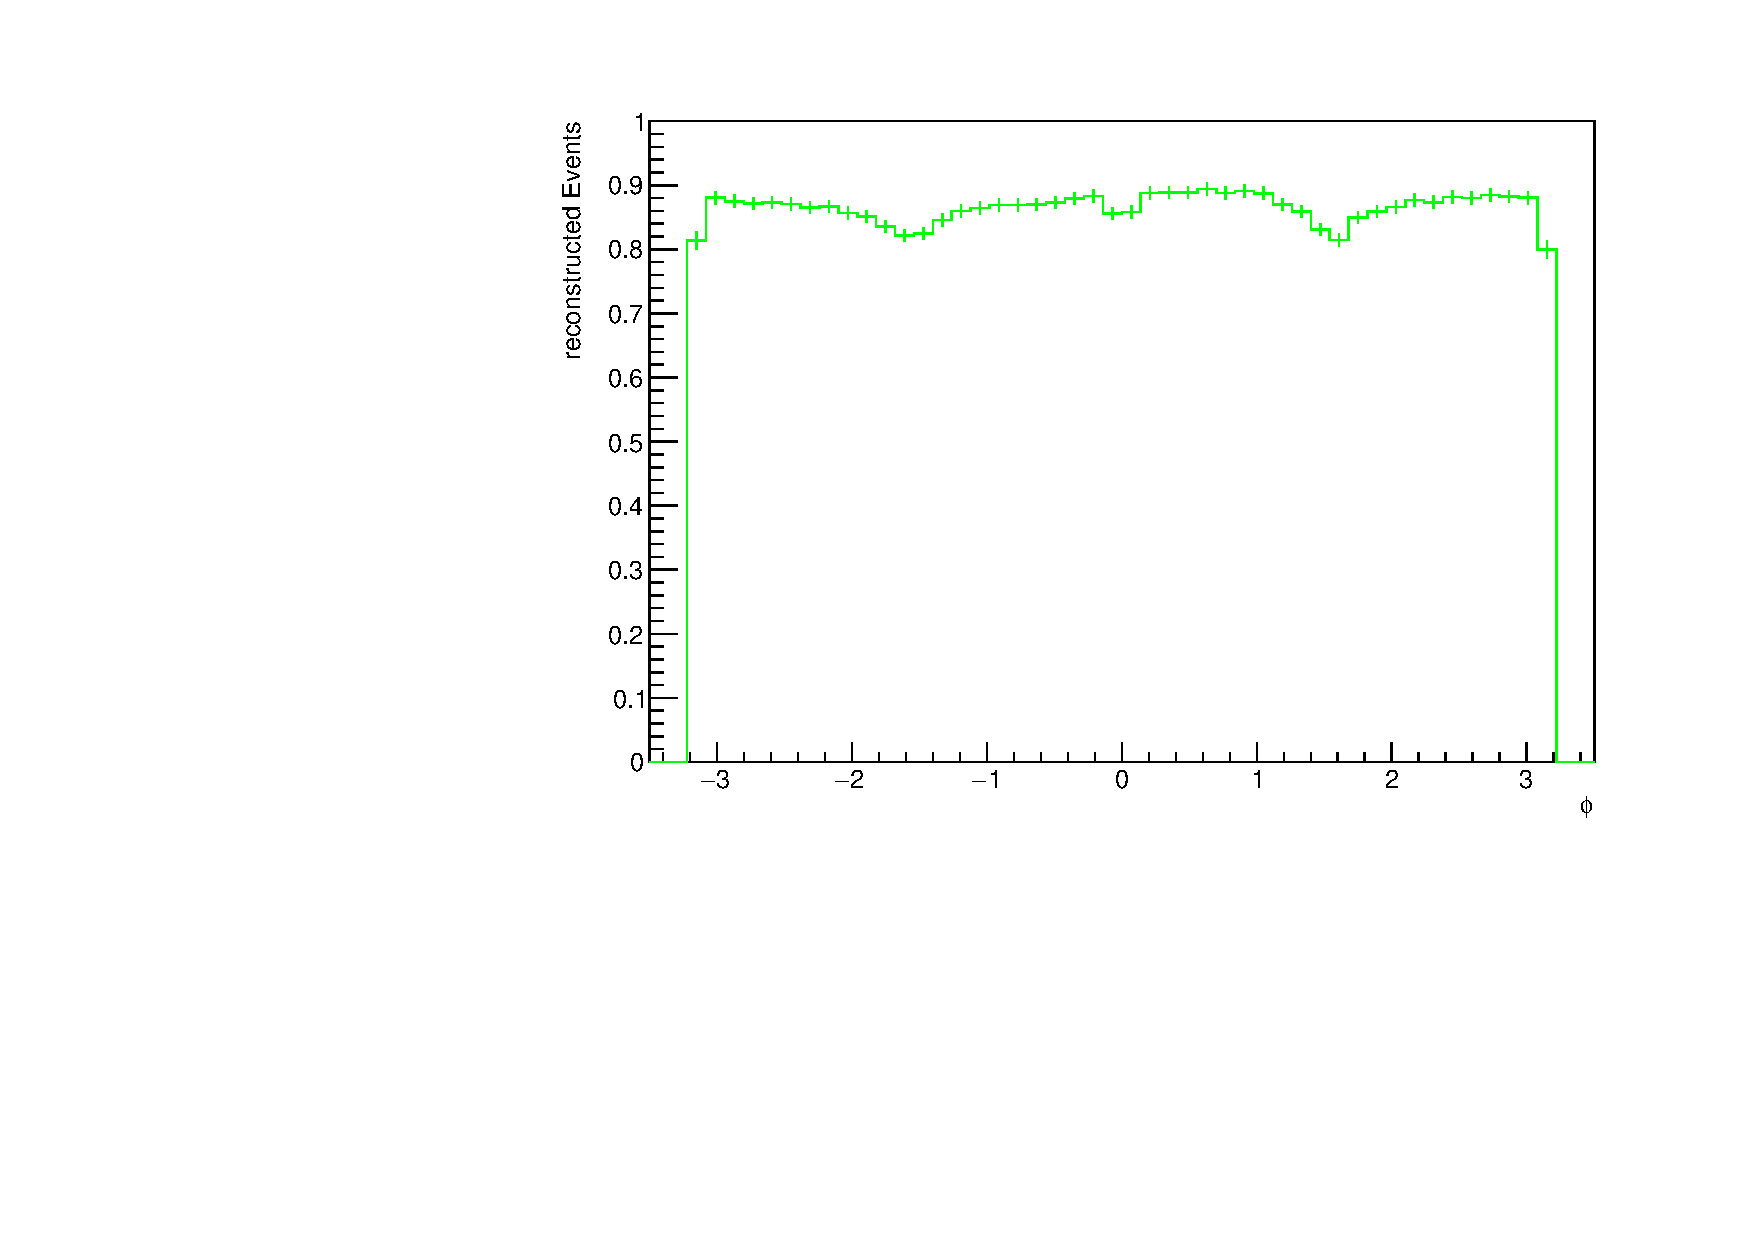
\includegraphics[width=0.9\textwidth]{up_pdf/single/tot/h_phi_reco_Pi.pdf}
\end{subfigure}
\begin{subfigure}{0.45\textwidth}
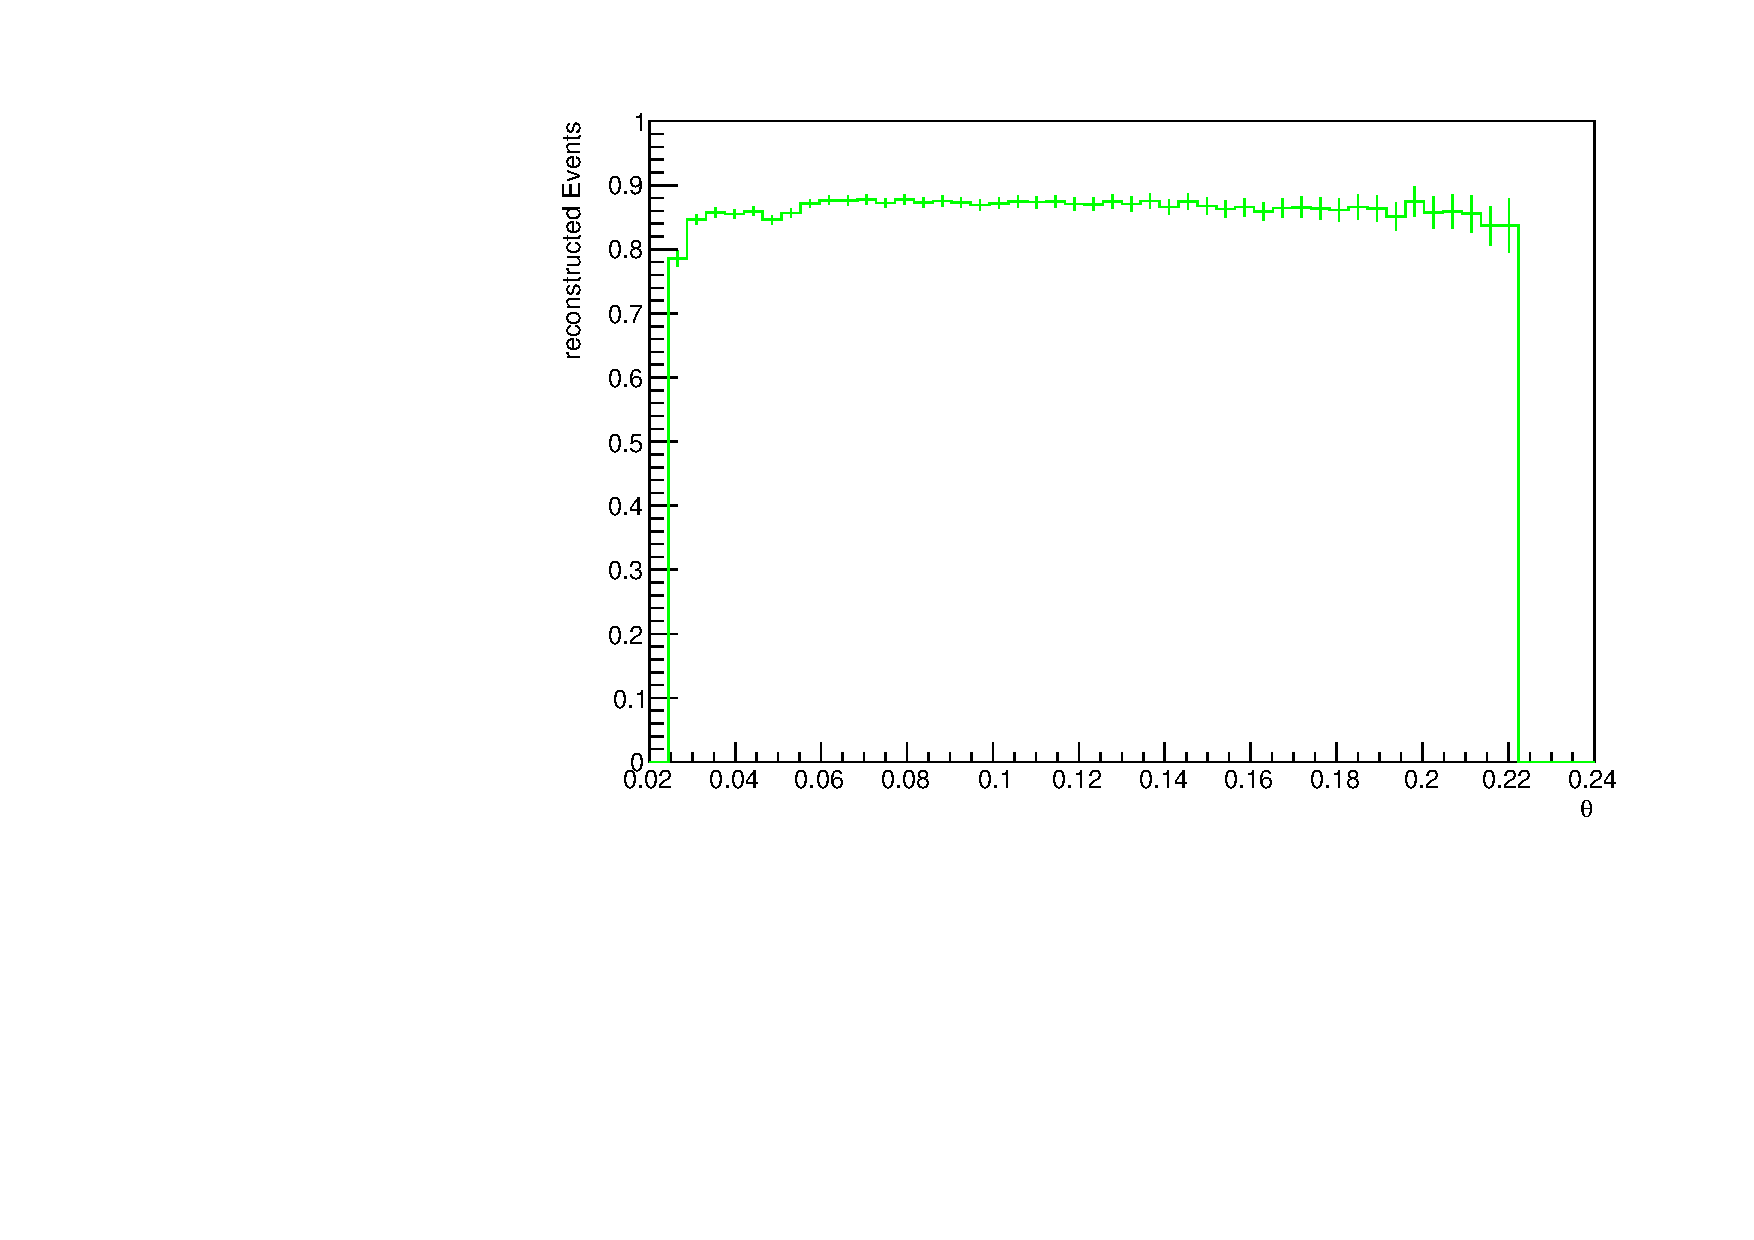
\includegraphics[width=0.9\textwidth]{up_pdf/single/tot/h_theta_reco_Pi.pdf}
\end{subfigure}
\begin{subfigure}{0.45\textwidth}
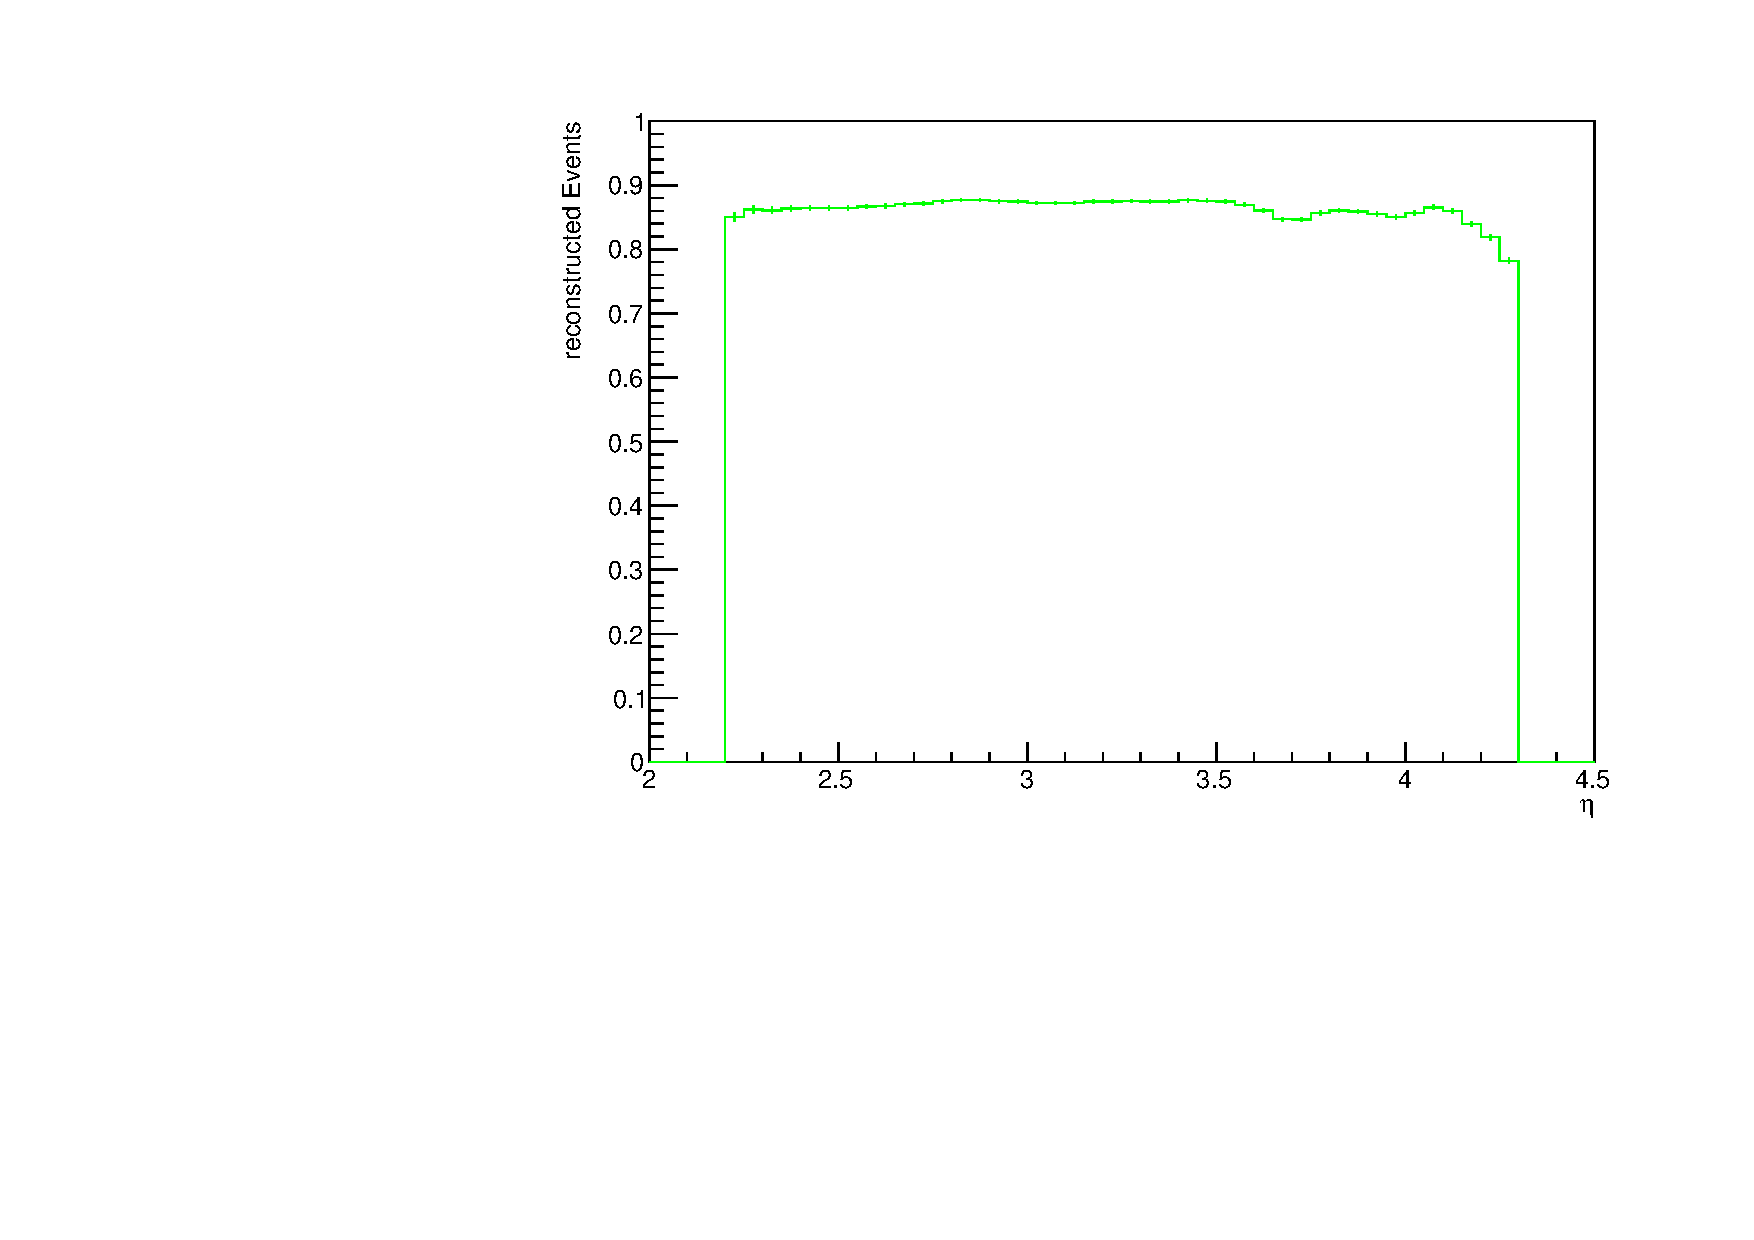
\includegraphics[width=0.9\textwidth]{up_pdf/single/tot/h_eta_reco_Pi.pdf}
\end{subfigure}
\end{figure}
\end{frame}
\begin{frame}{$K$-efficiency}
\begin{figure}
\begin{subfigure}{0.45\textwidth}
\includegraphics[width=0.9\textwidth]{up_pdf/single/tot/h_pt_reco_K.pdf}
\end{subfigure}
\begin{subfigure}{0.45\textwidth}
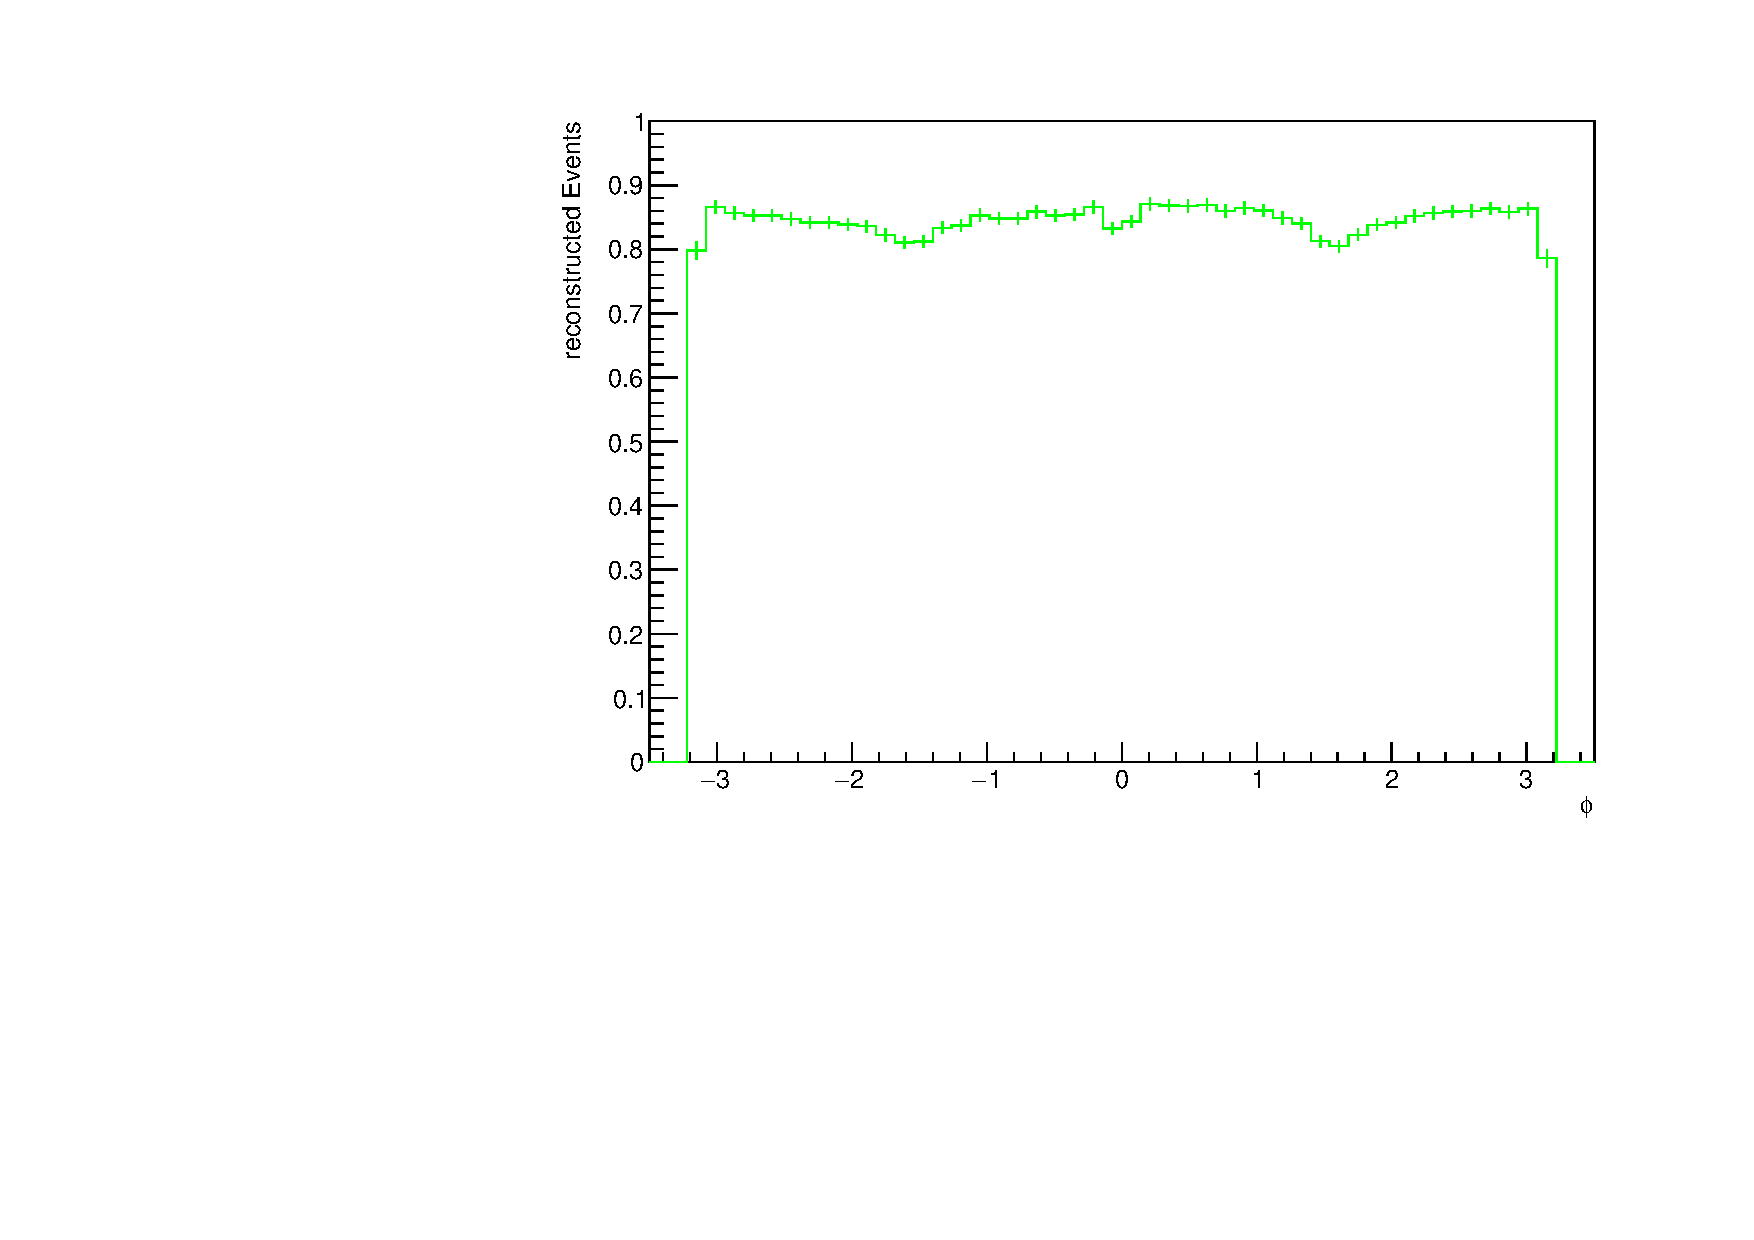
\includegraphics[width=0.9\textwidth]{up_pdf/single/tot/h_phi_reco_K.pdf}
\end{subfigure}
\begin{subfigure}{0.45\textwidth}
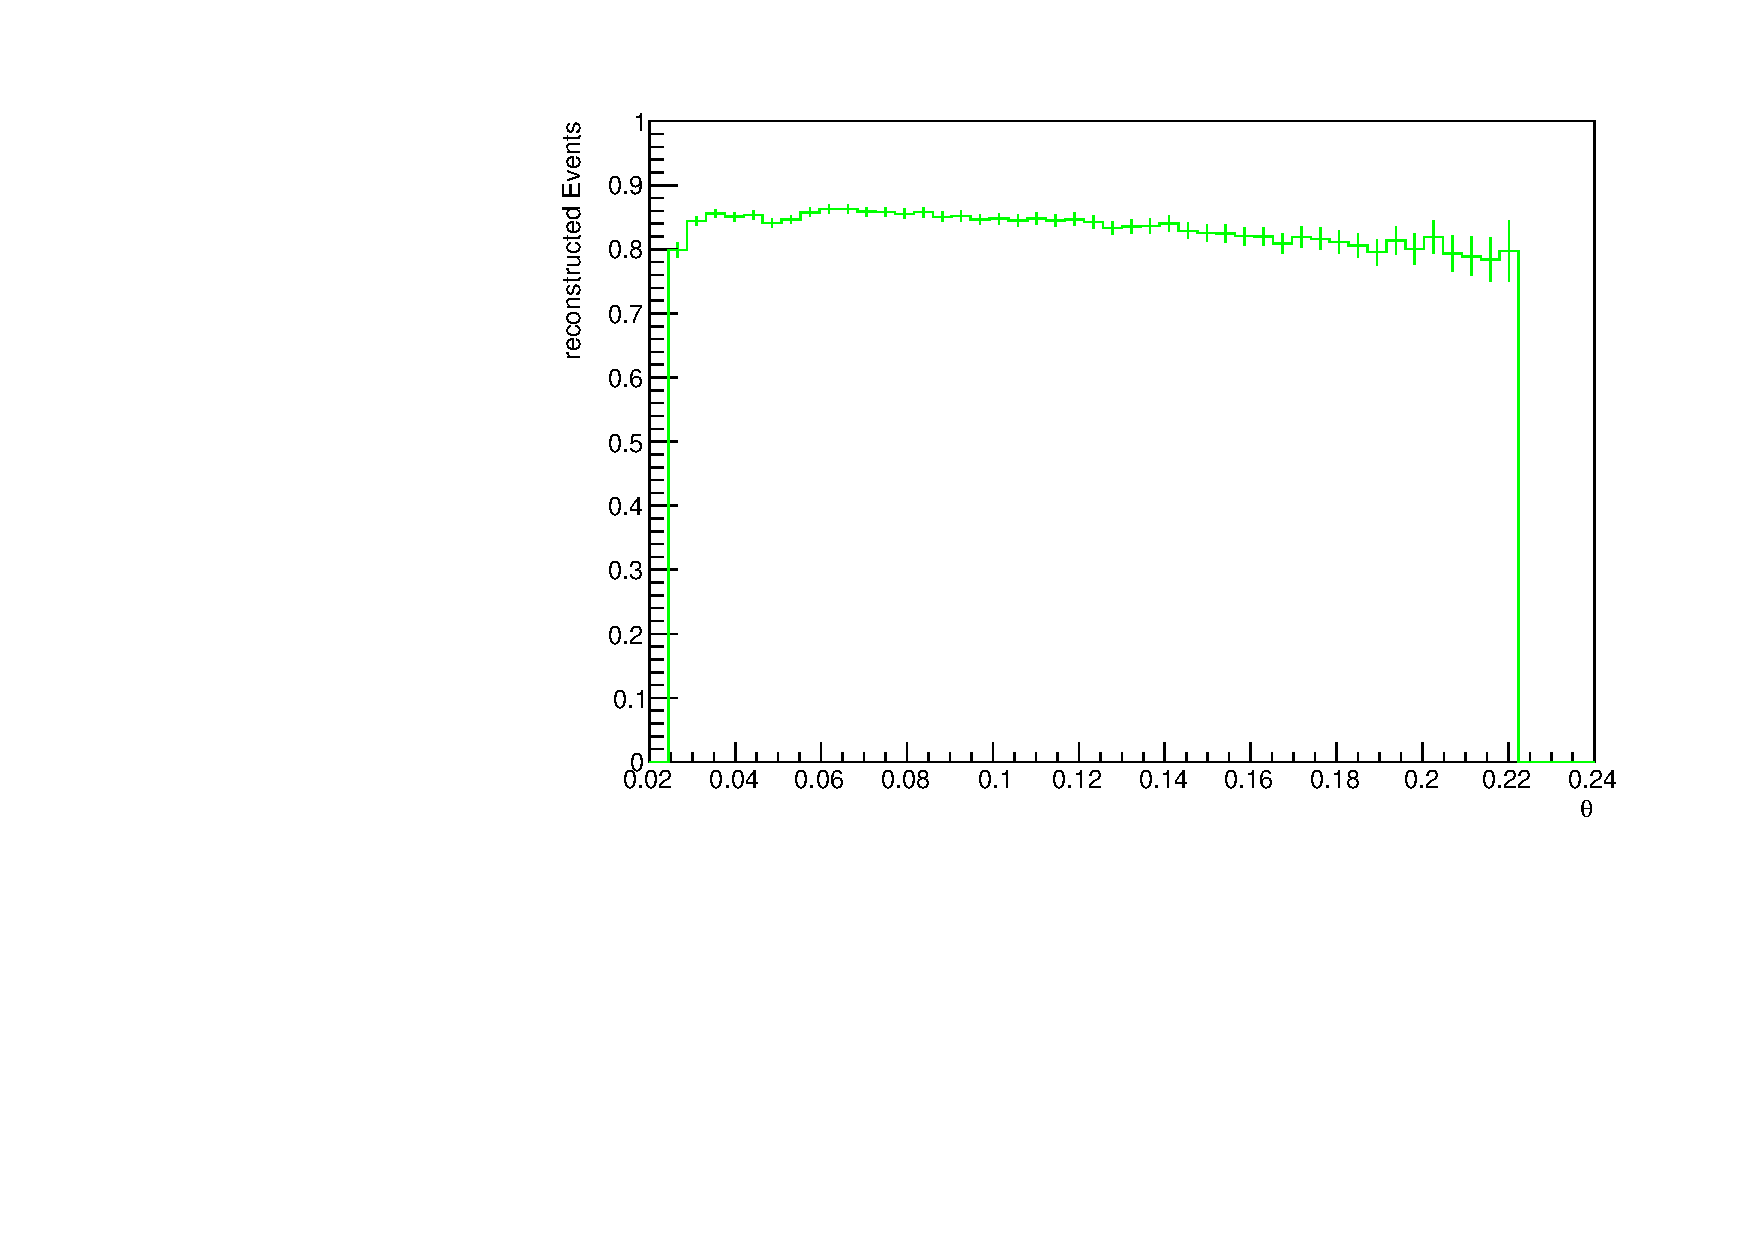
\includegraphics[width=0.9\textwidth]{up_pdf/single/tot/h_theta_reco_K.pdf}
\end{subfigure}
\begin{subfigure}{0.45\textwidth}
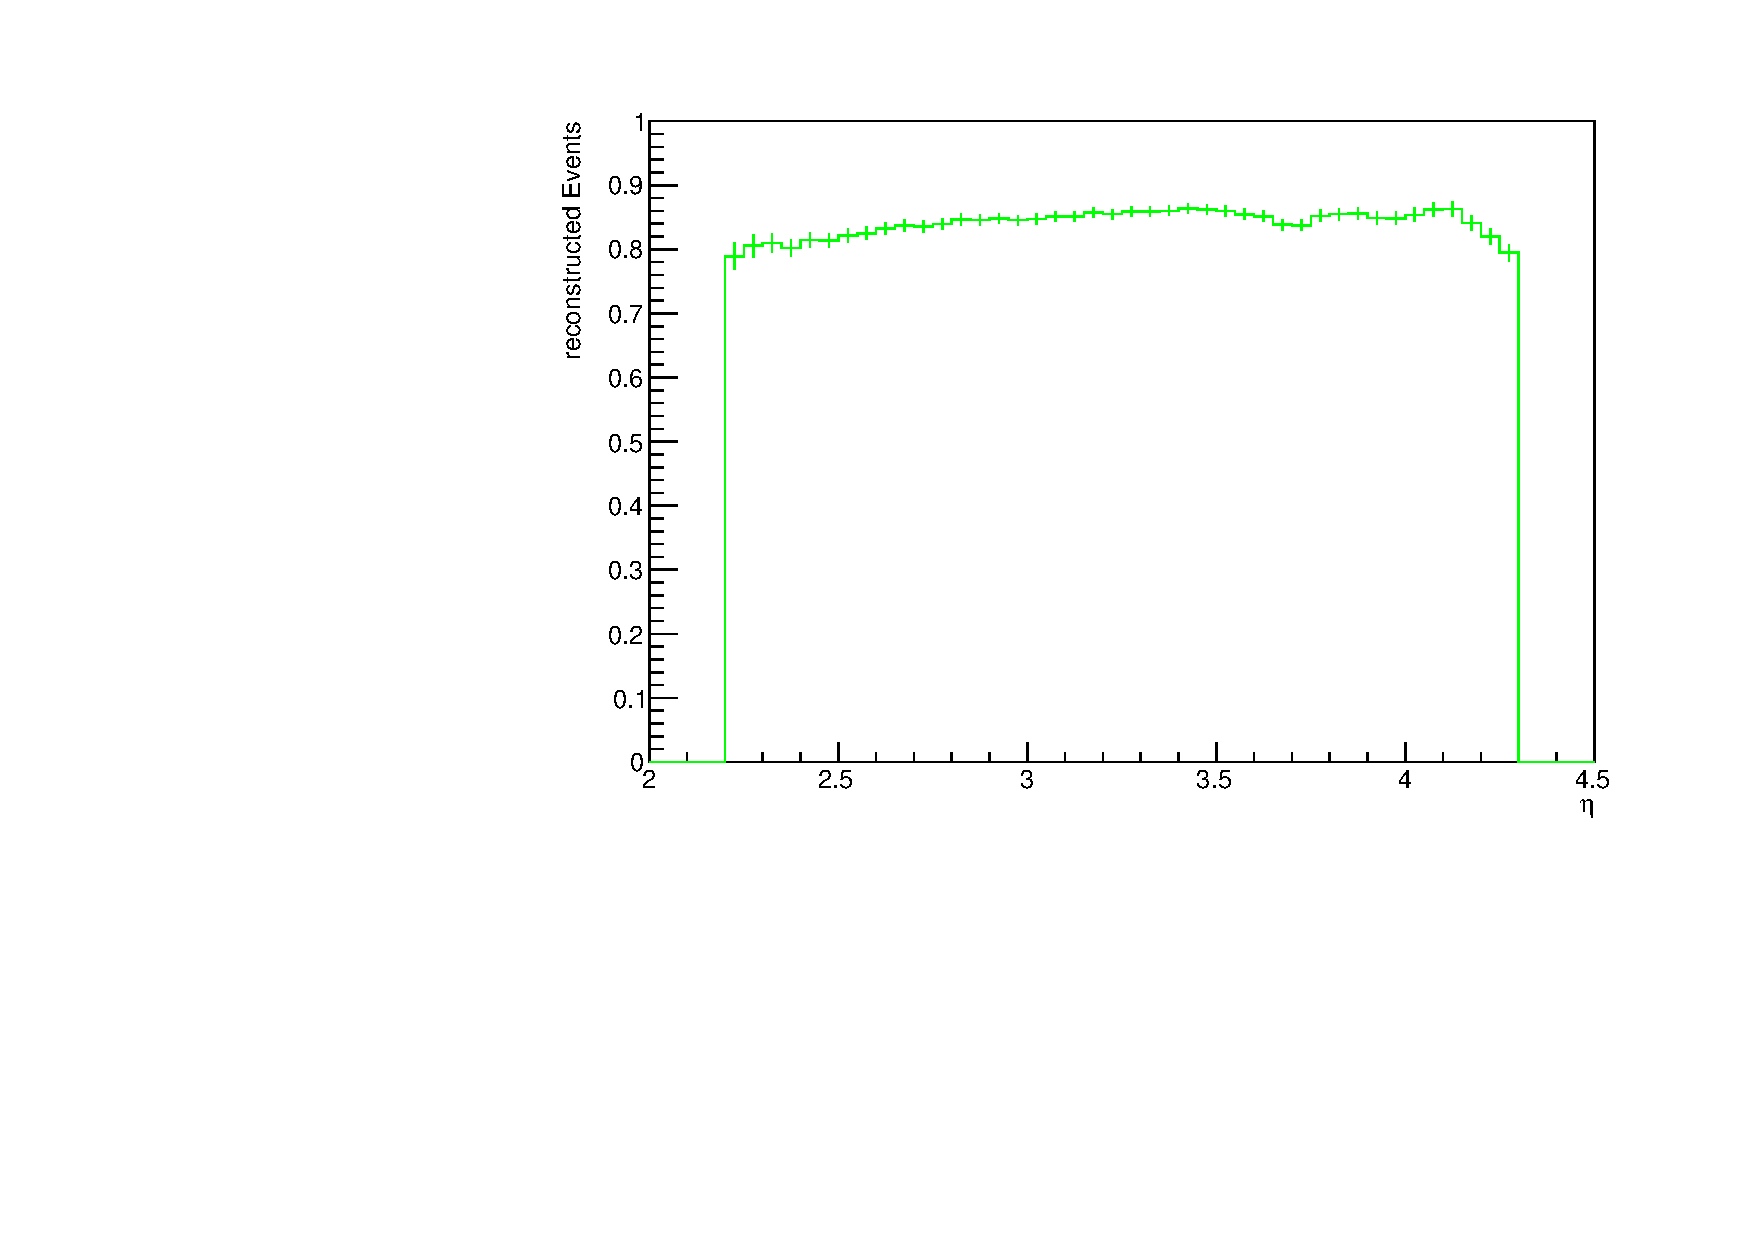
\includegraphics[width=0.9\textwidth]{up_pdf/single/tot/h_eta_reco_K.pdf}
\end{subfigure}
\end{figure}
\end{frame}
\begin{frame}{soft $\pi$-efficiency}
\begin{figure}
\begin{subfigure}{0.45\textwidth}
\includegraphics[width=0.9\textwidth]{up_pdf/single/tot/h_pt_reco_Dst.pdf}
\end{subfigure}
\begin{subfigure}{0.45\textwidth}
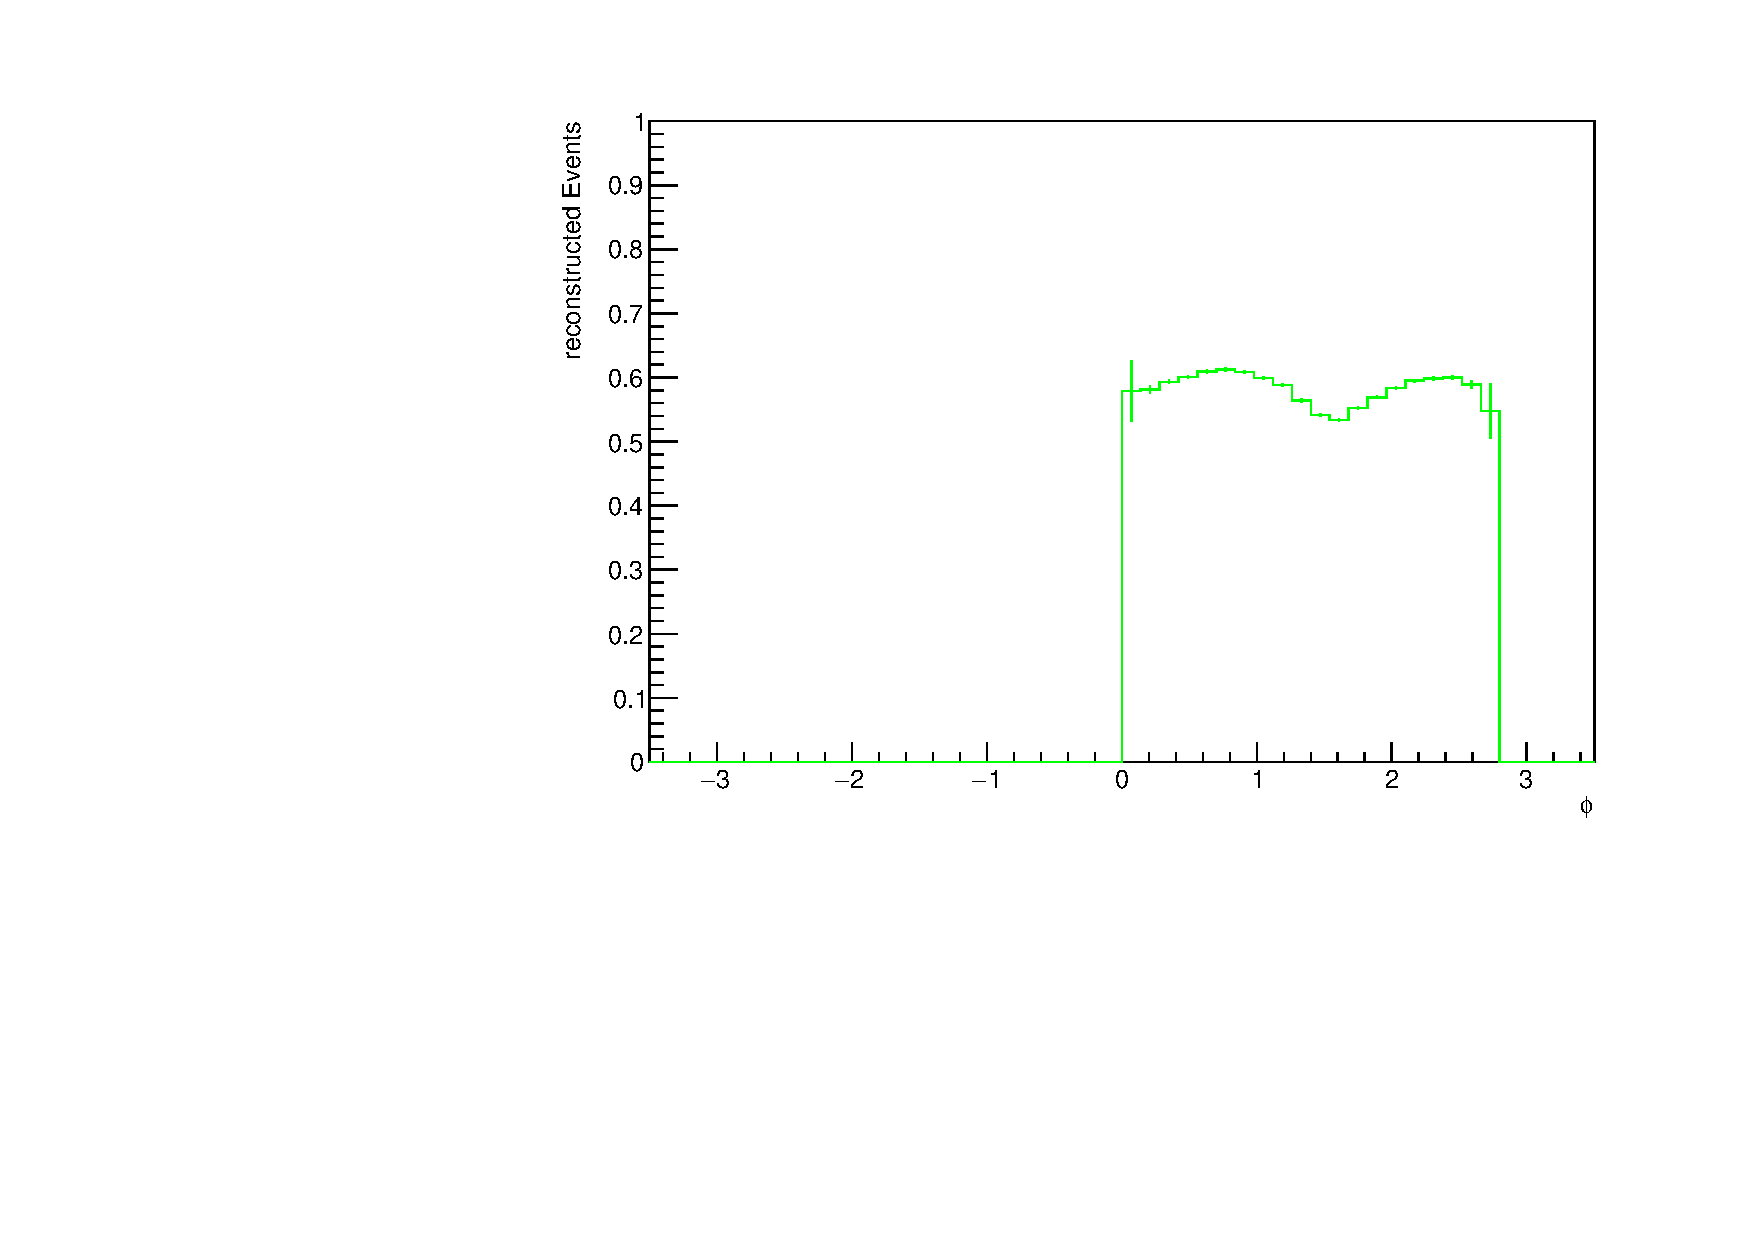
\includegraphics[width=0.9\textwidth]{up_pdf/single/tot/h_phi_reco_Dst.pdf}
\end{subfigure}
\begin{subfigure}{0.45\textwidth}
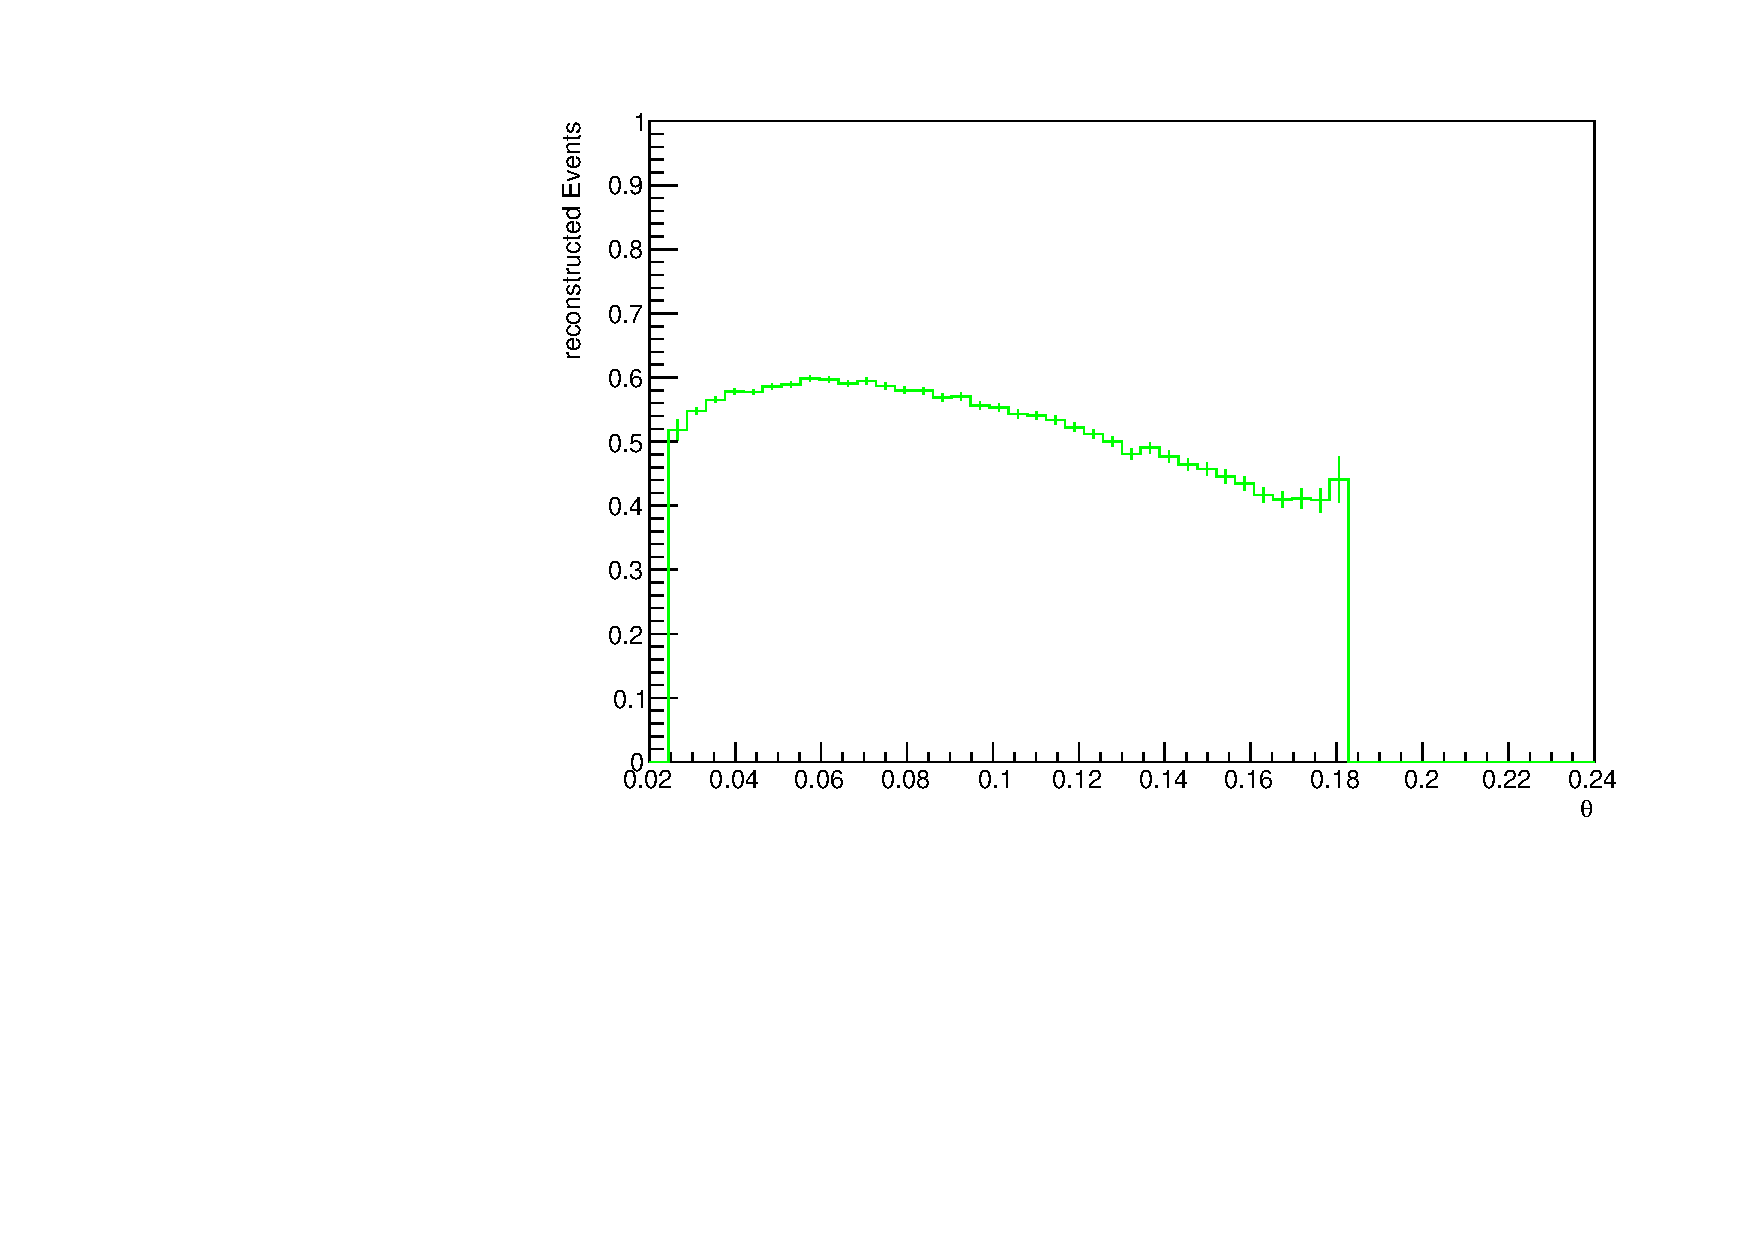
\includegraphics[width=0.9\textwidth]{up_pdf/single/tot/h_theta_reco_Dst.pdf}
\end{subfigure}
\begin{subfigure}{0.45\textwidth}
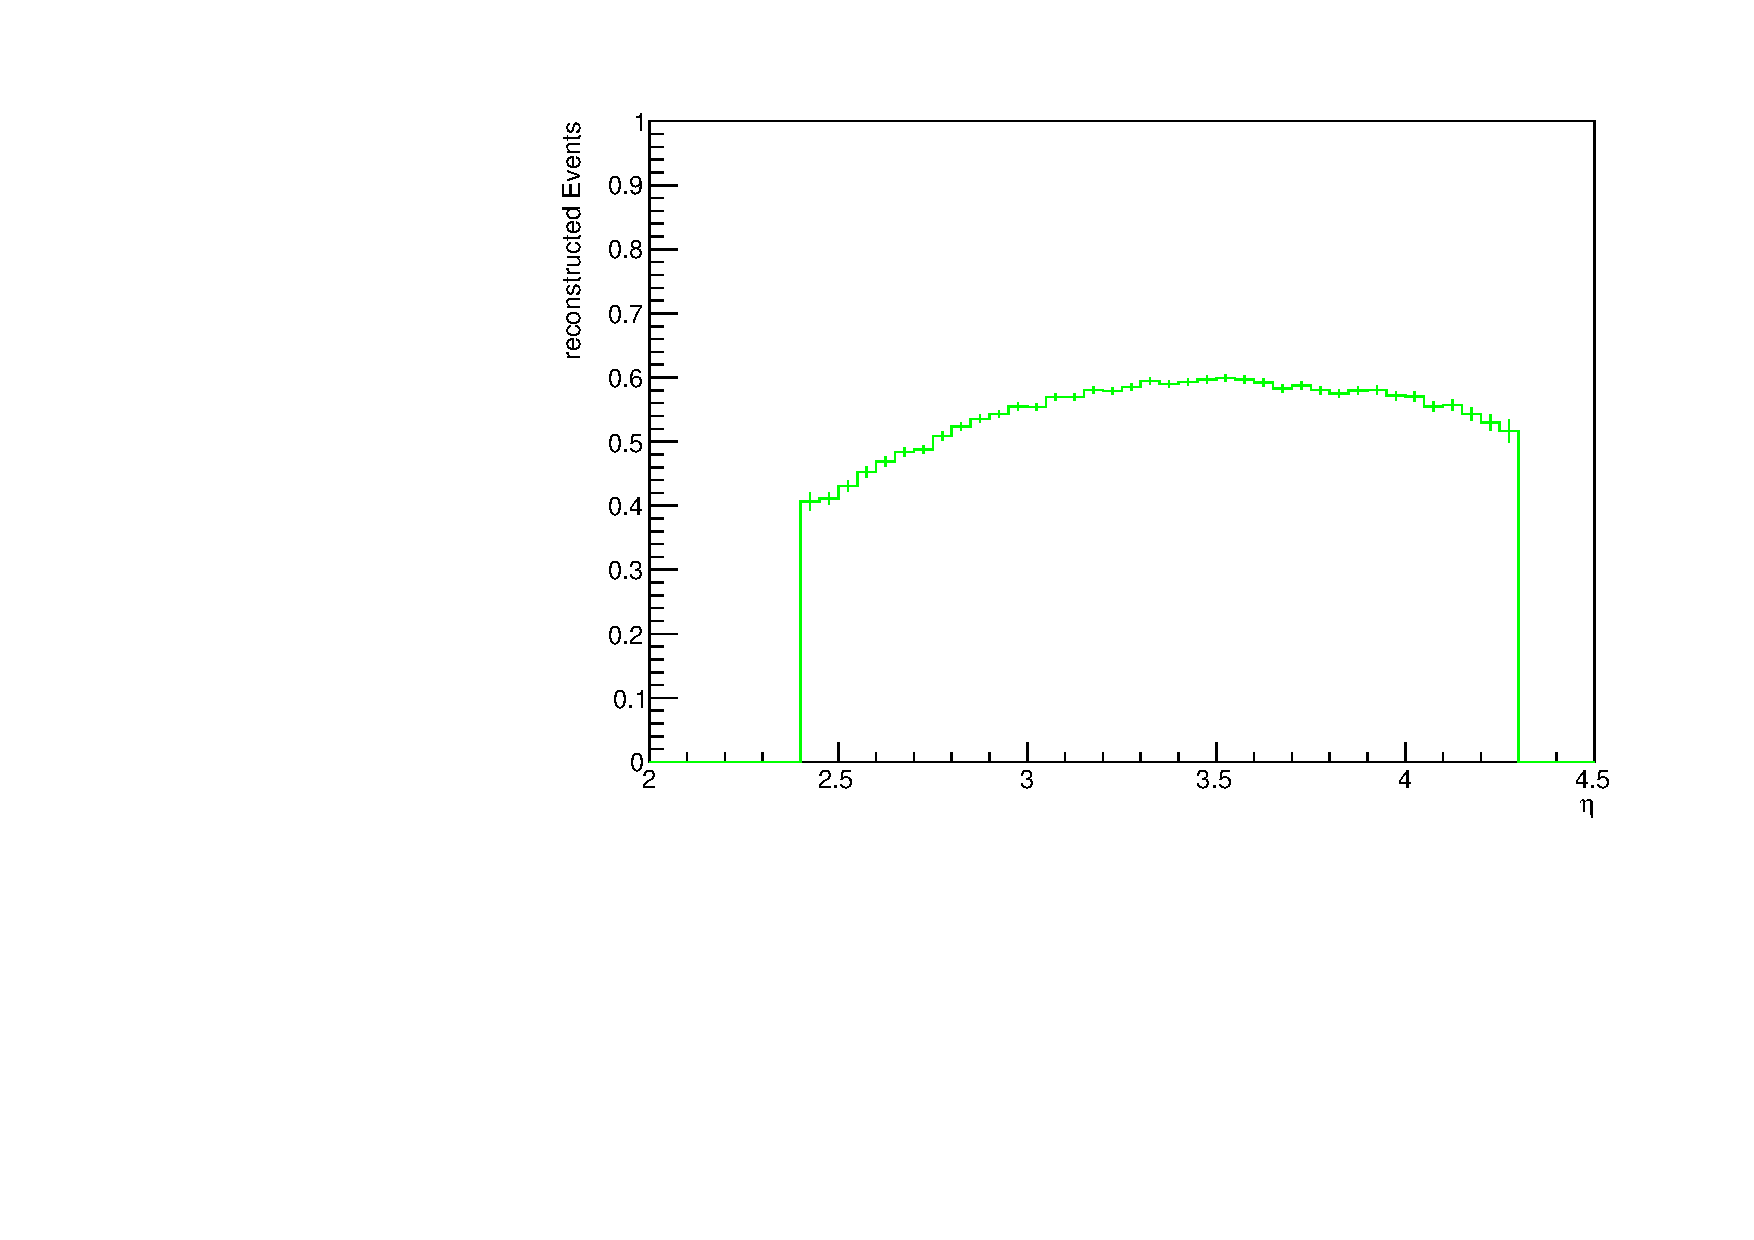
\includegraphics[width=0.9\textwidth]{up_pdf/single/tot/h_eta_reco_Dst.pdf}
\end{subfigure}
\end{figure}
\end{frame}
\begin{frame}{$D^0$-efficiency}
\begin{figure}
\begin{subfigure}{0.45\textwidth}
\includegraphics[width=0.9\textwidth]{up_pdf/single/tot/h_pt_reco_D0.pdf}
\end{subfigure}
\begin{subfigure}{0.45\textwidth}
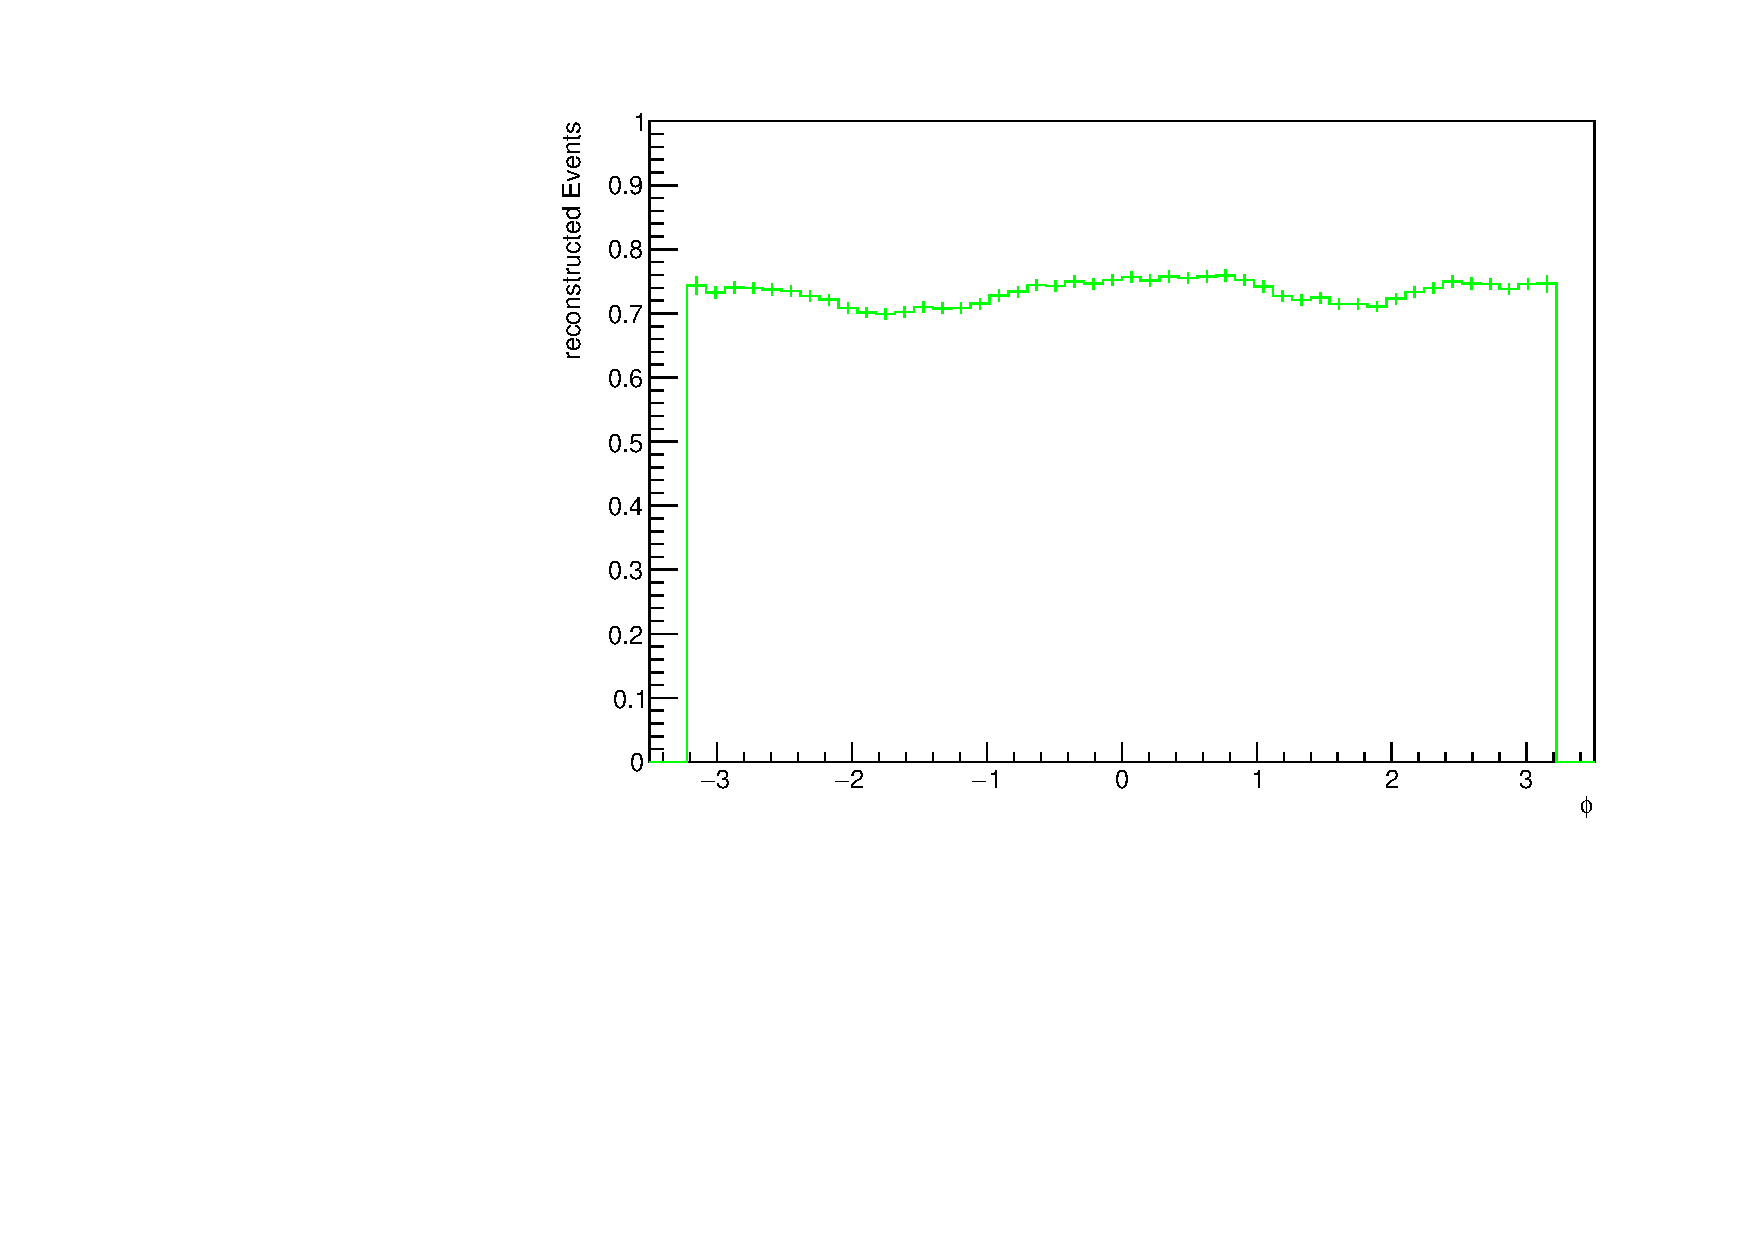
\includegraphics[width=0.9\textwidth]{up_pdf/single/tot/h_phi_reco_D0.pdf}
\end{subfigure}
\begin{subfigure}{0.45\textwidth}
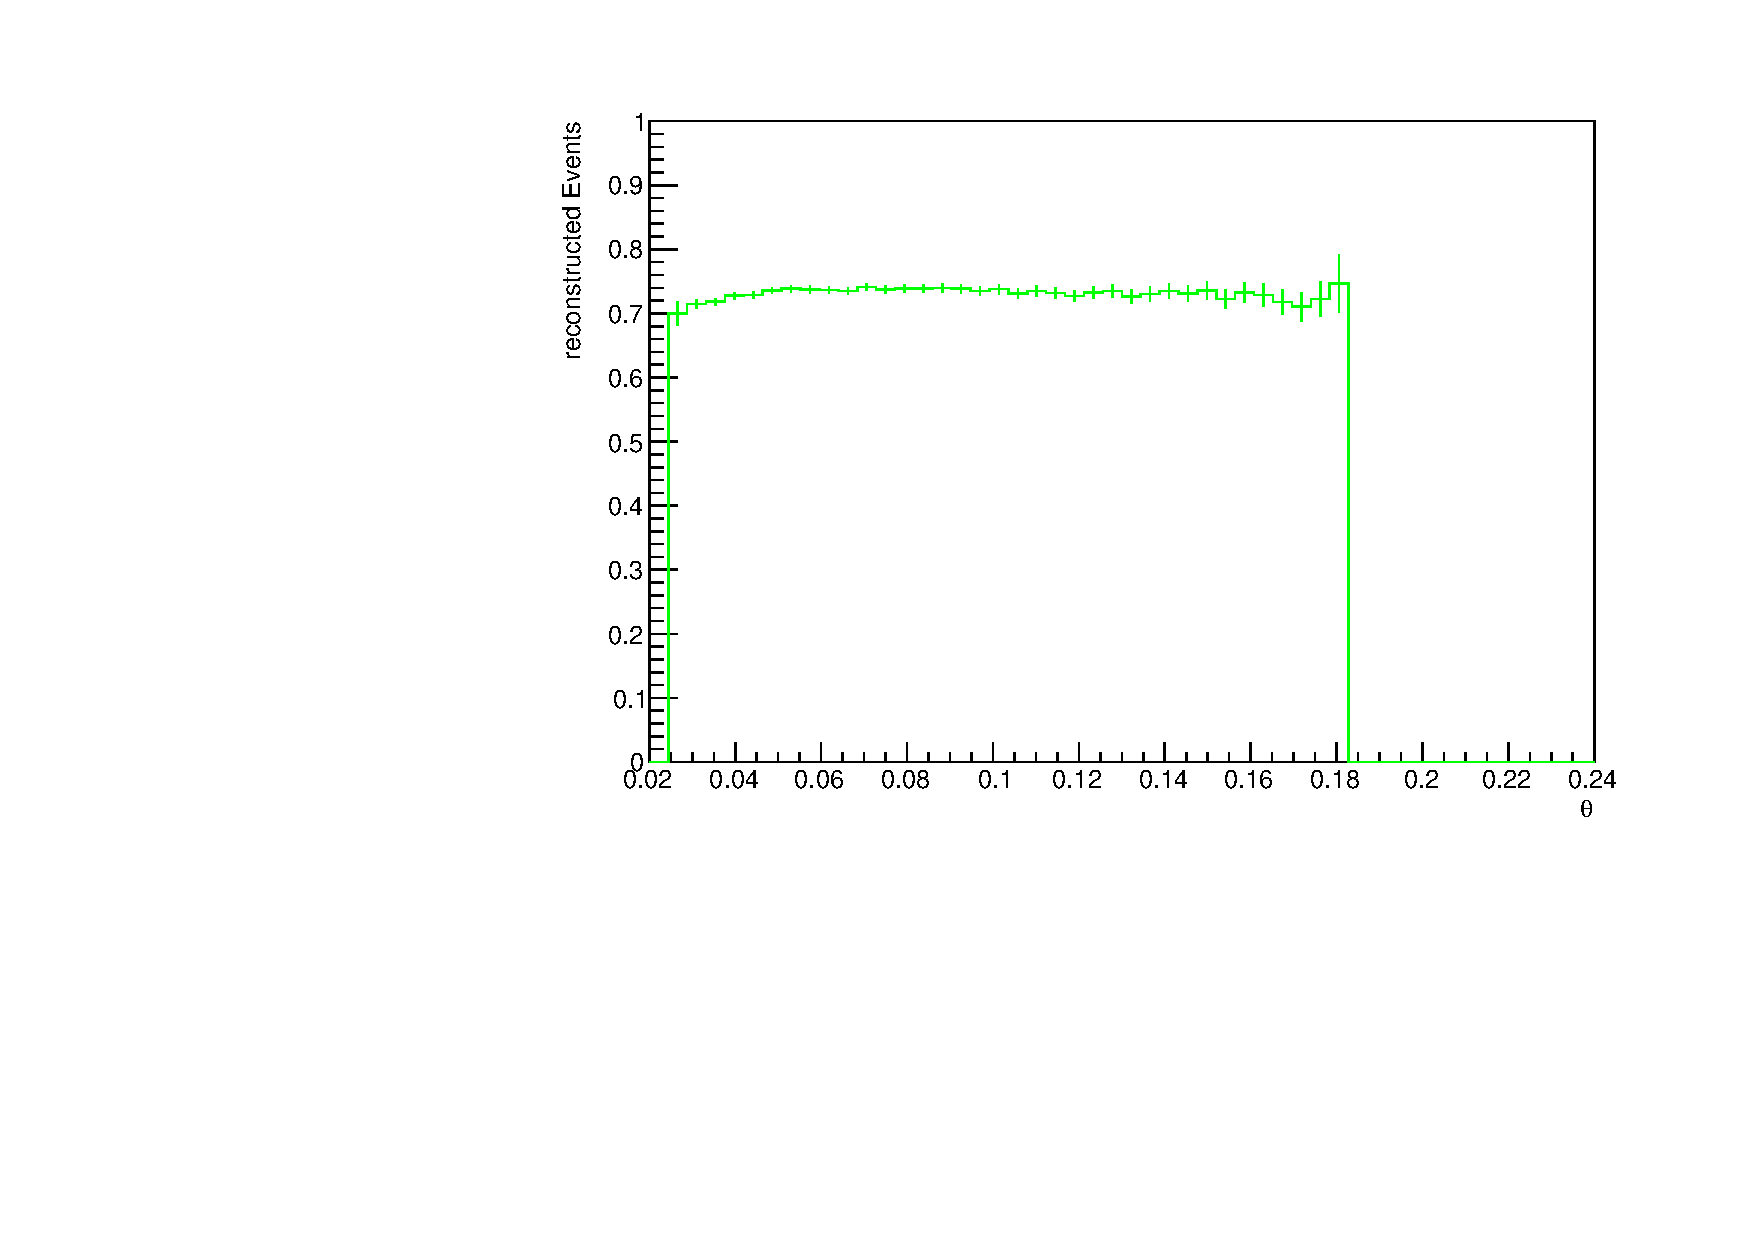
\includegraphics[width=0.9\textwidth]{up_pdf/single/tot/h_theta_reco_D0.pdf}
\end{subfigure}
\begin{subfigure}{0.45\textwidth}
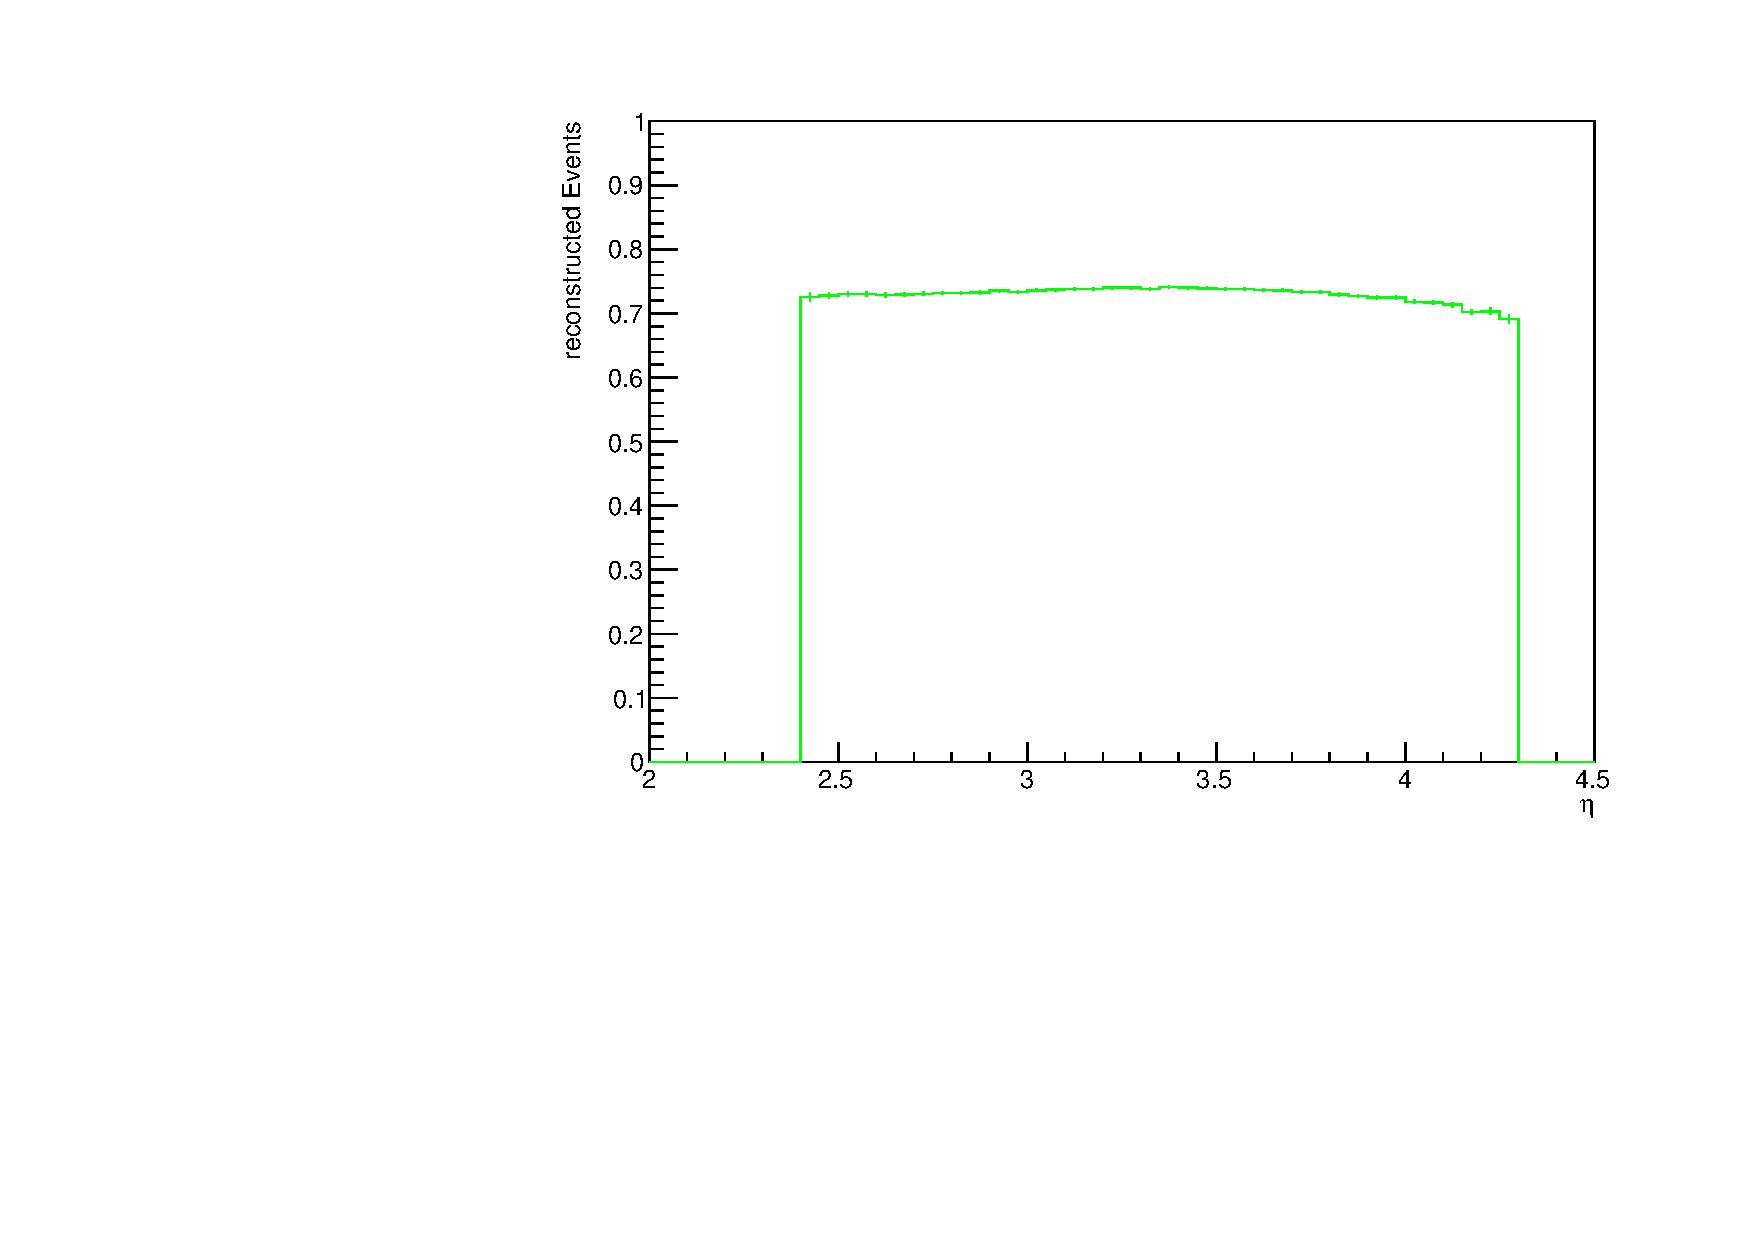
\includegraphics[width=0.9\textwidth]{up_pdf/single/tot/h_eta_reco_D0.pdf}
\end{subfigure}
\end{figure}
\end{frame}
\begin{frame}{$D^*$-efficiency}
\begin{figure}
\begin{subfigure}{0.45\textwidth}
\includegraphics[width=0.9\textwidth]{up_pdf/single/tot/h_pt_reco_Dst.pdf}
\end{subfigure}
\begin{subfigure}{0.45\textwidth}
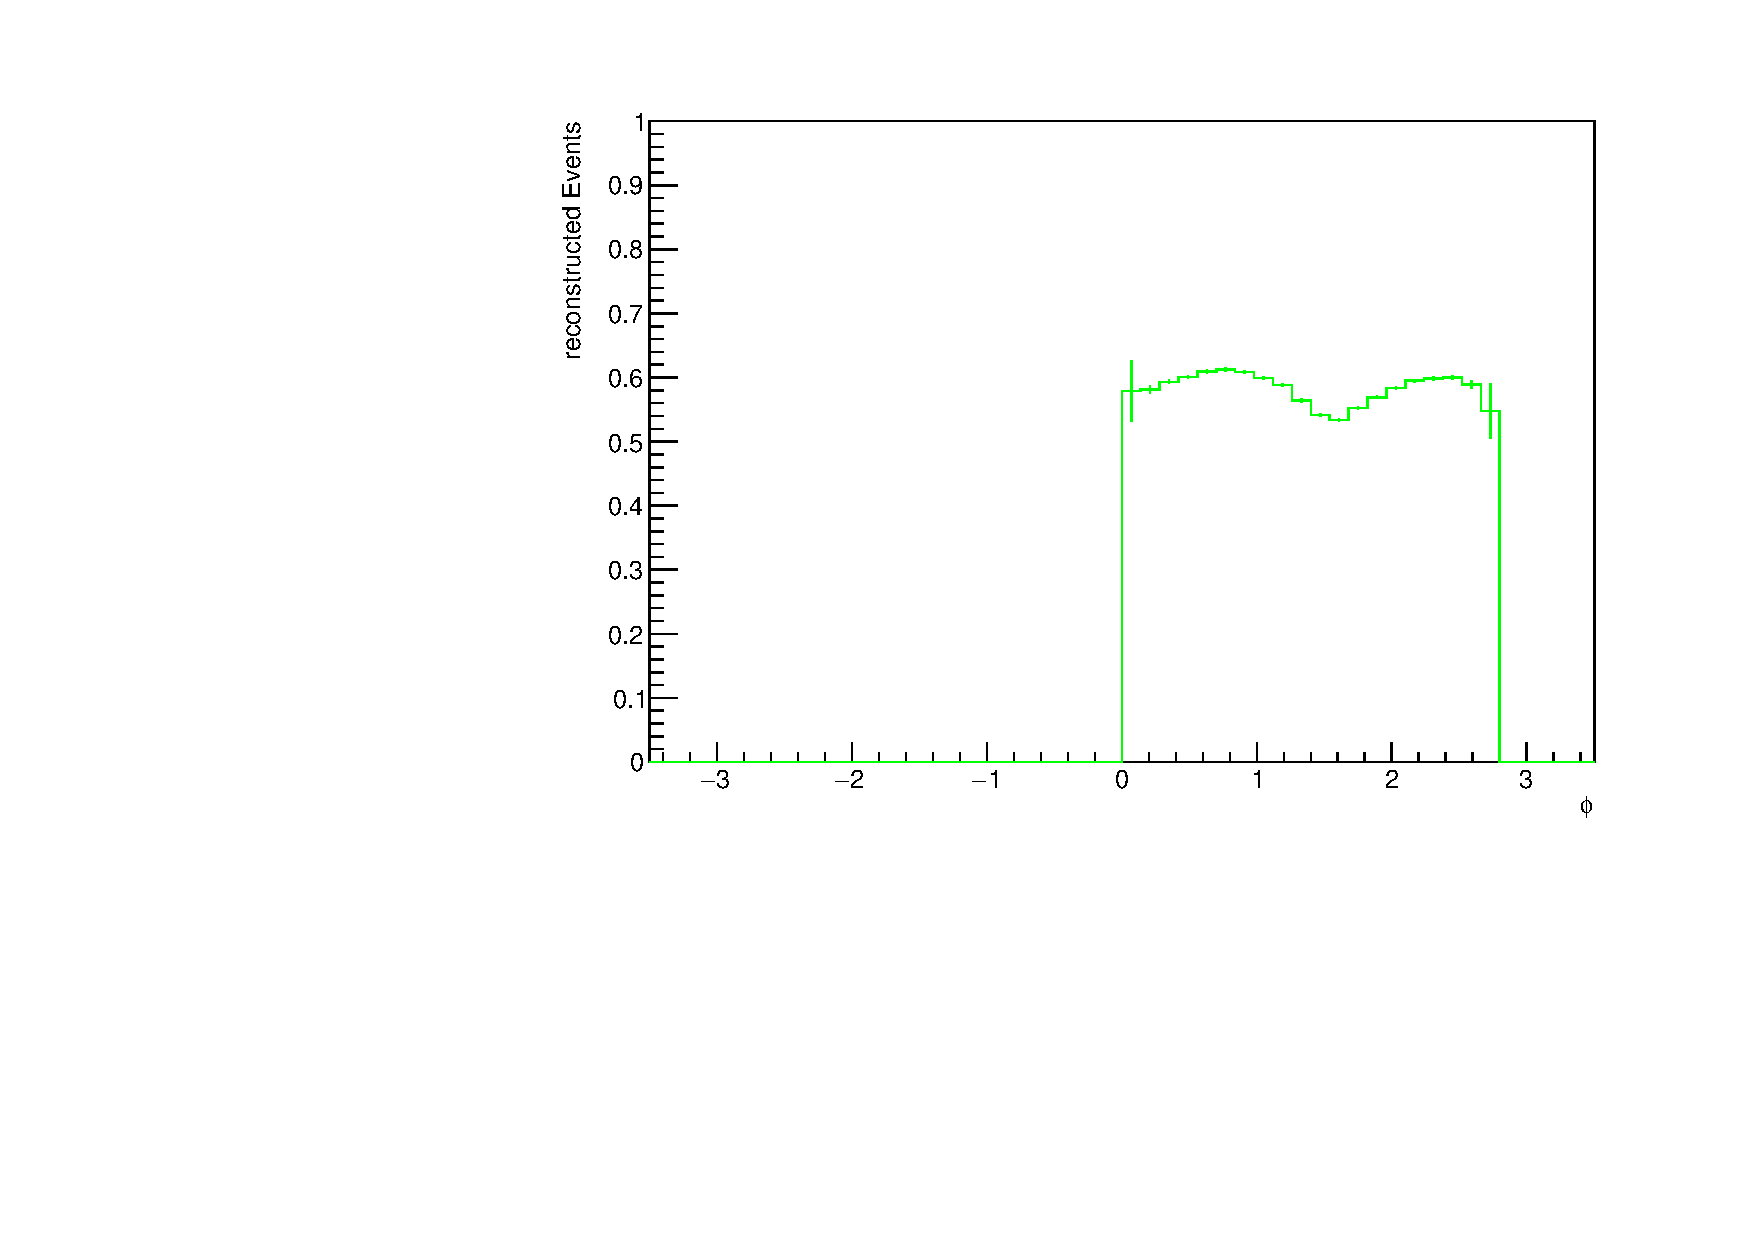
\includegraphics[width=0.9\textwidth]{up_pdf/single/tot/h_phi_reco_Dst.pdf}
\end{subfigure}
\begin{subfigure}{0.45\textwidth}
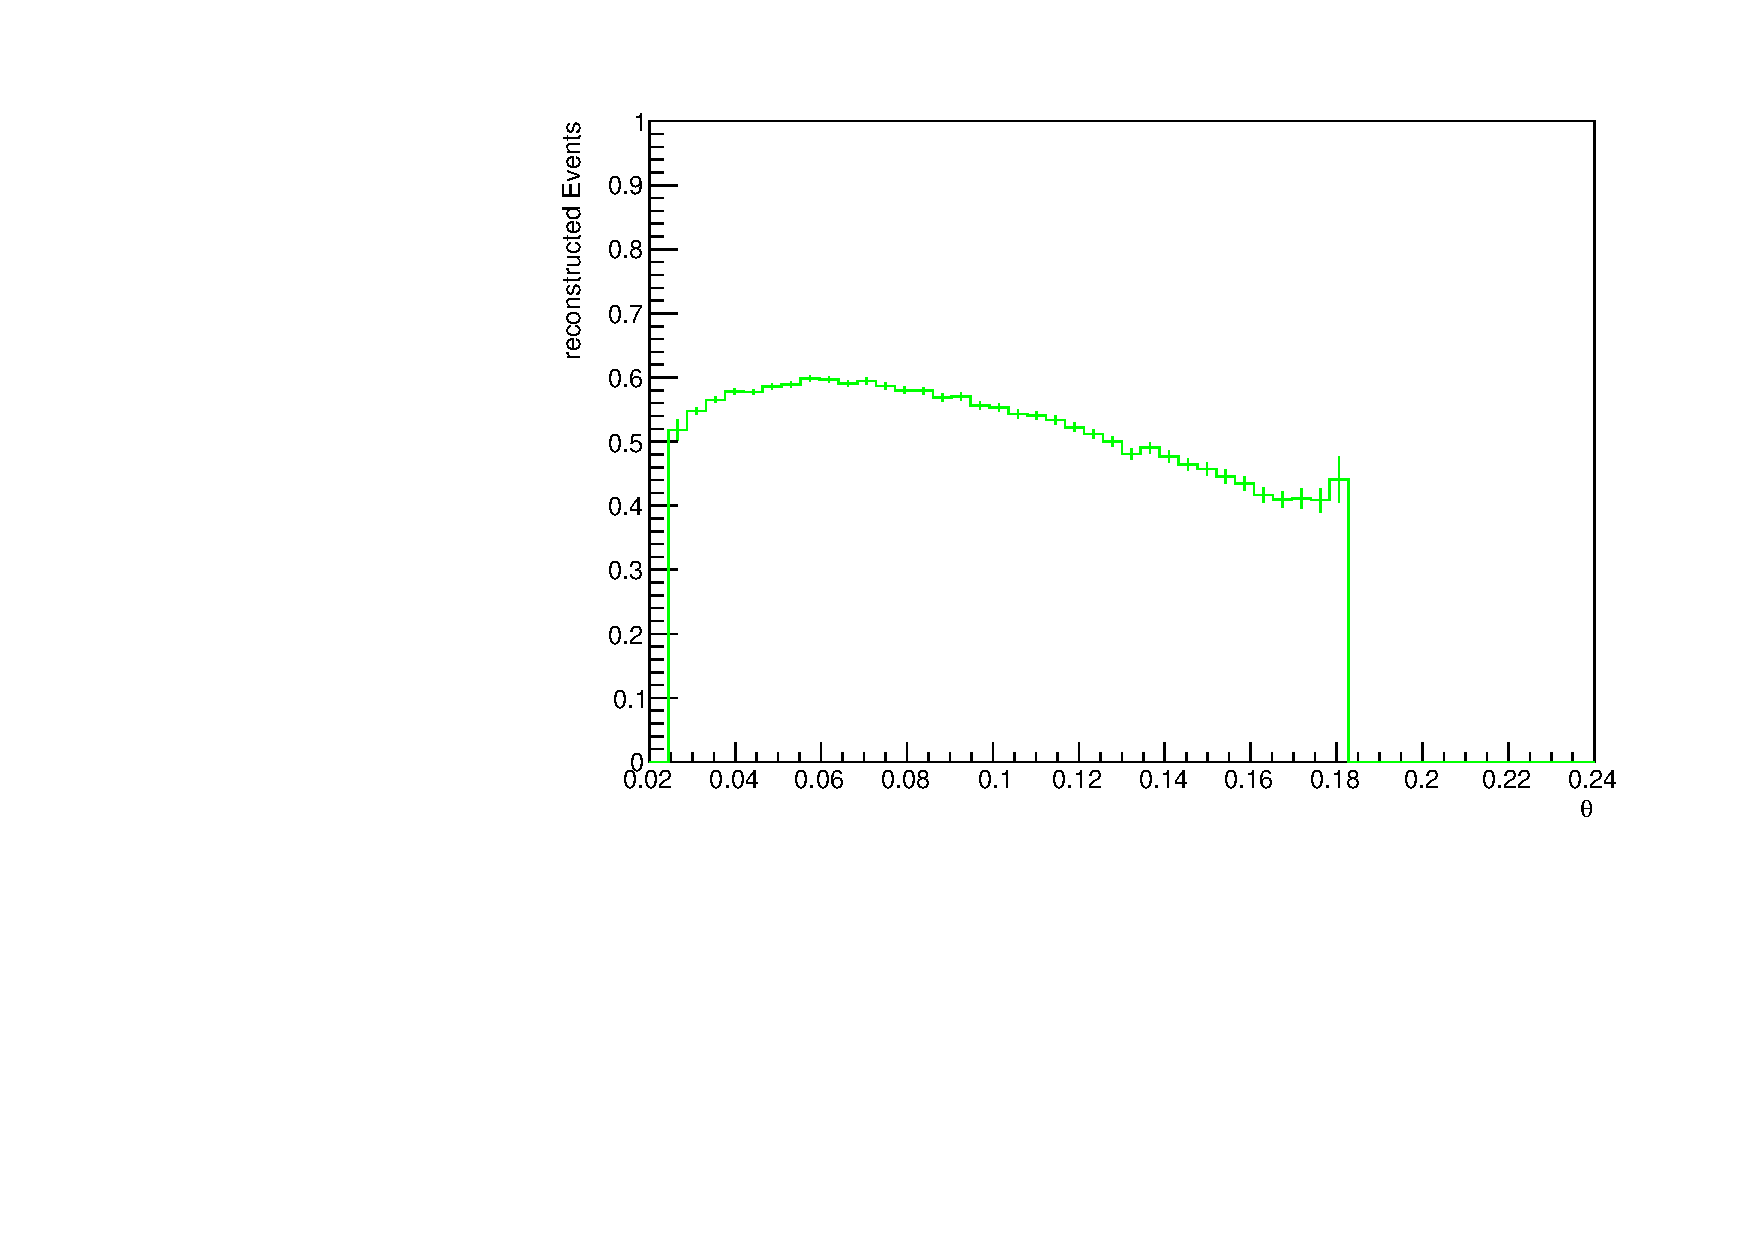
\includegraphics[width=0.9\textwidth]{up_pdf/single/tot/h_theta_reco_Dst.pdf}
\end{subfigure}
\begin{subfigure}{0.45\textwidth}
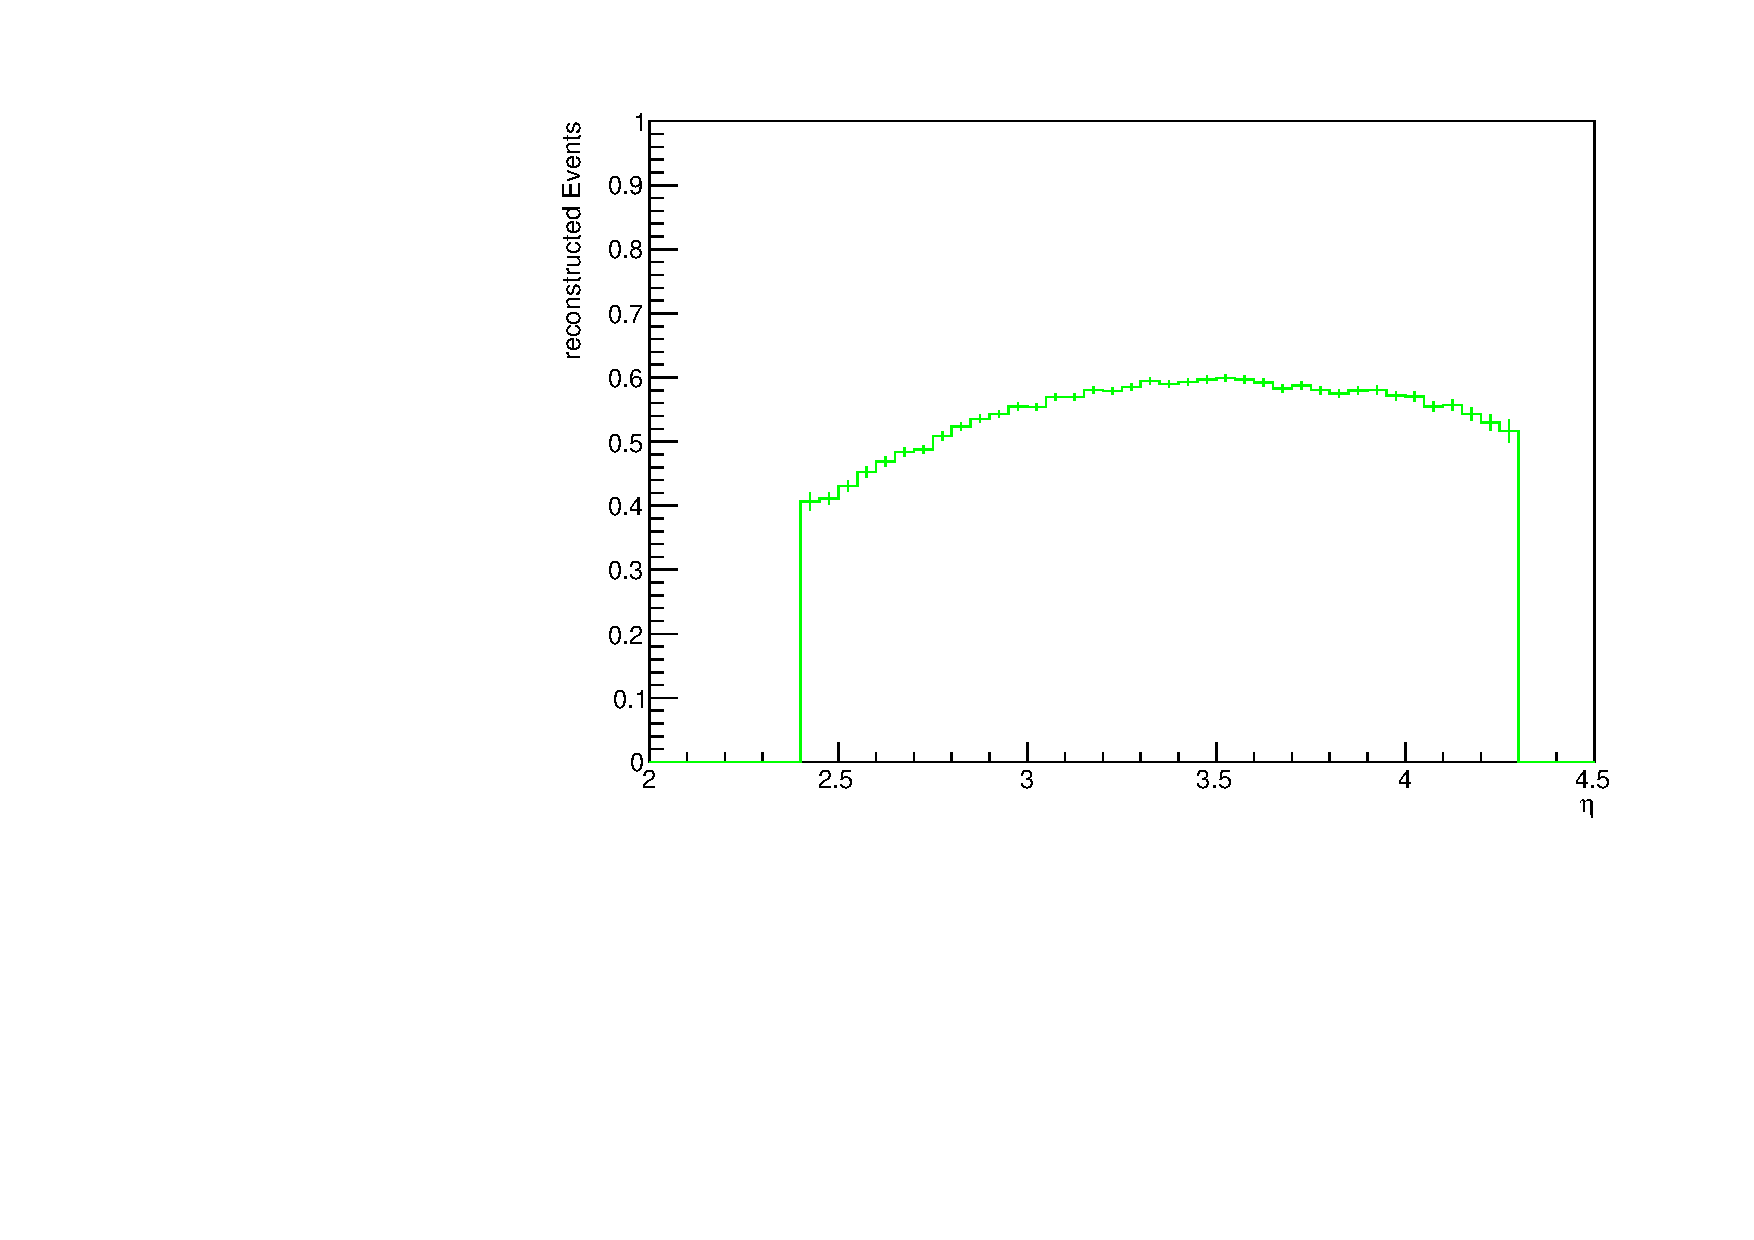
\includegraphics[width=0.9\textwidth]{up_pdf/single/tot/h_eta_reco_Dst.pdf}
\end{subfigure}
\end{figure}
\end{frame}
\begin{frame}
\begin{LARGE}
\textbf{Charge: +}
\end{LARGE}
\end{frame}
\begin{frame}{Efficiencies}
\begin{table}
\resizebox{\textwidth}{!}{
%	\caption{Reconstruction efficiencies for different polarities}
	\begin{tabular}{cS[table-format=2.2]@{${}\pm{}$}S[table-format=1.2]S[table-format=2.2]@{${}\pm{}$}S[table-format=1.2]S[table-format=2.2]@{${}\pm{}$}S[table-format=1.2]S[table-format=2.2]@{${}\pm{}$}S[table-format=1.2]S[table-format=2.2]@{${}\pm{}$}S[table-format=1.2]}
		\toprule
		{Polarity} & \multicolumn{2}{c}{$\epsilon_{\pi} $} & \multicolumn{2}{c}{$\epsilon_{K} $} & \multicolumn{2}{c}{$ \epsilon_{\pi,s} $} & \multicolumn{2}{c}{$\epsilon_{D^0} $} & \multicolumn{2}{c}{$\epsilon_{D^*} $} \\
		\midrule
		$UP$ & 86.66 & 0.02 & 85.02 & 0.02 & 76.37 & 0.02 & 73.01 & 0.03 & 55.86 & 0.03 \\
		$DOWN$ & 86.70 & 0.02 & 85.07 & 0.02 & 76.98 & 0.02 & 73.06 & 0.03 & 56.33 & 0.03 \\
		\bottomrule
	\end{tabular}}
\resizebox{\textwidth}{!}{
%	\caption{UP Polarity - reconstructed vs. total number of events}
	\begin{tabular}{cS[table-format=6.0]S[table-format=6.0]S[table-format=6.0]S[table-format=6.0]S[table-format=6.0]}
		\toprule
		{UP} & {$\pi $} & {$K $} & {$ soft\, \pi $} & {$D^0 $} & {$D^* $} \\
		\midrule
		$N_\text{reco}$ & 2669990 & 2620280 & 2352910 & 2249370 & 1720940 \\
		$N_\text{tot}$ & 3081050 & 3082060 & 3081050 & 3081050 & 3081050 \\
		\bottomrule
	\end{tabular}}
\resizebox{\textwidth}{!}{
%	\caption{DOWN Polarity - reconstructed vs. total number of events}
	\begin{tabular}{cS[table-format=6.0]S[table-format=6.0]S[table-format=6.0]S[table-format=6.0]S[table-format=6.0]}
		\toprule
		{DOWN} & {$\pi $} & {$K $} & {$ soft\, \pi $} & {$D^0 $} & {$D^* $} \\
		\midrule
		$N_\text{reco}$ & 2674000 & 2626350 & 2374360 & 2253370 & 1737460 \\
		$N_\text{tot}$ & 3084220 & 3087370 & 3084220 & 3084220 & 3084220 \\
		\bottomrule
	\end{tabular}}
\end{table}
\end{frame}
\begin{frame}{$\pi$-efficiency}
\begin{figure}
\begin{subfigure}{0.45\textwidth}
\includegraphics[width=0.9\textwidth]{up_pdf/single/pos/h_pt_reco_Pi_pos.pdf}
\end{subfigure}
\begin{subfigure}{0.45\textwidth}
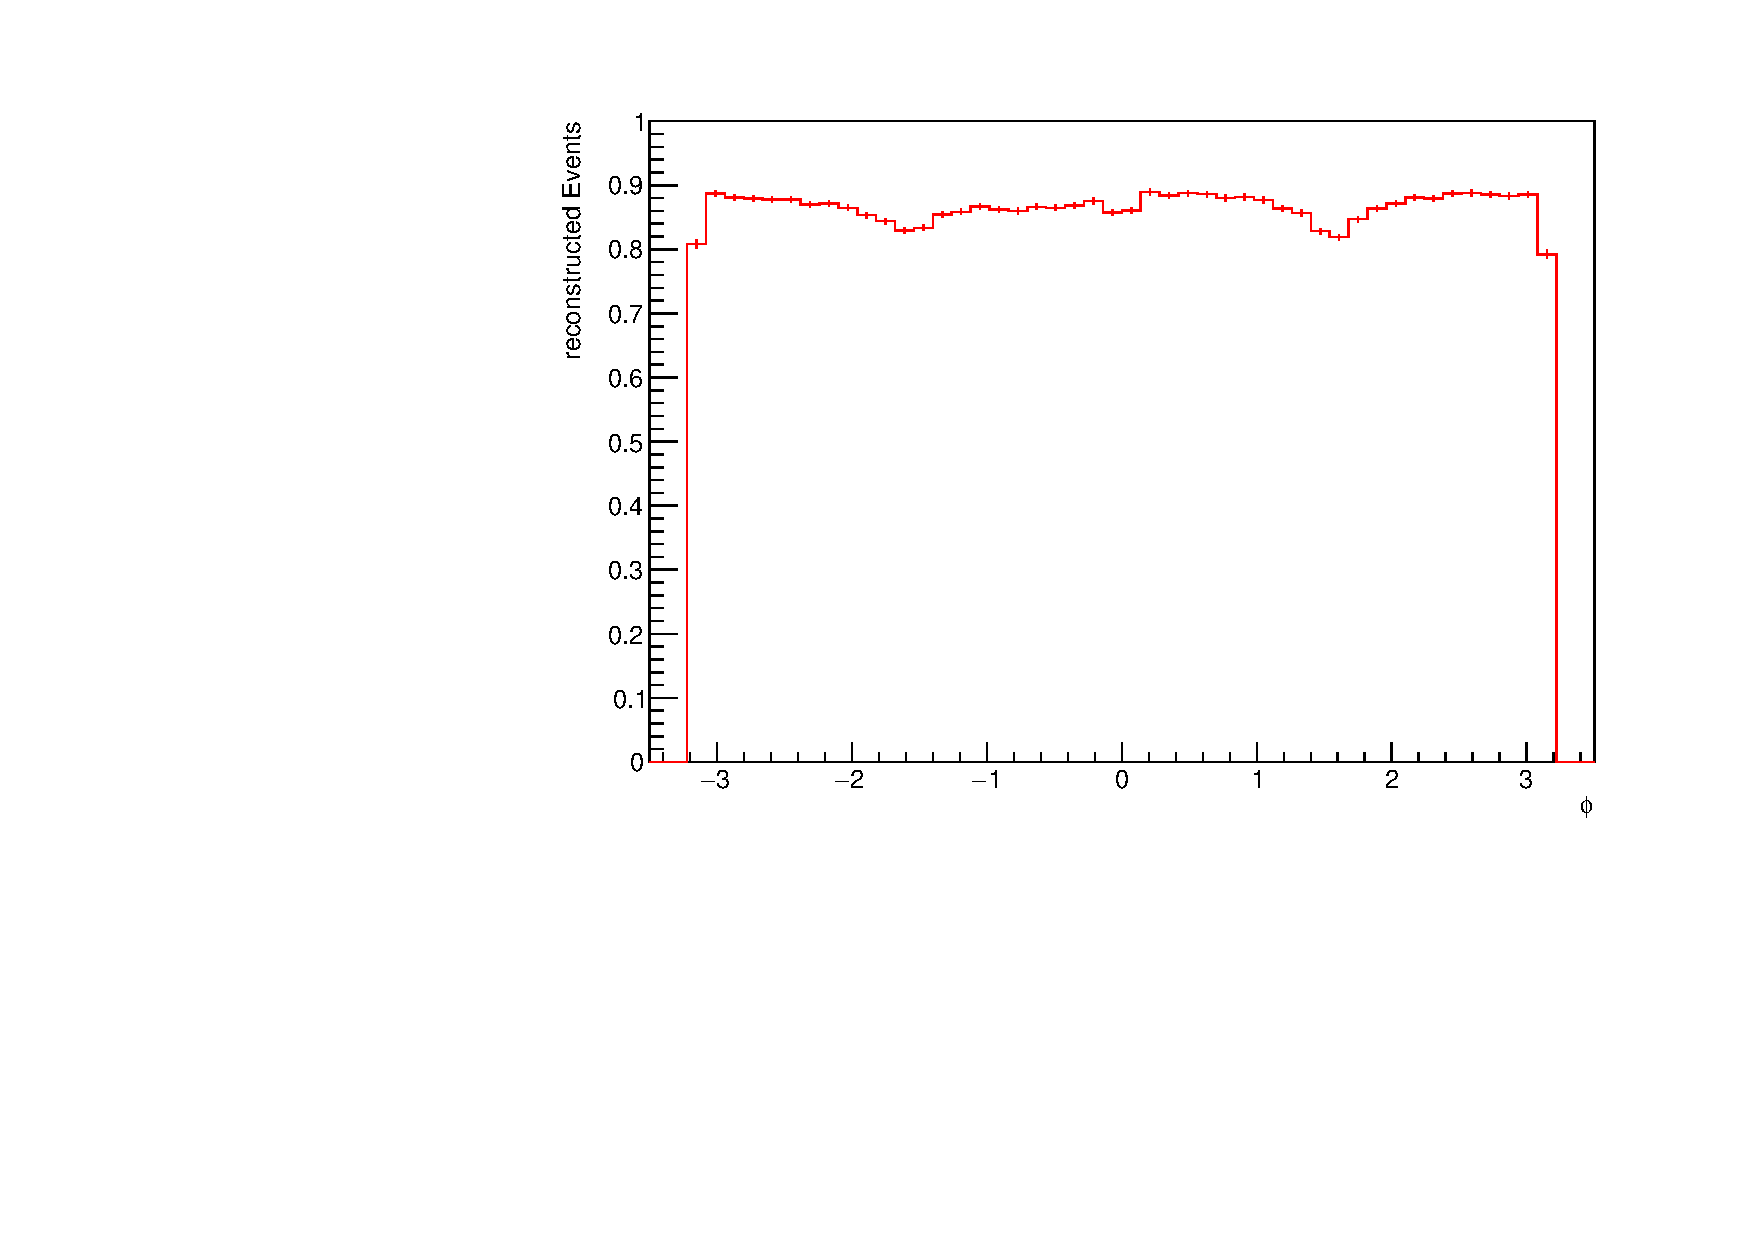
\includegraphics[width=0.9\textwidth]{up_pdf/single/pos/h_phi_reco_Pi_pos.pdf}
\end{subfigure}
\begin{subfigure}{0.45\textwidth}
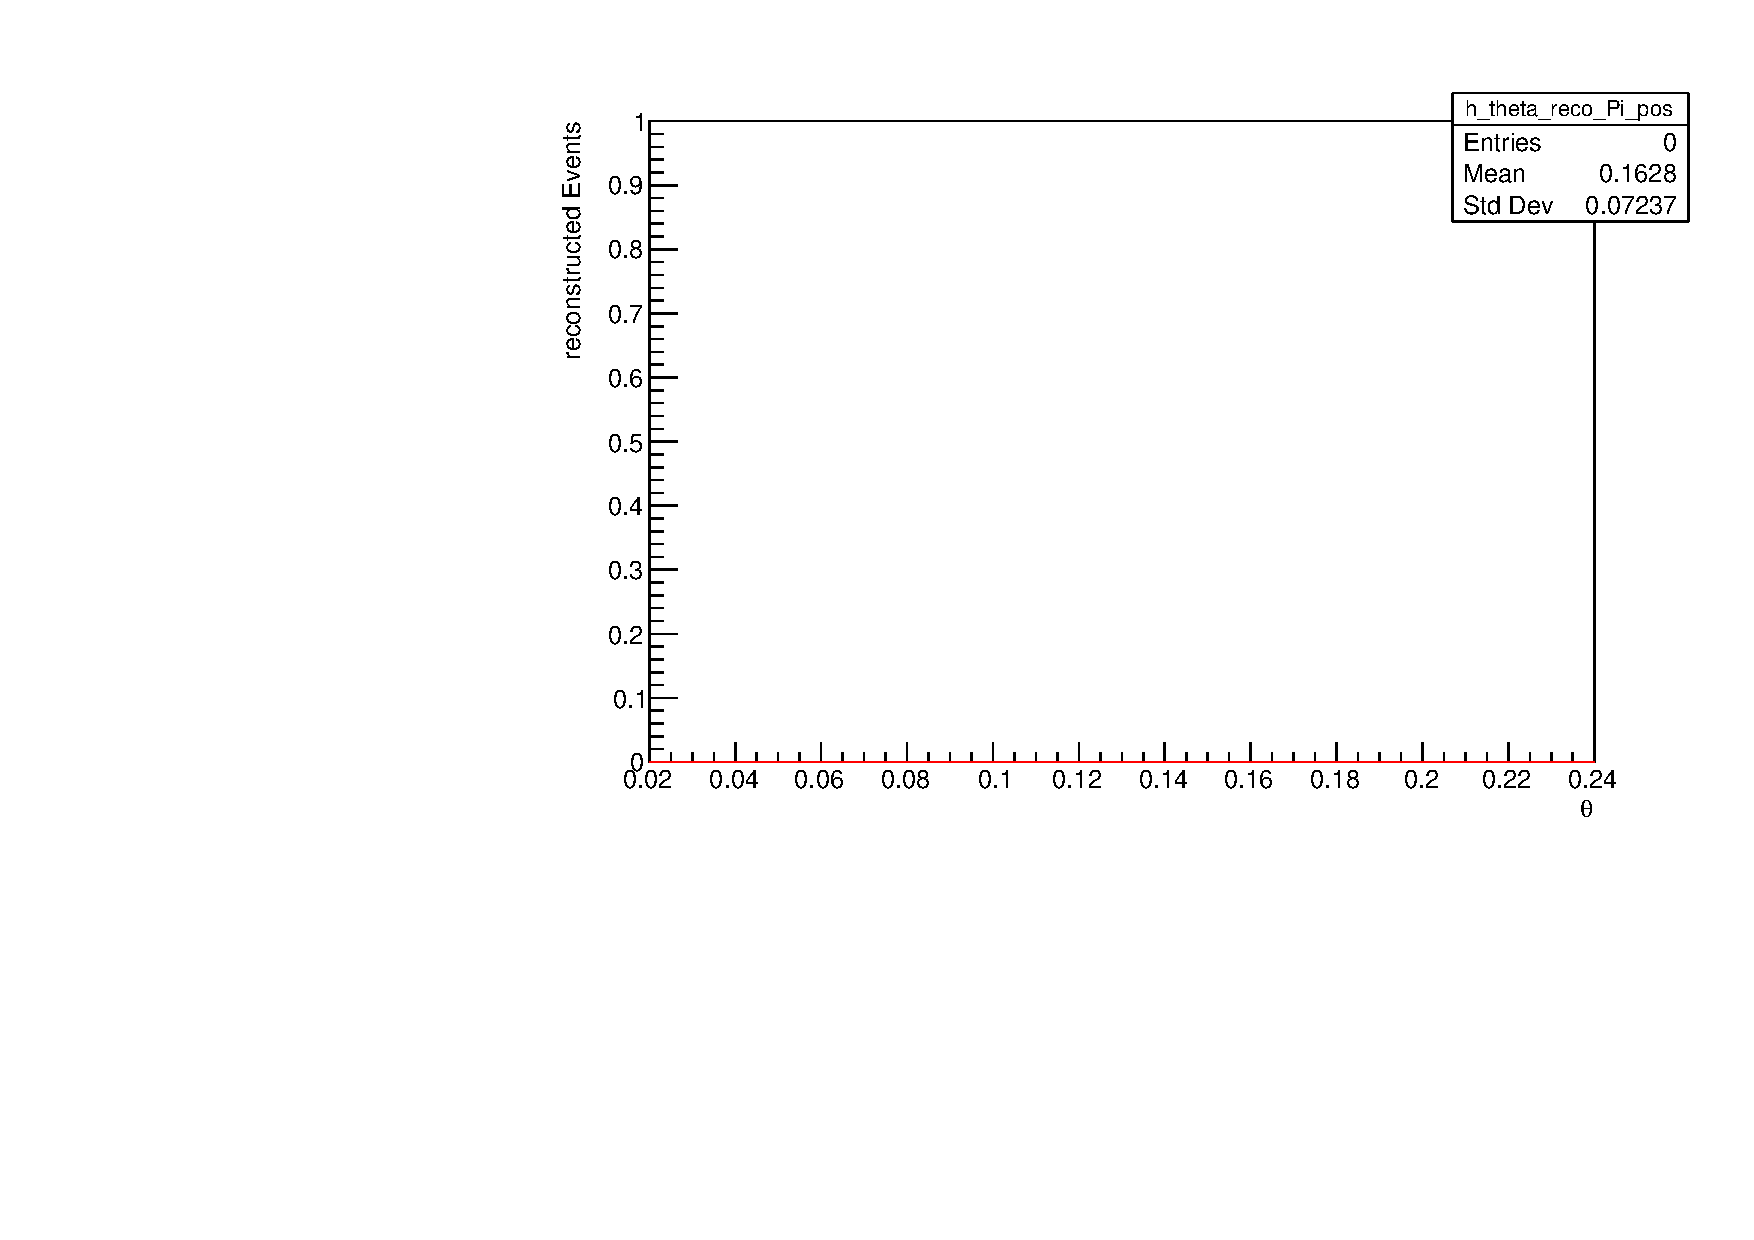
\includegraphics[width=0.9\textwidth]{up_pdf/single/pos/h_theta_reco_Pi_pos.pdf}
\end{subfigure}
\begin{subfigure}{0.45\textwidth}
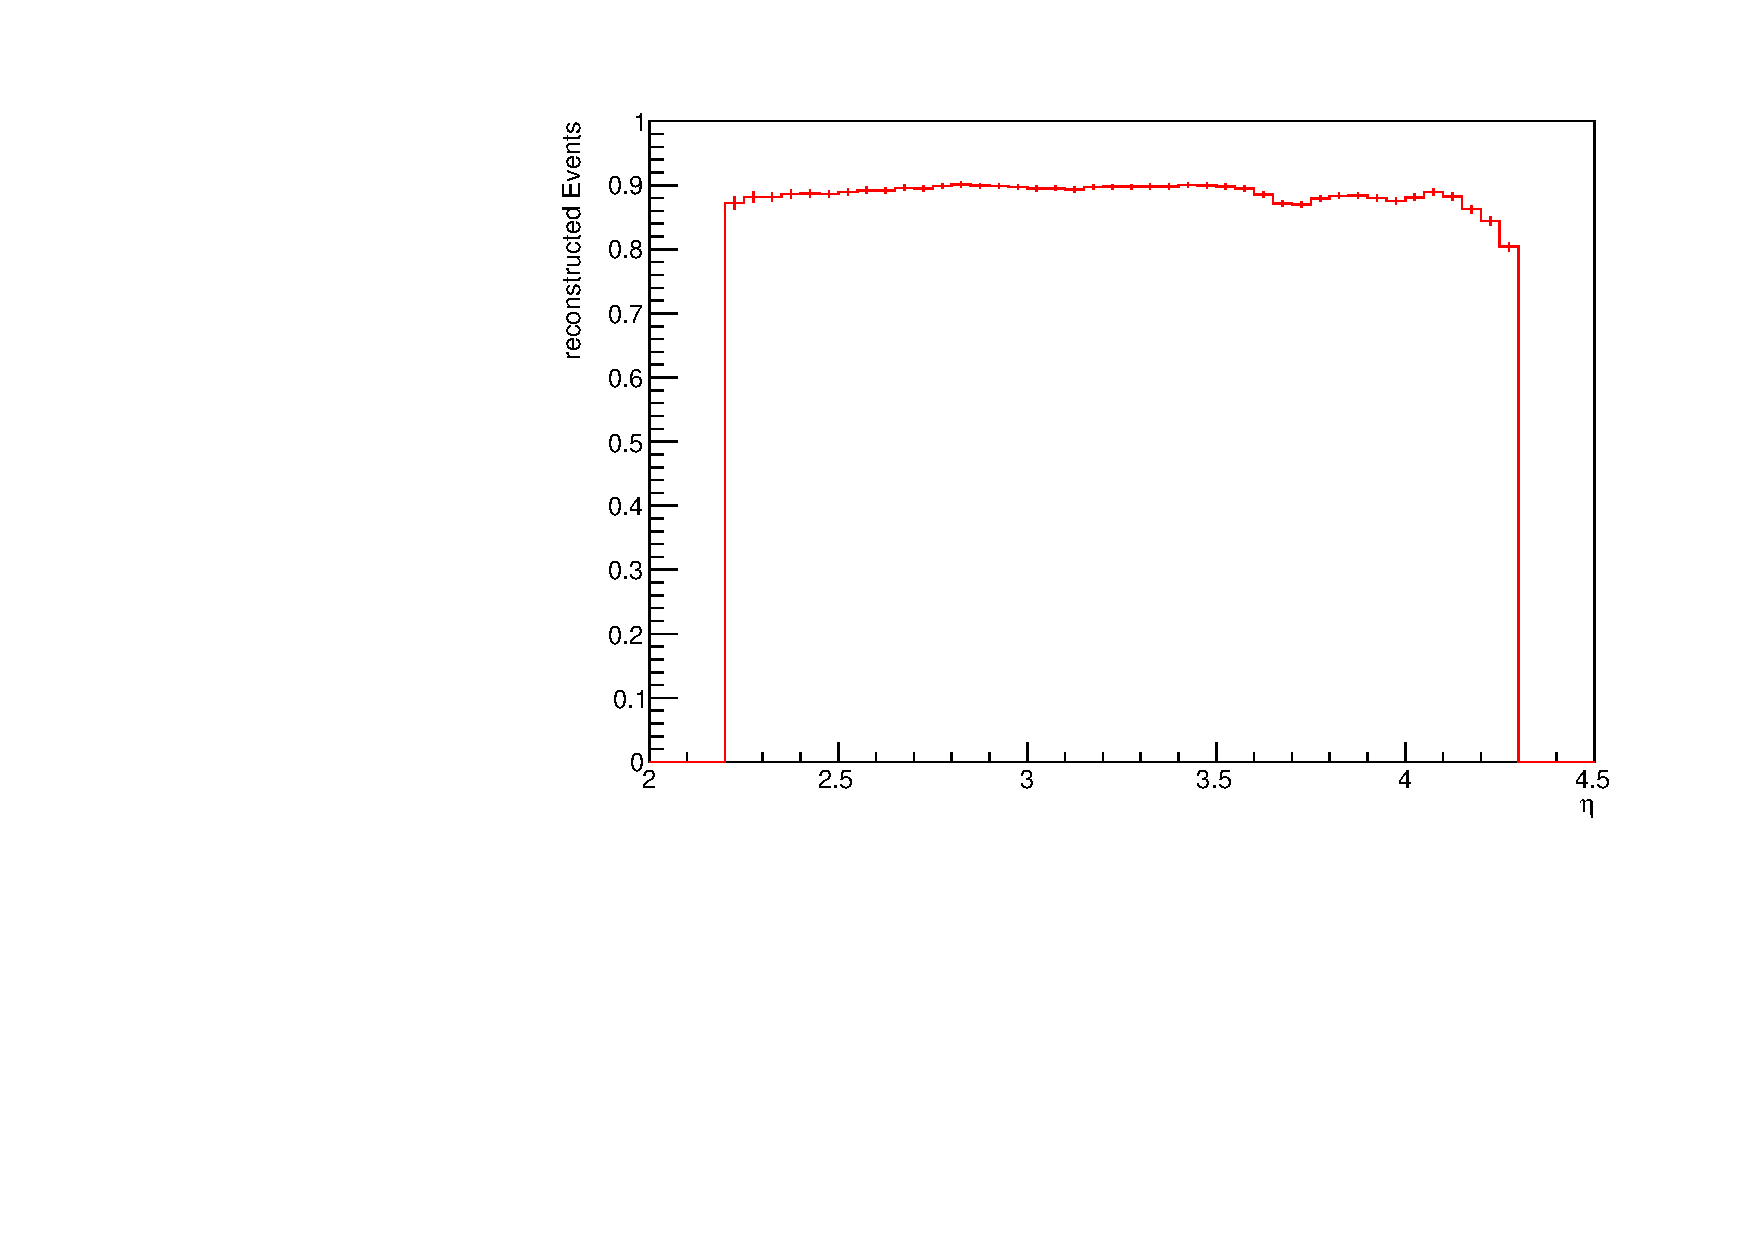
\includegraphics[width=0.9\textwidth]{up_pdf/single/pos/h_eta_reco_Pi_pos.pdf}
\end{subfigure}
\end{figure}
\end{frame}
\begin{frame}{$K$-efficiency}
\begin{figure}
\begin{subfigure}{0.45\textwidth}
\includegraphics[width=0.9\textwidth]{up_pdf/single/pos/h_pt_reco_K_pos.pdf}
\end{subfigure}
\begin{subfigure}{0.45\textwidth}
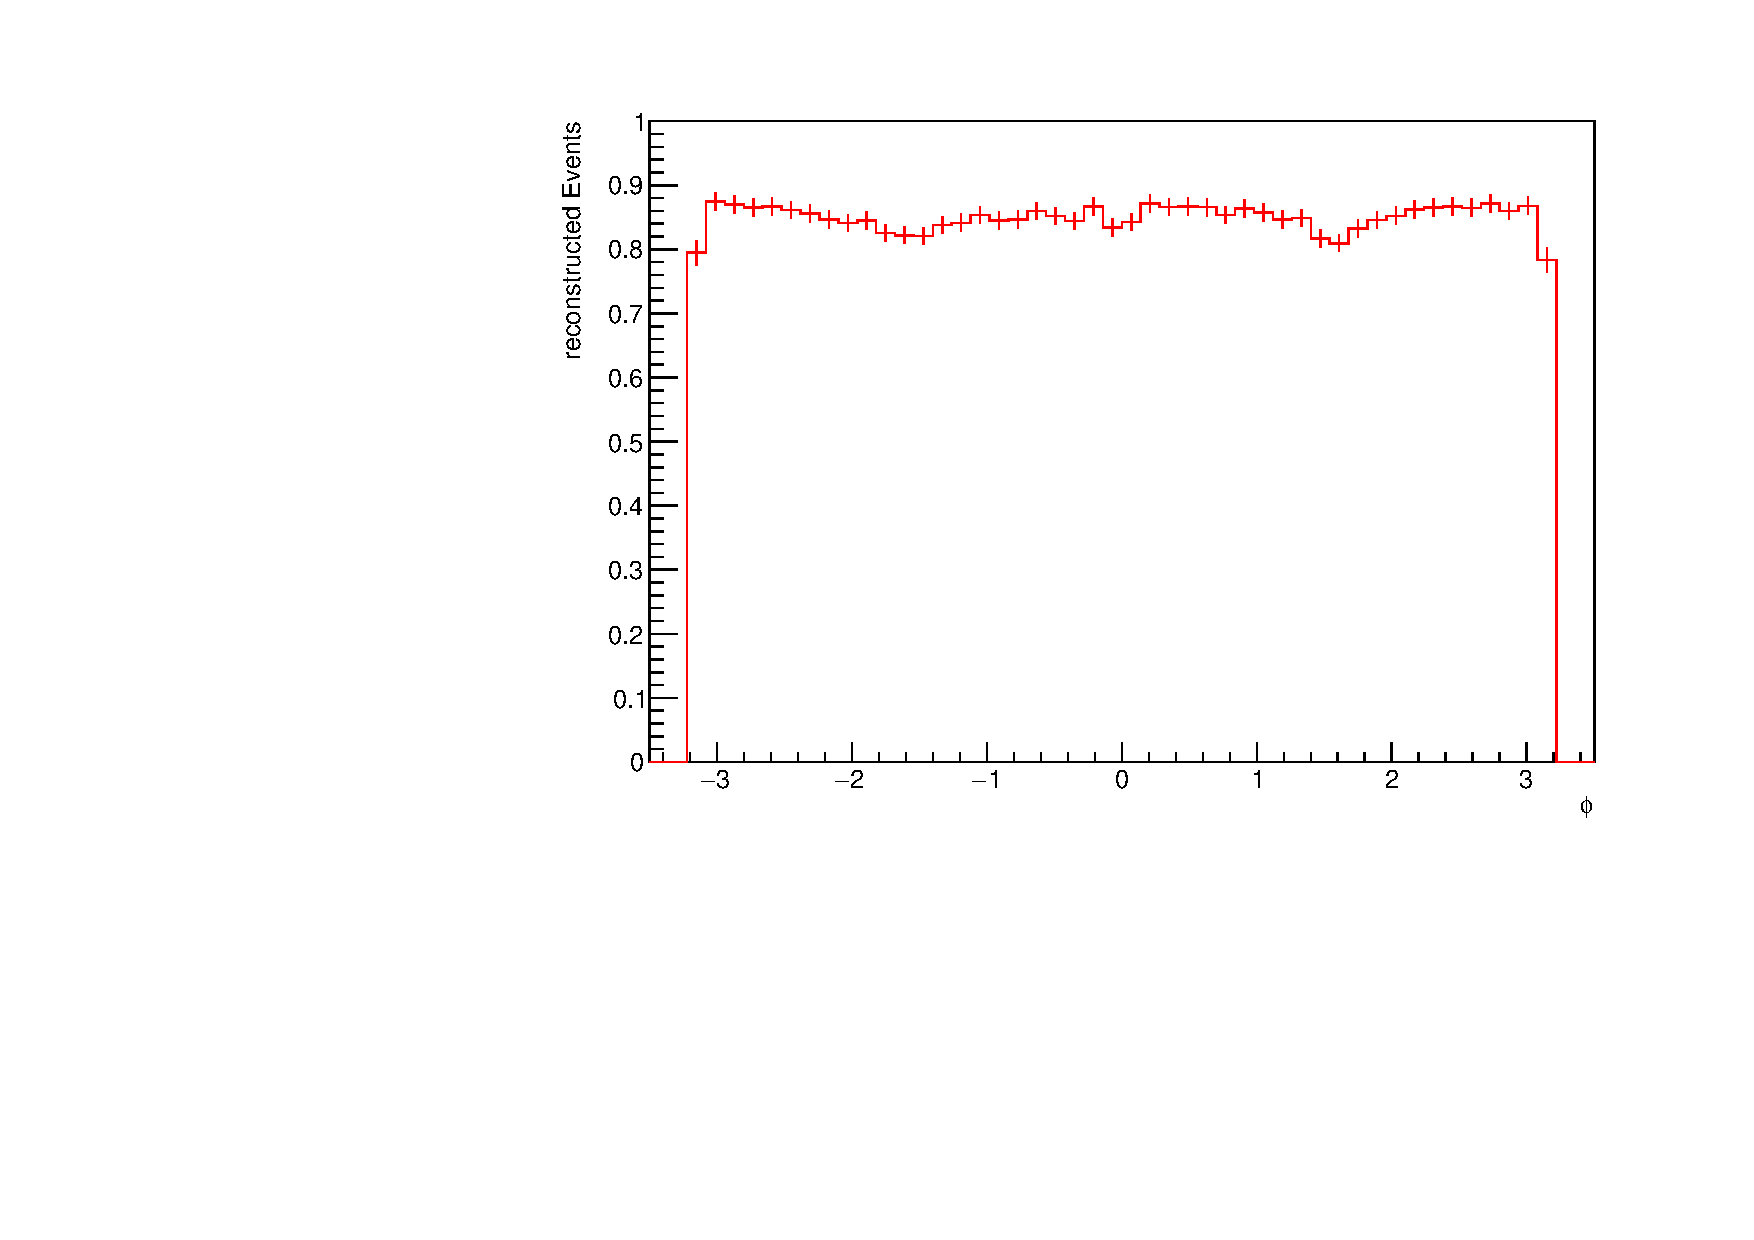
\includegraphics[width=0.9\textwidth]{up_pdf/single/pos/h_phi_reco_K_pos.pdf}
\end{subfigure}
\begin{subfigure}{0.45\textwidth}
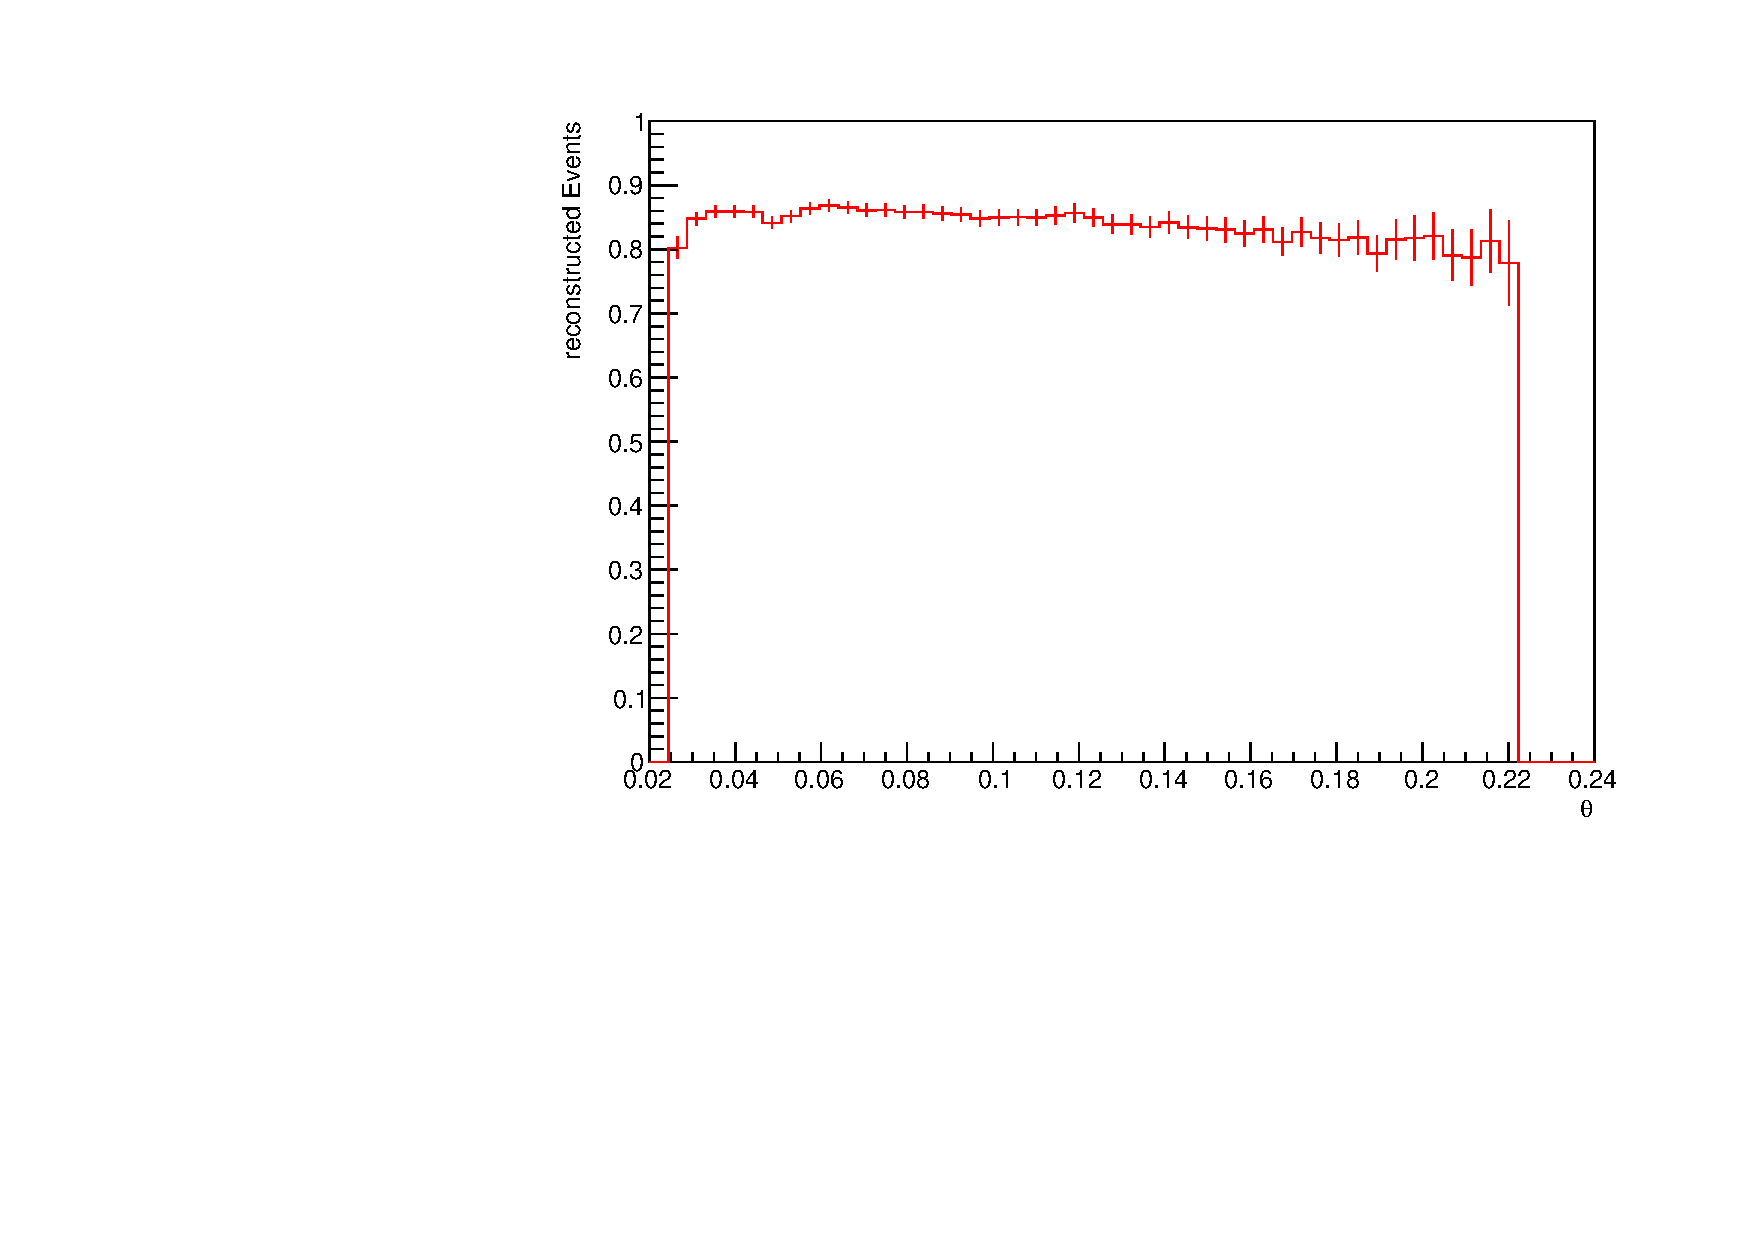
\includegraphics[width=0.9\textwidth]{up_pdf/single/pos/h_theta_reco_K_pos.pdf}
\end{subfigure}
\begin{subfigure}{0.45\textwidth}
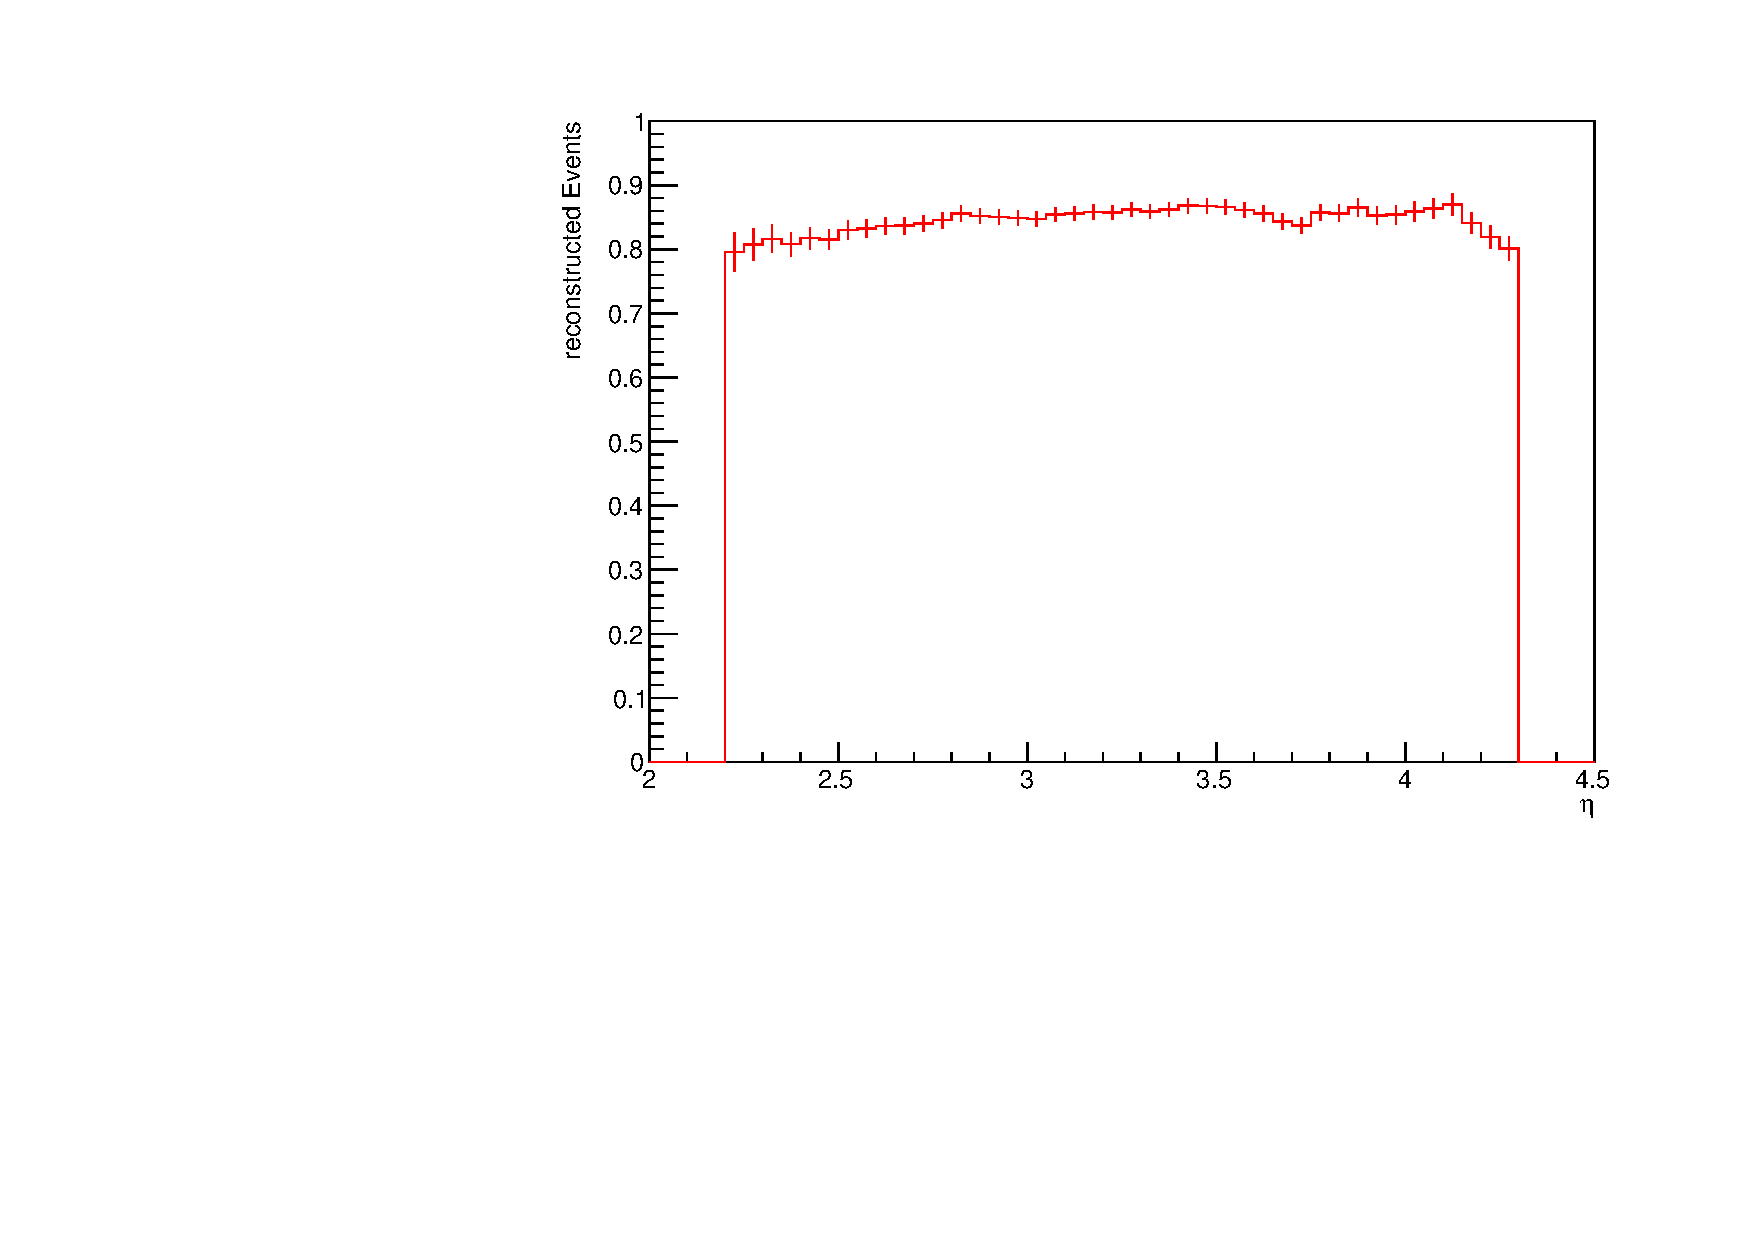
\includegraphics[width=0.9\textwidth]{up_pdf/single/pos/h_eta_reco_K_pos.pdf}
\end{subfigure}
\end{figure}
\end{frame}
\begin{frame}{soft $\pi$-efficiency}
\begin{figure}
\begin{subfigure}{0.45\textwidth}
\includegraphics[width=0.9\textwidth]{up_pdf/single/pos/h_pt_reco_SPi_pos.pdf}
\end{subfigure}
\begin{subfigure}{0.45\textwidth}
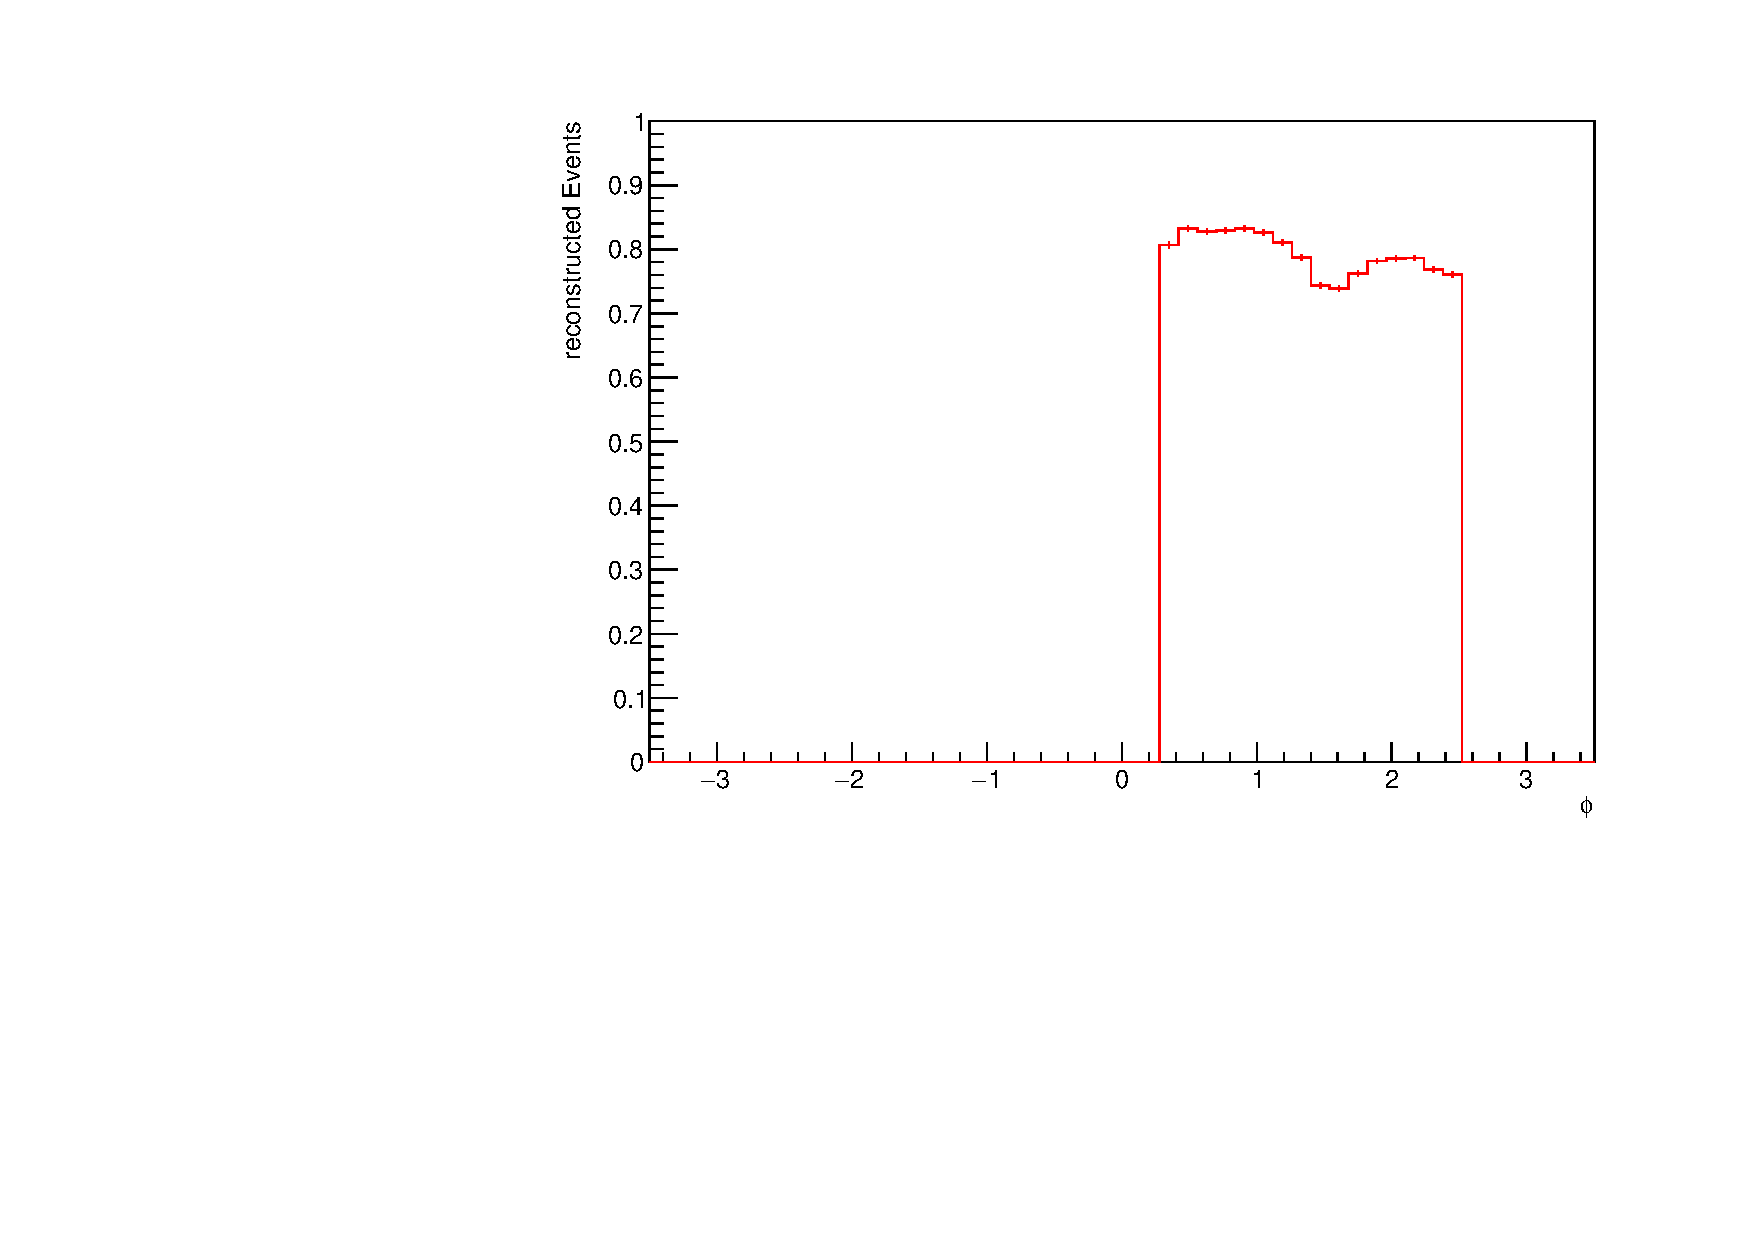
\includegraphics[width=0.9\textwidth]{up_pdf/single/pos/h_phi_reco_SPi_pos.pdf}
\end{subfigure}
\begin{subfigure}{0.45\textwidth}
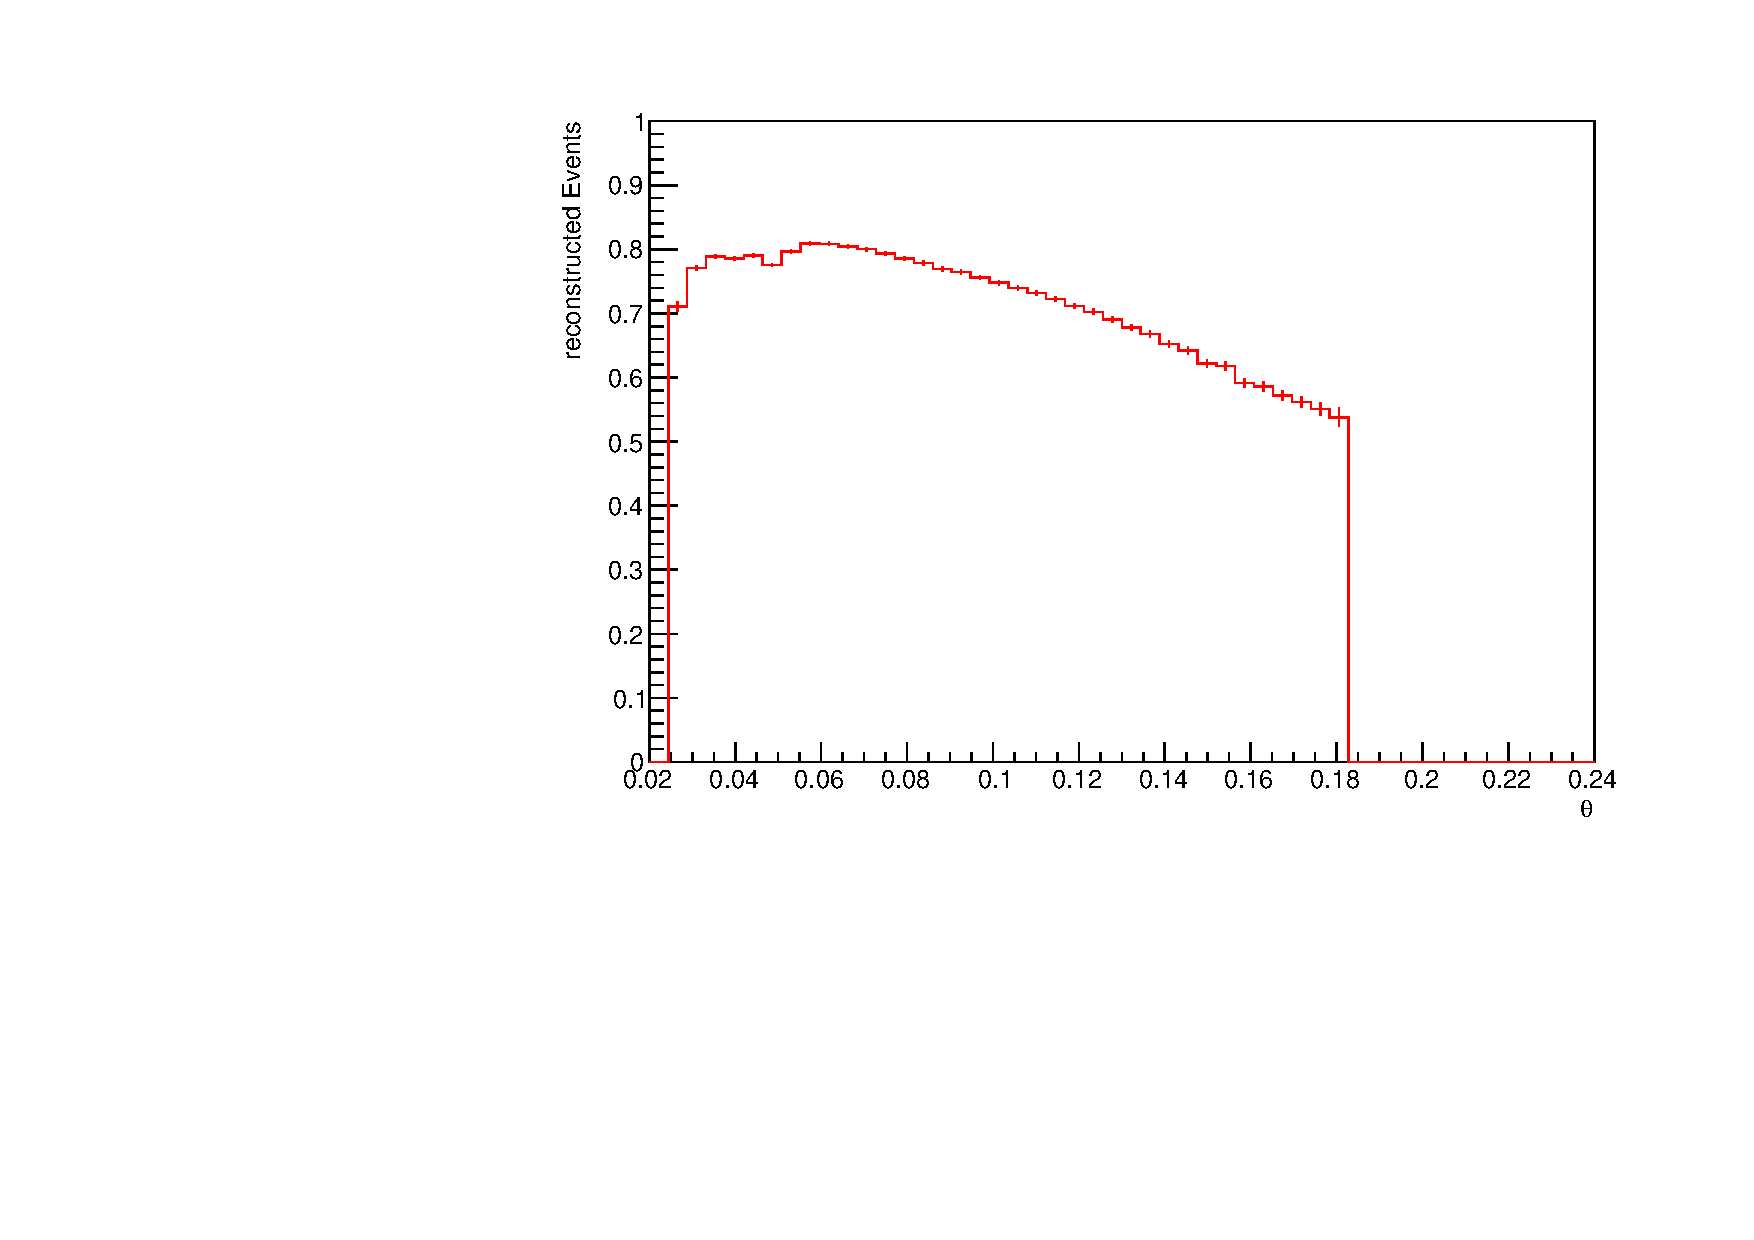
\includegraphics[width=0.9\textwidth]{up_pdf/single/pos/h_theta_reco_SPi_pos.pdf}
\end{subfigure}
\begin{subfigure}{0.45\textwidth}
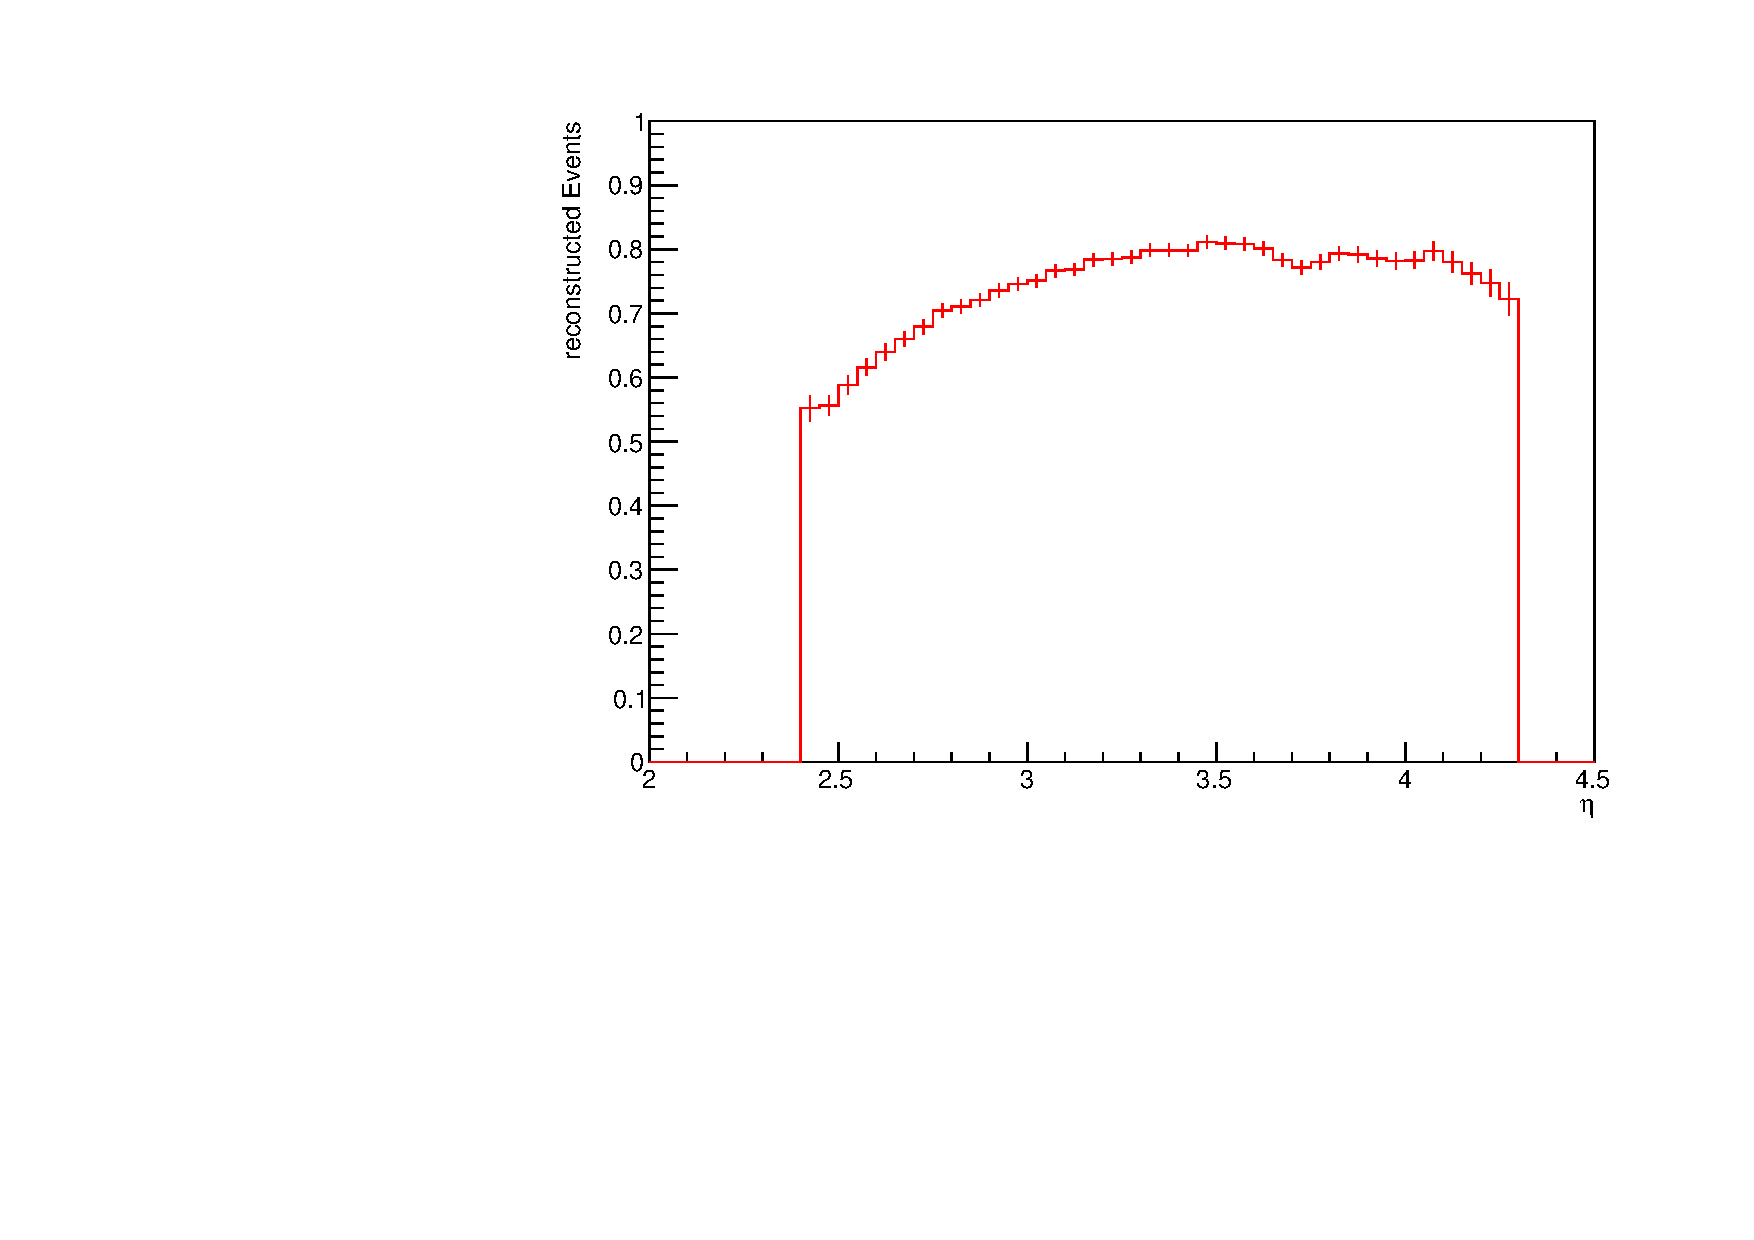
\includegraphics[width=0.9\textwidth]{up_pdf/single/pos/h_eta_reco_SPi_pos.pdf}
\end{subfigure}
\end{figure}
\end{frame}
\begin{frame}{$D^0$-efficiency}
\begin{figure}
\begin{subfigure}{0.45\textwidth}
\includegraphics[width=0.9\textwidth]{up_pdf/single/pos/h_pt_reco_D0_pos.pdf}
\end{subfigure}
\begin{subfigure}{0.45\textwidth}
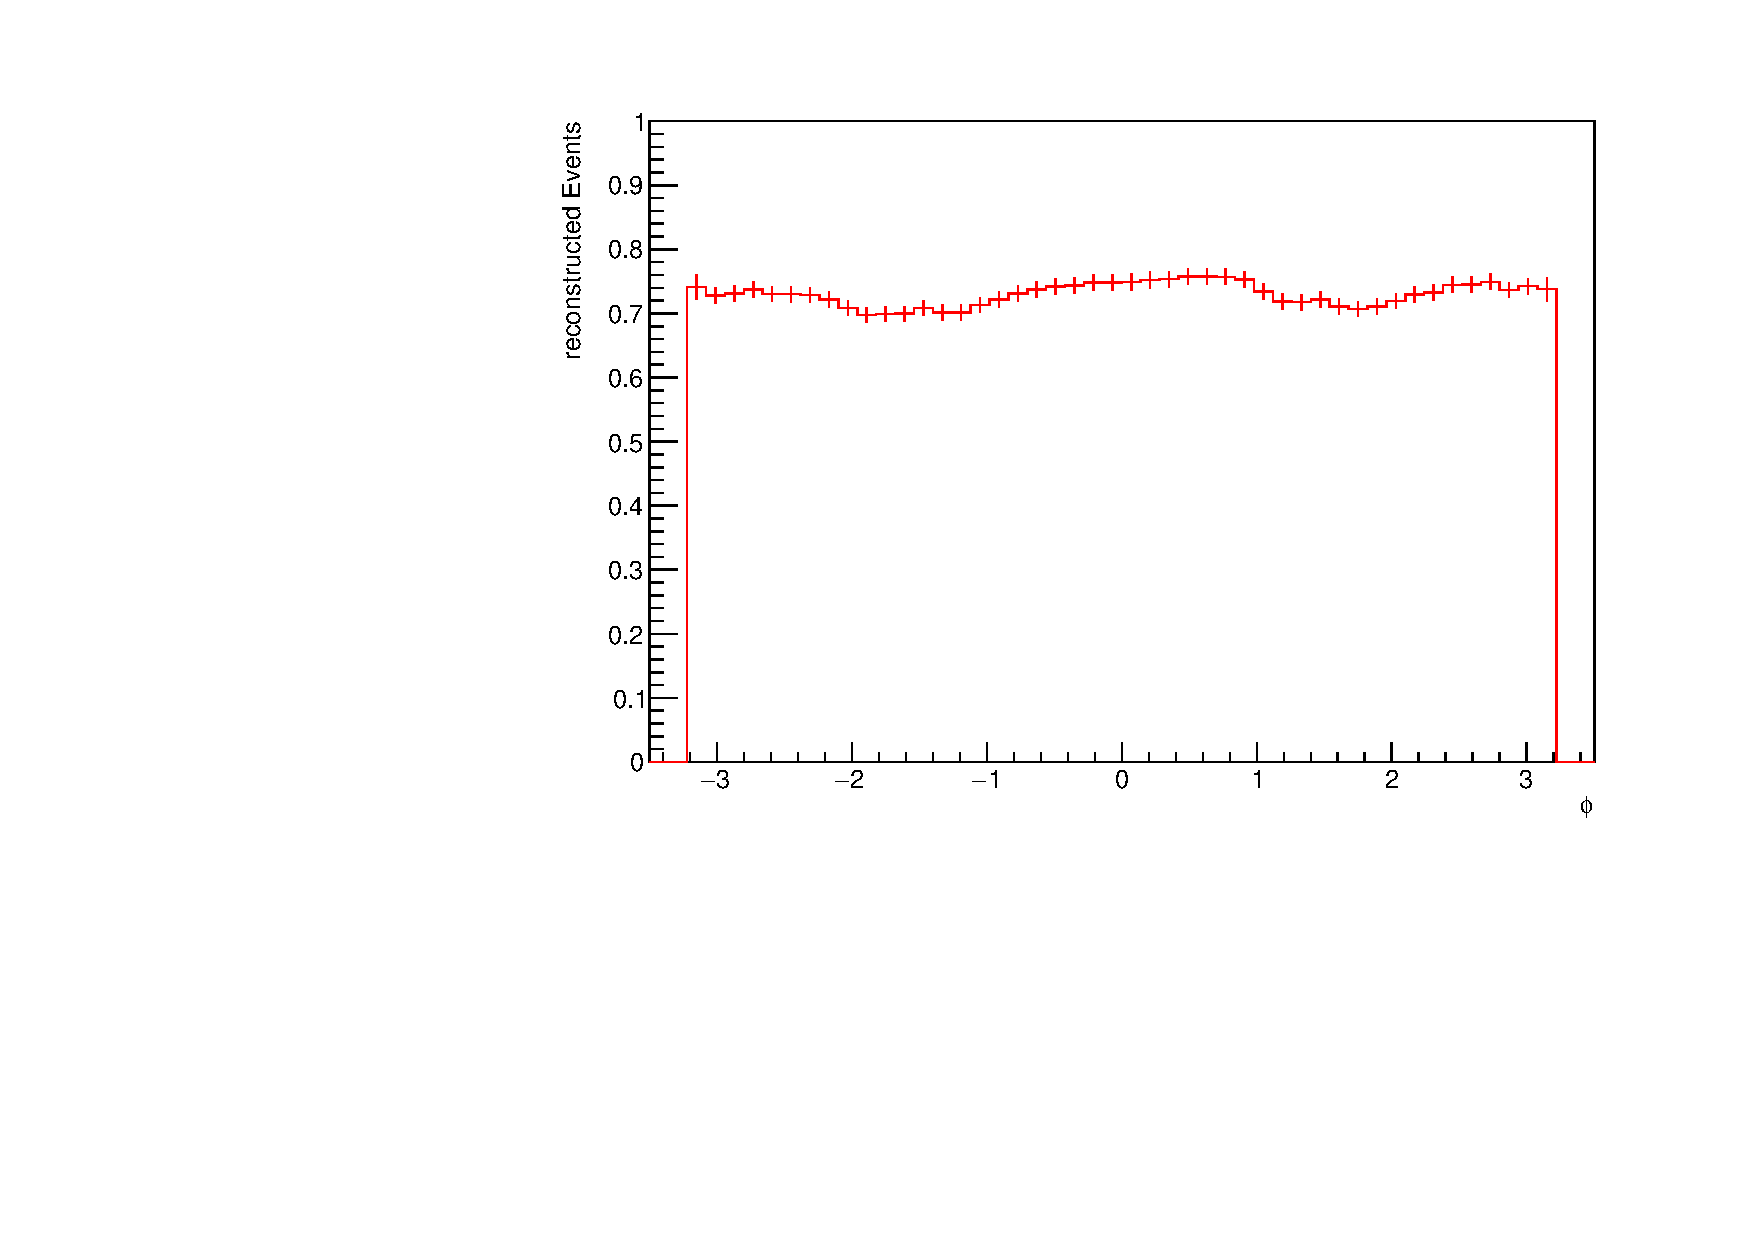
\includegraphics[width=0.9\textwidth]{up_pdf/single/pos/h_phi_reco_D0_pos.pdf}
\end{subfigure}
\begin{subfigure}{0.45\textwidth}
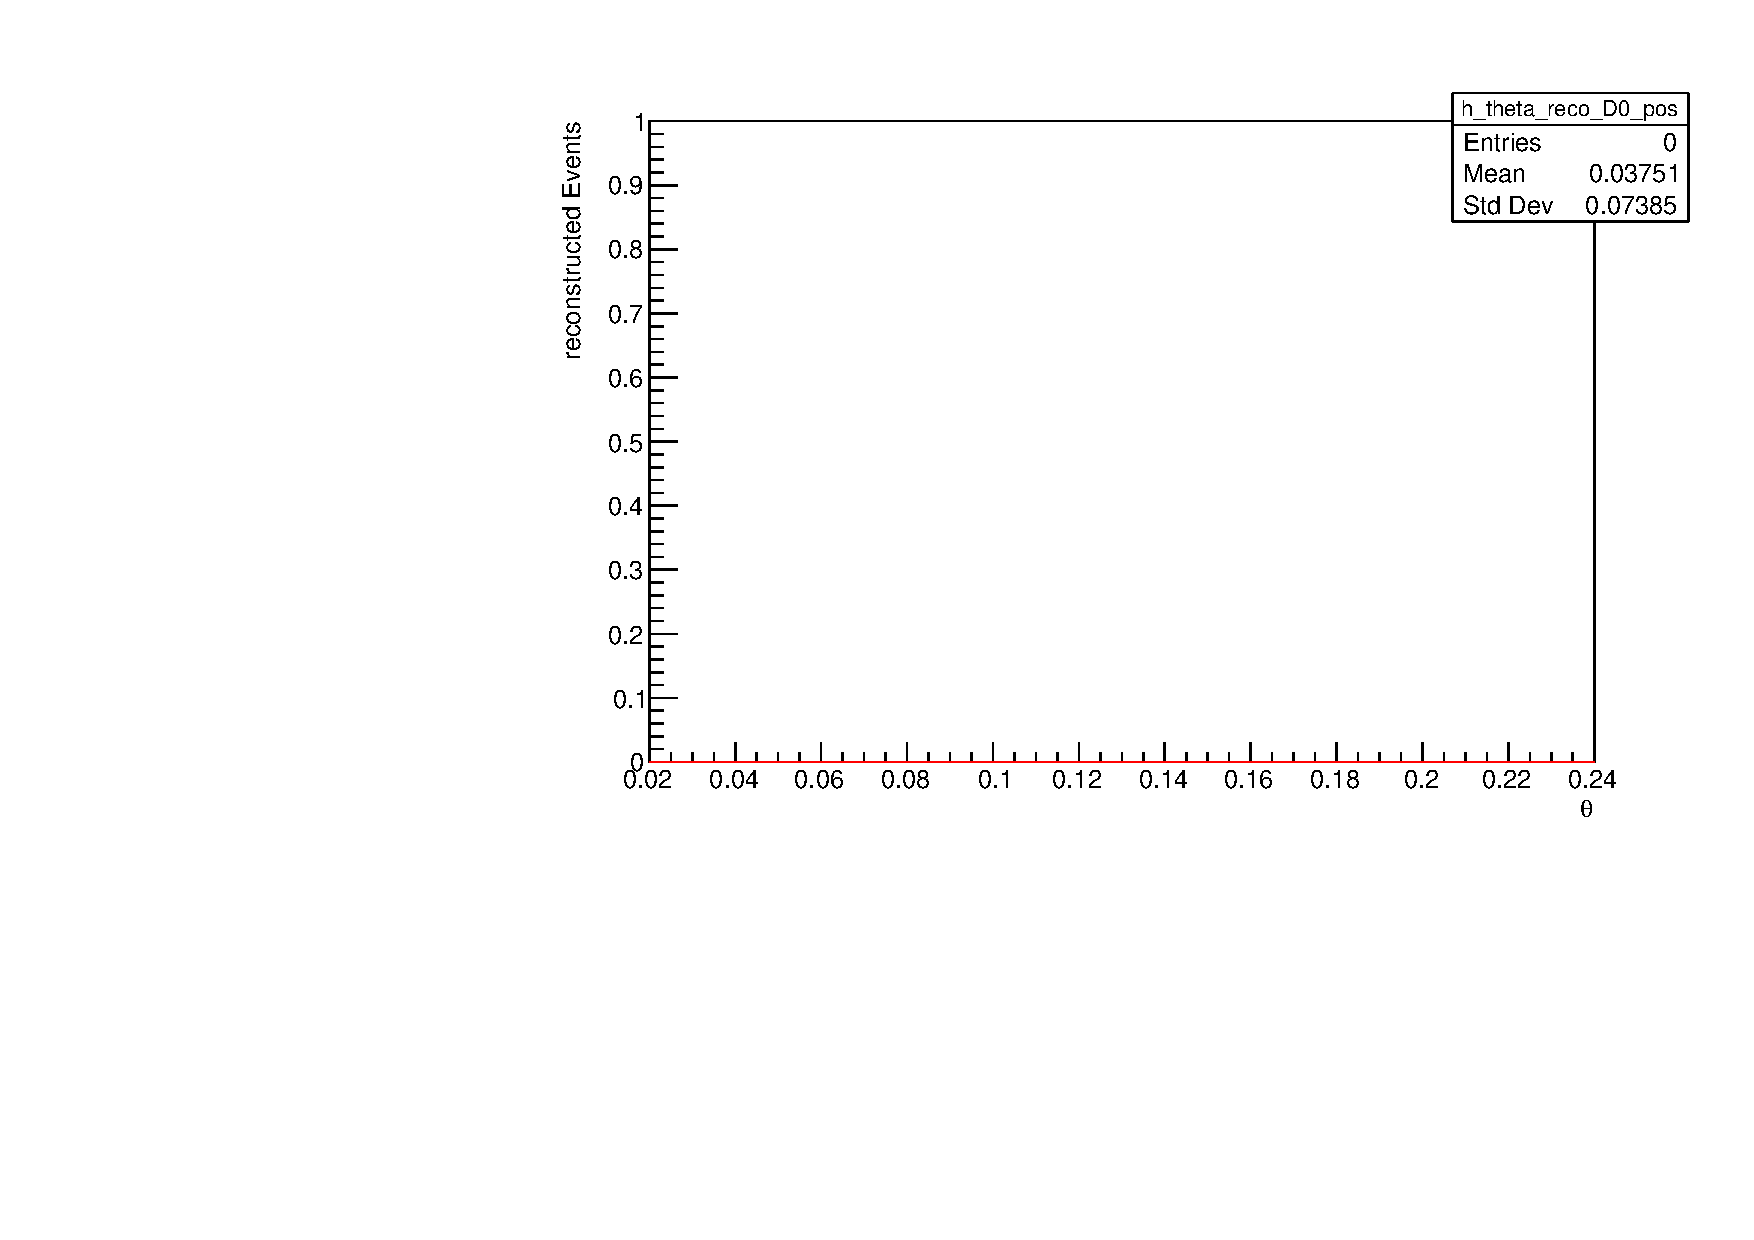
\includegraphics[width=0.9\textwidth]{up_pdf/single/pos/h_theta_reco_D0_pos.pdf}
\end{subfigure}
\begin{subfigure}{0.45\textwidth}
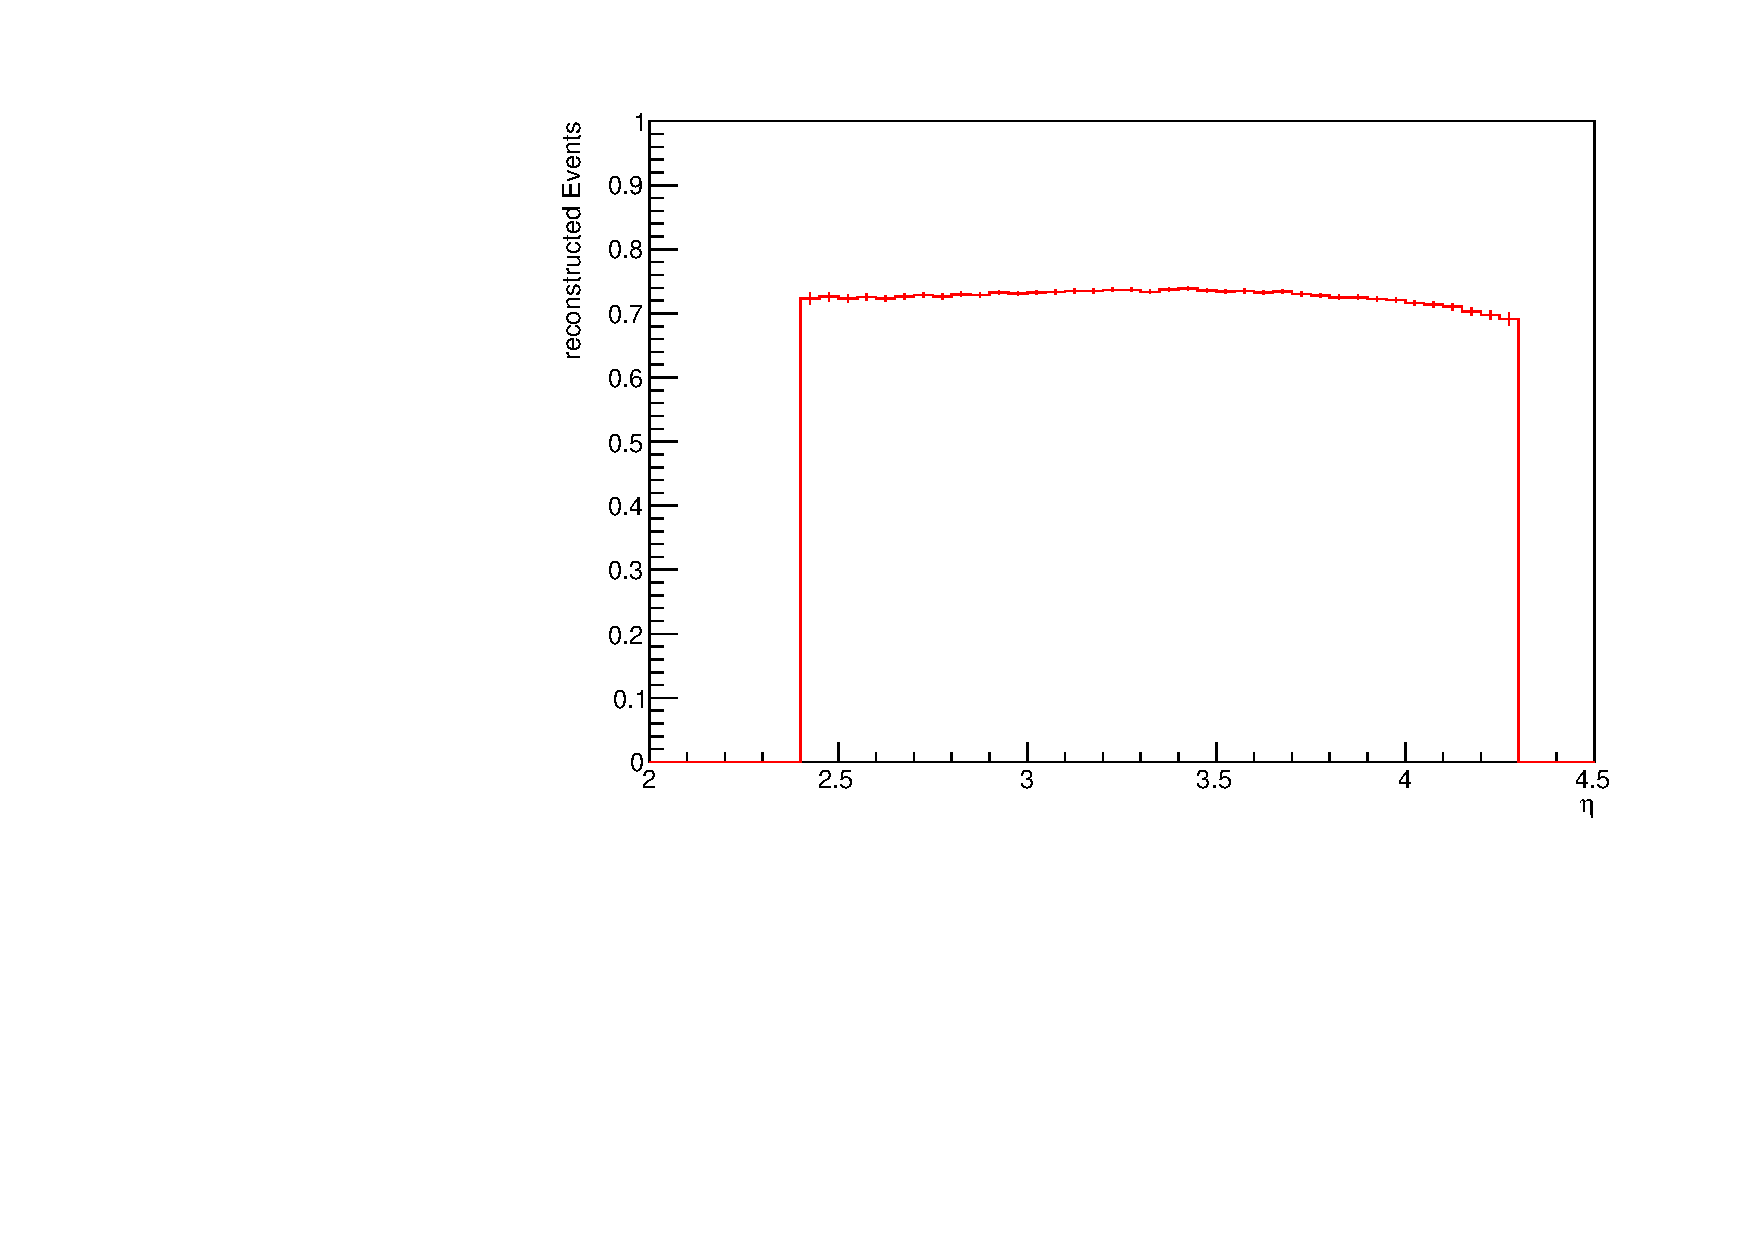
\includegraphics[width=0.9\textwidth]{up_pdf/single/pos/h_eta_reco_D0_pos.pdf}
\end{subfigure}
\end{figure}
\end{frame}
\begin{frame}{$D^*$-efficiency}
\begin{figure}
\begin{subfigure}{0.45\textwidth}
\includegraphics[width=0.9\textwidth]{up_pdf/single/pos/h_pt_reco_Dst_pos.pdf}
\end{subfigure}
\begin{subfigure}{0.45\textwidth}
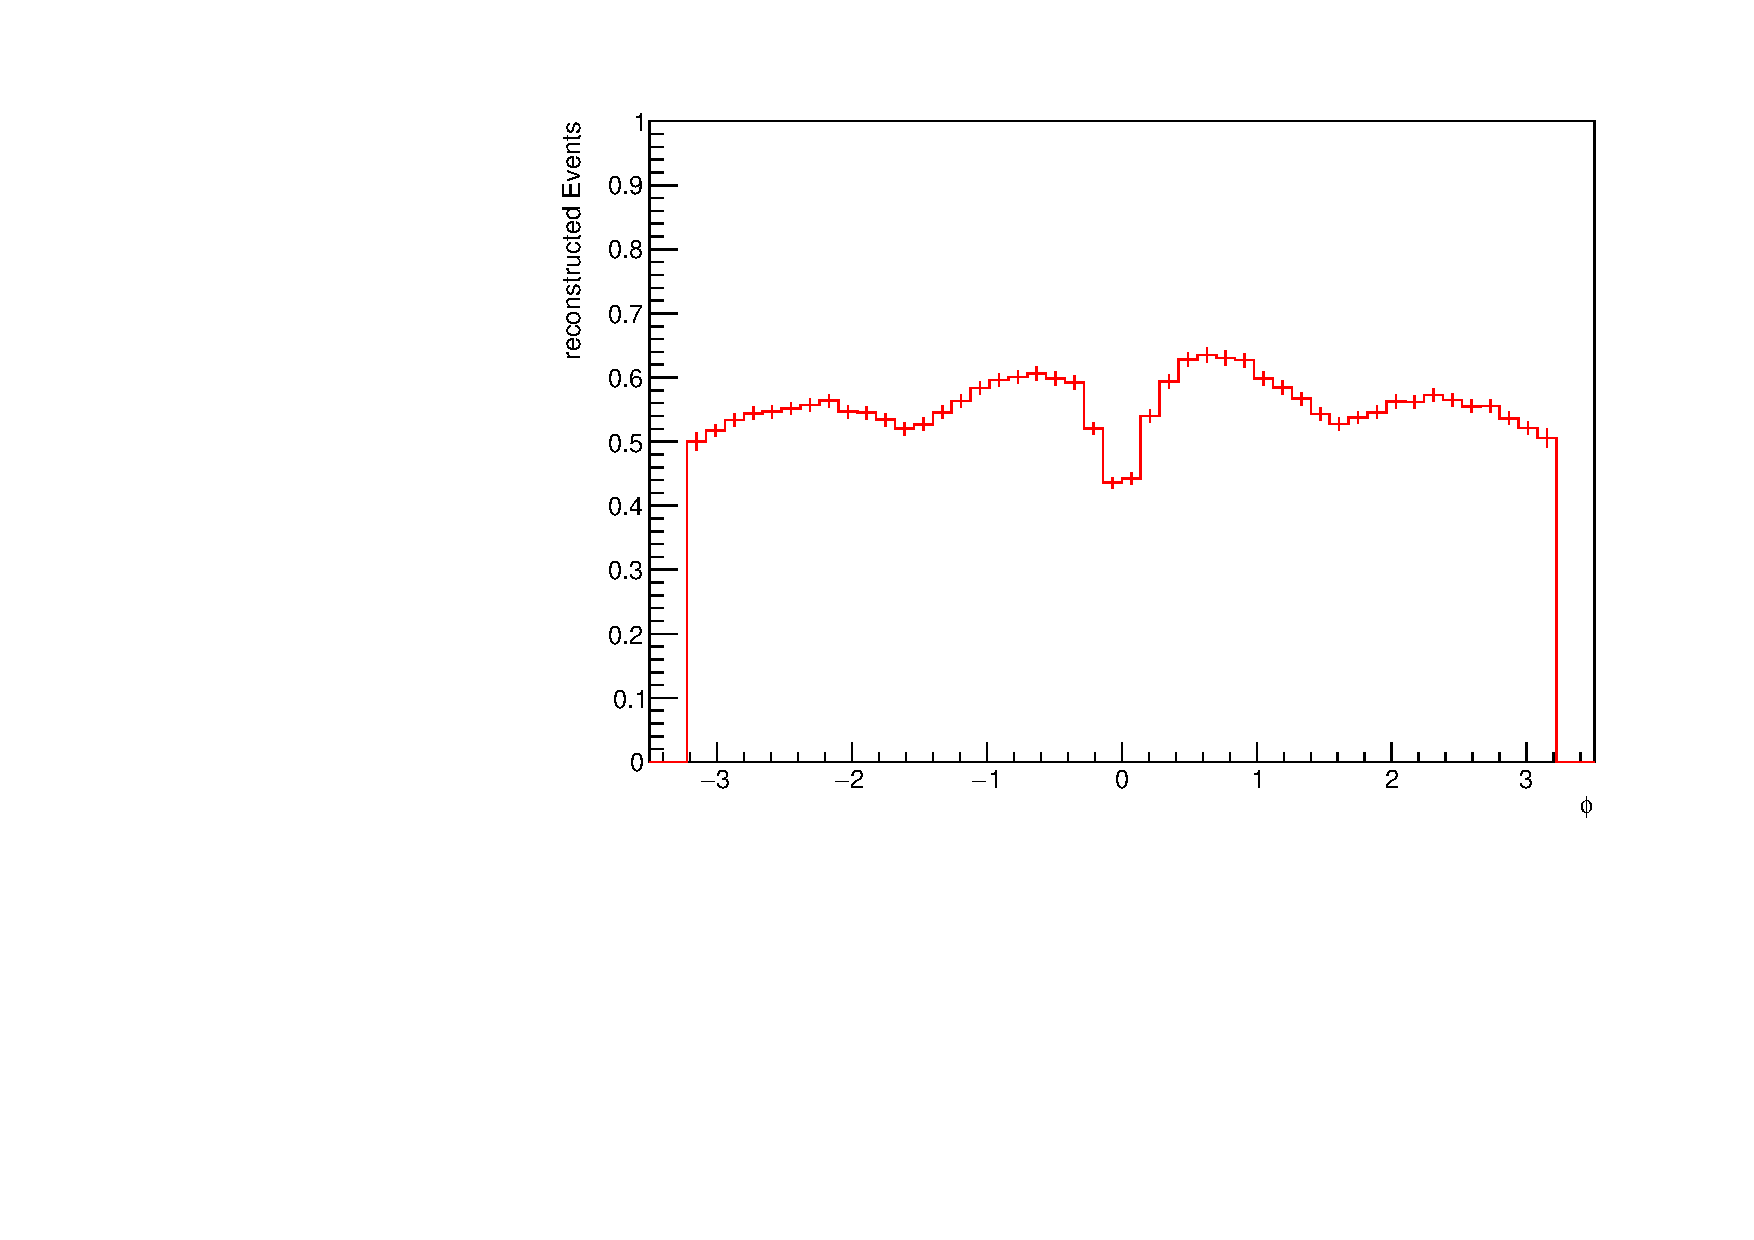
\includegraphics[width=0.9\textwidth]{up_pdf/single/pos/h_phi_reco_Dst_pos.pdf}
\end{subfigure}
\begin{subfigure}{0.45\textwidth}
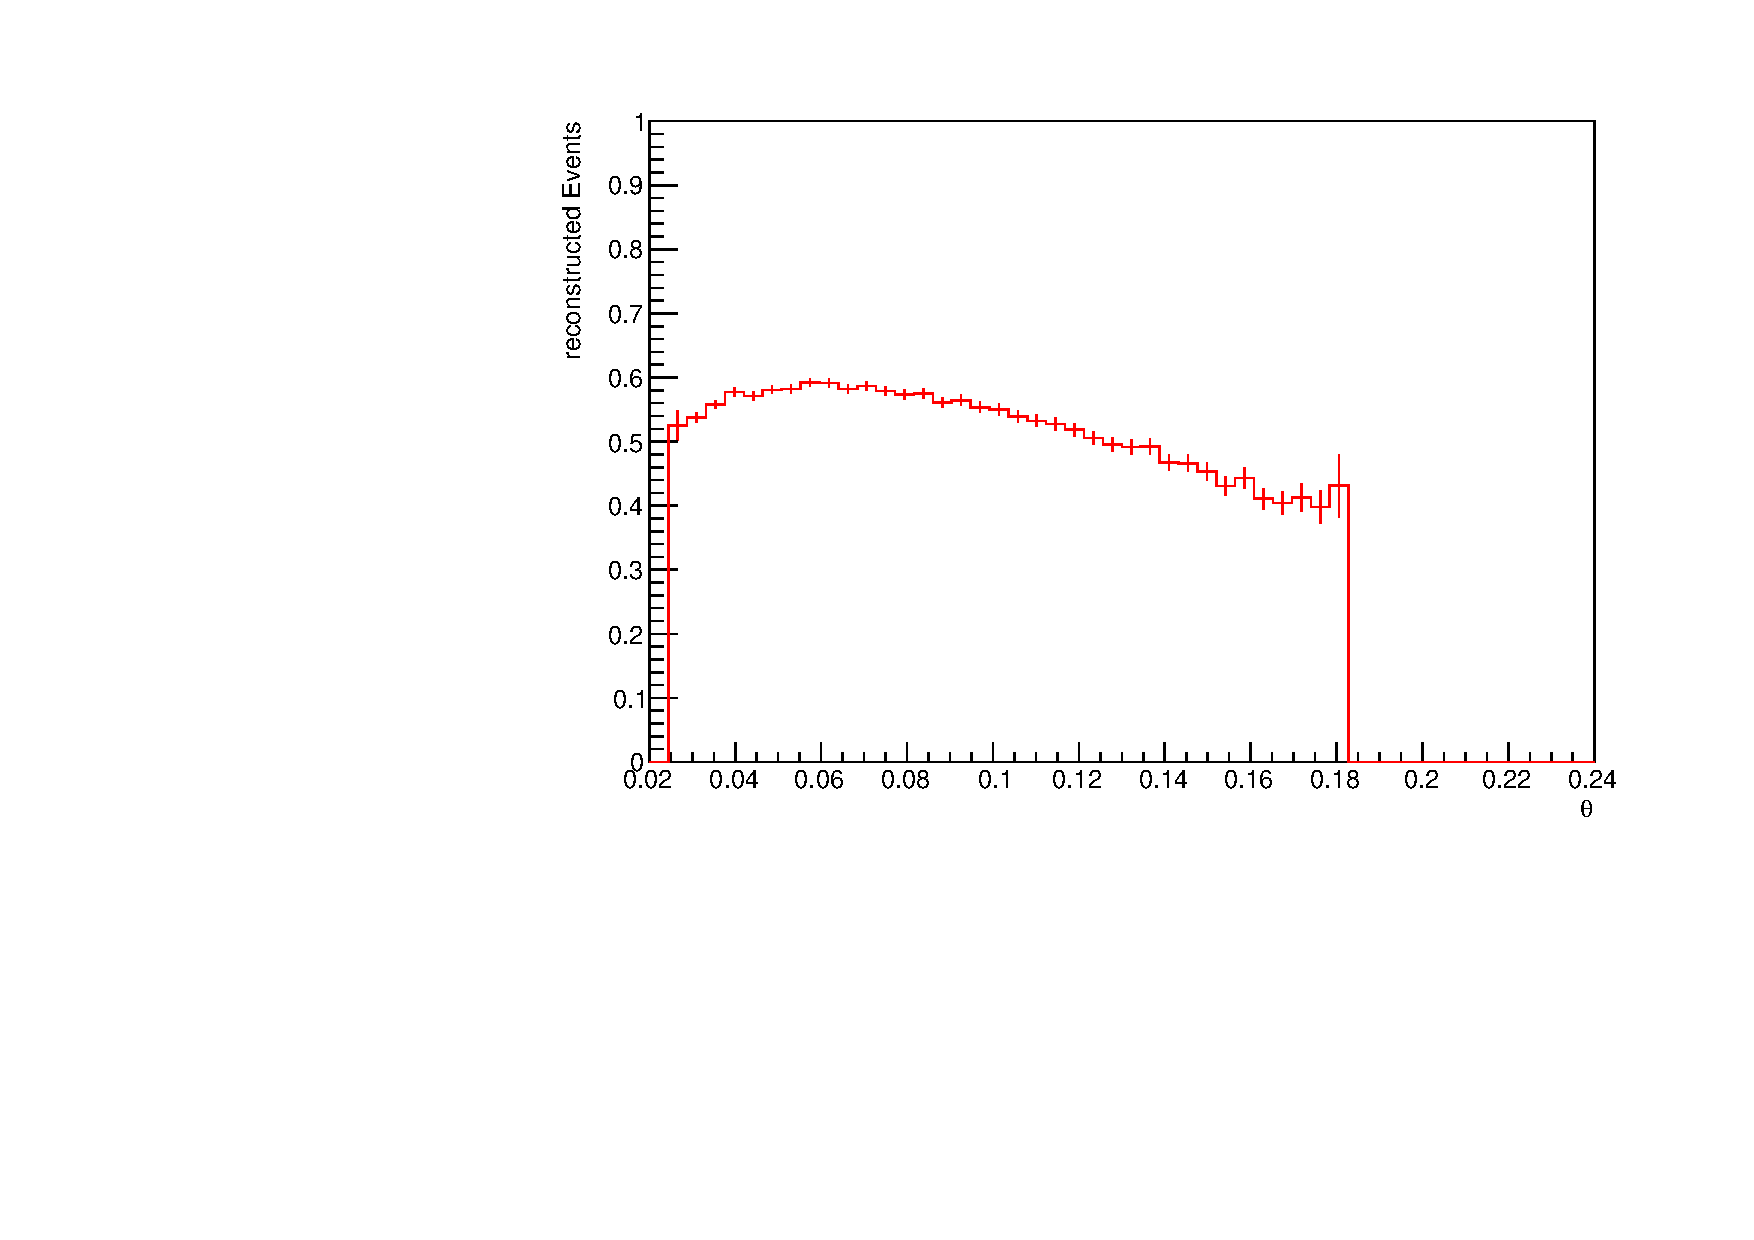
\includegraphics[width=0.9\textwidth]{up_pdf/single/pos/h_theta_reco_Dst_pos.pdf}
\end{subfigure}
\begin{subfigure}{0.45\textwidth}
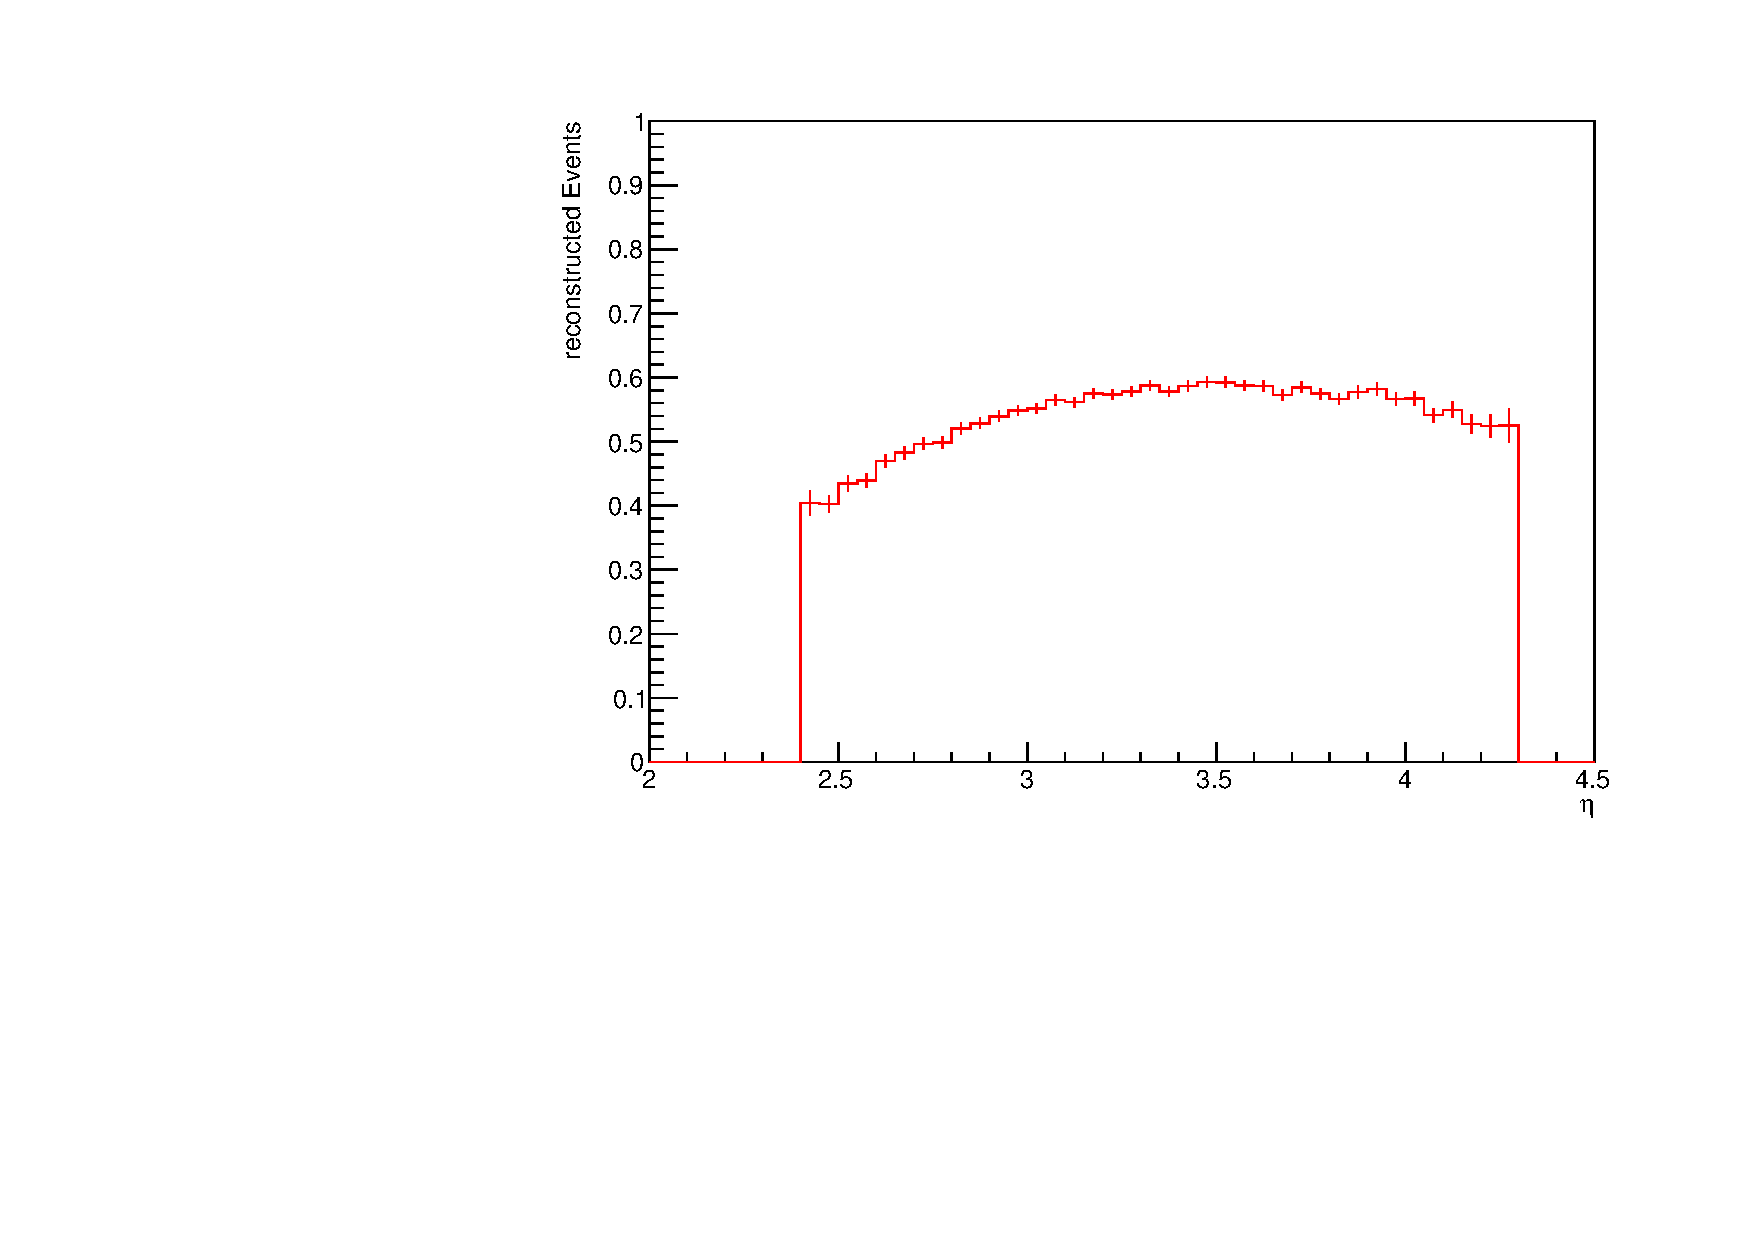
\includegraphics[width=0.9\textwidth]{up_pdf/single/pos/h_eta_reco_Dst_pos.pdf}
\end{subfigure}
\end{figure}
\end{frame}
\begin{frame}
\begin{LARGE}
\textbf{Charge: -}
\end{LARGE}
\end{frame}
\begin{frame}{Efficiencies}
\begin{table}
%\caption{Reconstruction efficiencies for different polarities}
\resizebox{\textwidth}{!}{
	\begin{tabular}{cS[table-format=2.2]@{${}\pm{}$}S[table-format=1.2]S[table-format=2.2]@{${}\pm{}$}S[table-format=1.2]S[table-format=2.2]@{${}\pm{}$}S[table-format=1.2]S[table-format=2.2]@{${}\pm{}$}S[table-format=1.2]S[table-format=2.2]@{${}\pm{}$}S[table-format=1.2]}
		\toprule
		{Polarity} & \multicolumn{2}{c}{$\epsilon_{\pi} $} & \multicolumn{2}{c}{$\epsilon_{K} $} & \multicolumn{2}{c}{$ \epsilon_{\pi,s} $} & \multicolumn{2}{c}{$\epsilon_{D^0} $} & \multicolumn{2}{c}{$\epsilon_{D^*} $} \\
		\midrule
		$UP$ & 86.65 & 0.02 & 84.25 & 0.02 & 76.93 & 0.02 & 73.67 & 0.03 & 56.76 & 0.03 \\
		$DOWN$ & 86.66 & 0.02 & 84.27 & 0.02 & 76.34 & 0.02 & 73.72 & 0.03 & 56.36 & 0.02 \\
		\bottomrule
	\end{tabular}}
%\caption{UP Polarity - reconstructed vs. total number of events}
\resizebox{\textwidth}{!}{
	\begin{tabular}{cS[table-format=6.0]S[table-format=6.0]S[table-format=6.0]S[table-format=6.0]S[table-format=6.0]}
		\toprule
		{UP} & {$\pi $} & {$K $} & {$ soft\, \pi $} & {$D^0 $} & {$D^* $} \\
		\midrule
		$N_\text{reco}$ & 2670540 & 2595820 & 2371060 & 2270520 & 1749450 \\
		$N_\text{tot}$ & 3082060 & 3081050 & 3082060 & 3082060 & 3082060 \\
		\bottomrule
	\end{tabular}}
%	\caption{DOWN Polarity - reconstructed vs. total number of events}
\resizebox{\textwidth}{!}{
	\begin{tabular}{cS[table-format=6.0]S[table-format=6.0]S[table-format=6.0]S[table-format=6.0]S[table-format=6.0]}
		\toprule
		{DOWN} & {$\pi $} & {$K $} & {$ soft\, \pi $} & {$D^0 $} & {$D^* $} \\
		\midrule
		$N_\text{reco}$ & 2675660 & 2598950 & 2356980 & 2276140 & 1740180 \\
		$N_\text{tot}$ & 3087370 & 3084220 & 3087370 & 3087370 & 3087370 \\
		\bottomrule
	\end{tabular}}
\end{table}
\end{frame}
\begin{frame}{$\pi$-efficiency}
\begin{figure}
\begin{subfigure}{0.45\textwidth}
\includegraphics[width=0.9\textwidth]{up_pdf/single/neg/h_pt_reco_Pi_neg.pdf}
\end{subfigure}
\begin{subfigure}{0.45\textwidth}
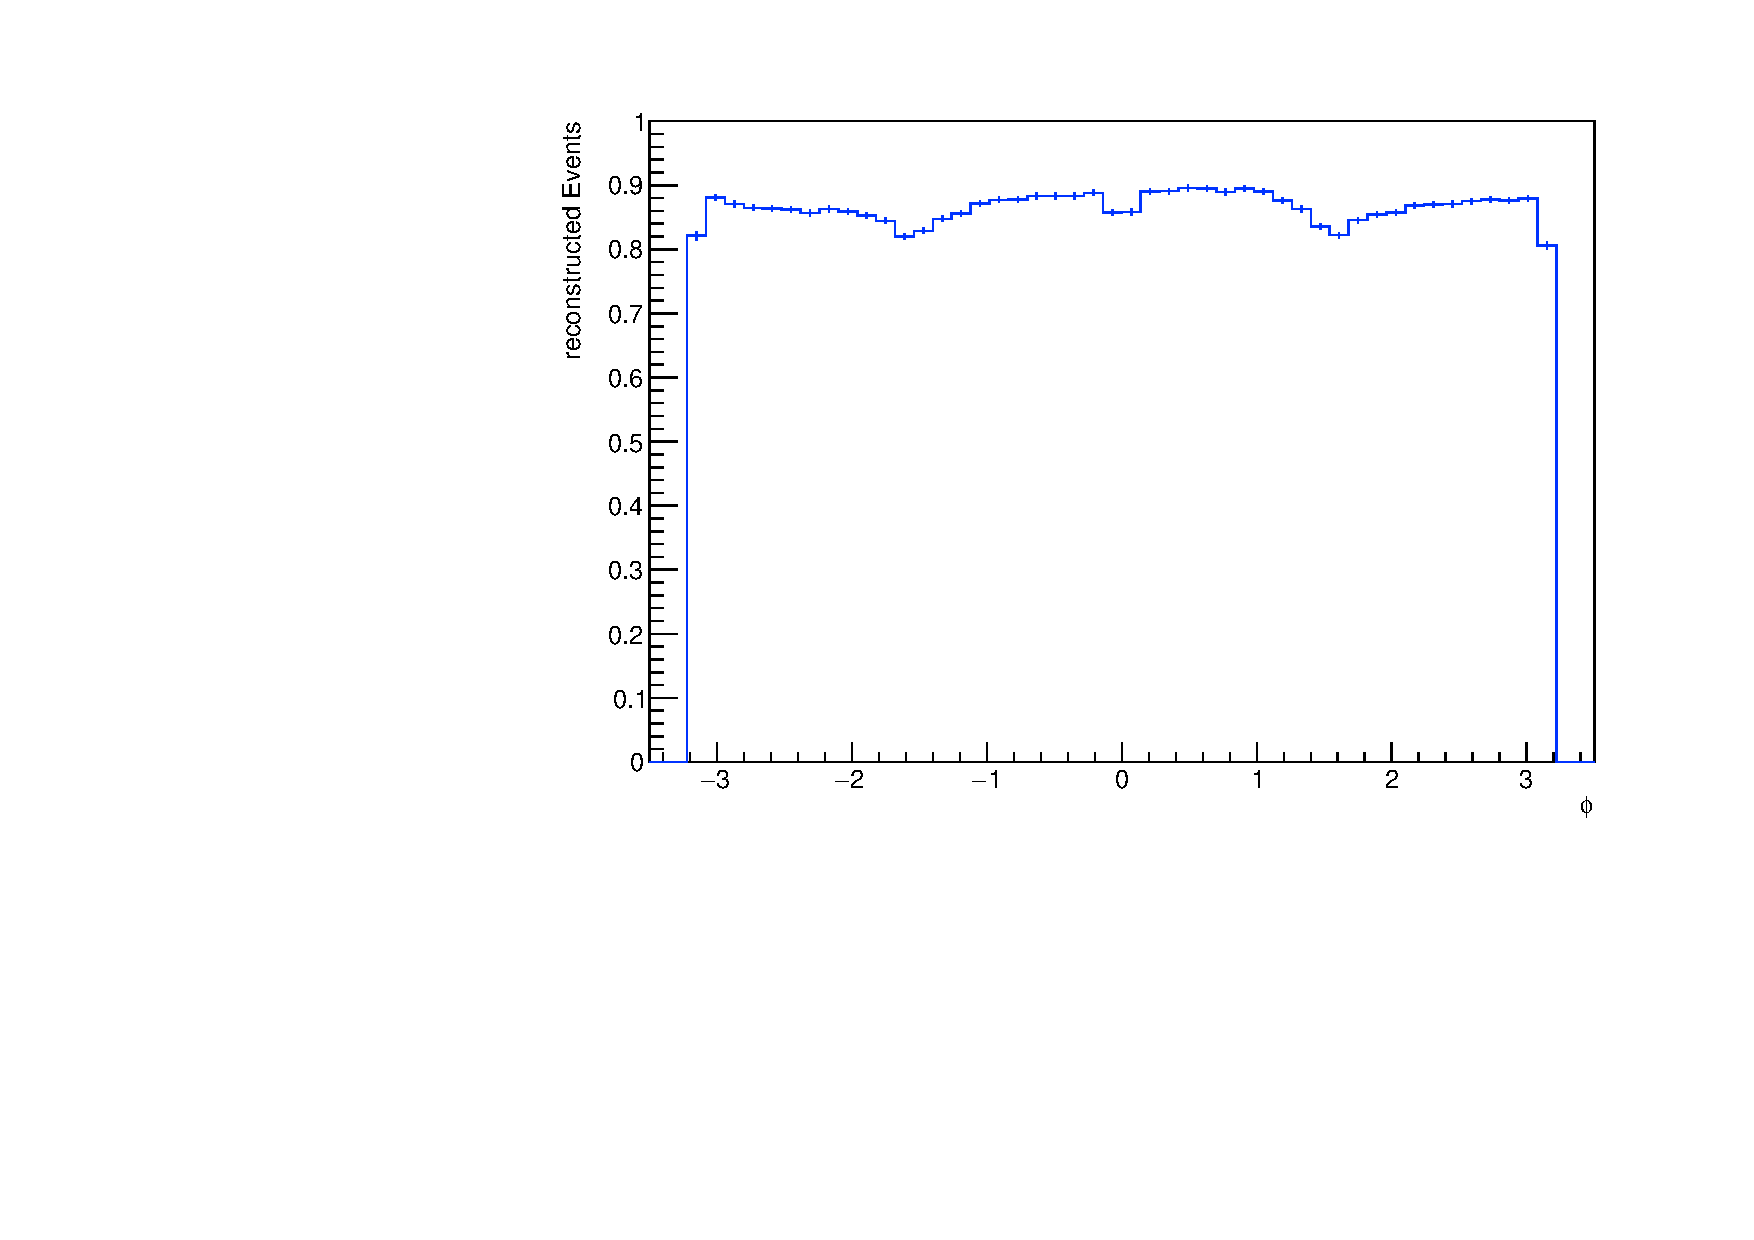
\includegraphics[width=0.9\textwidth]{up_pdf/single/neg/h_phi_reco_Pi_neg.pdf}
\end{subfigure}
\begin{subfigure}{0.45\textwidth}
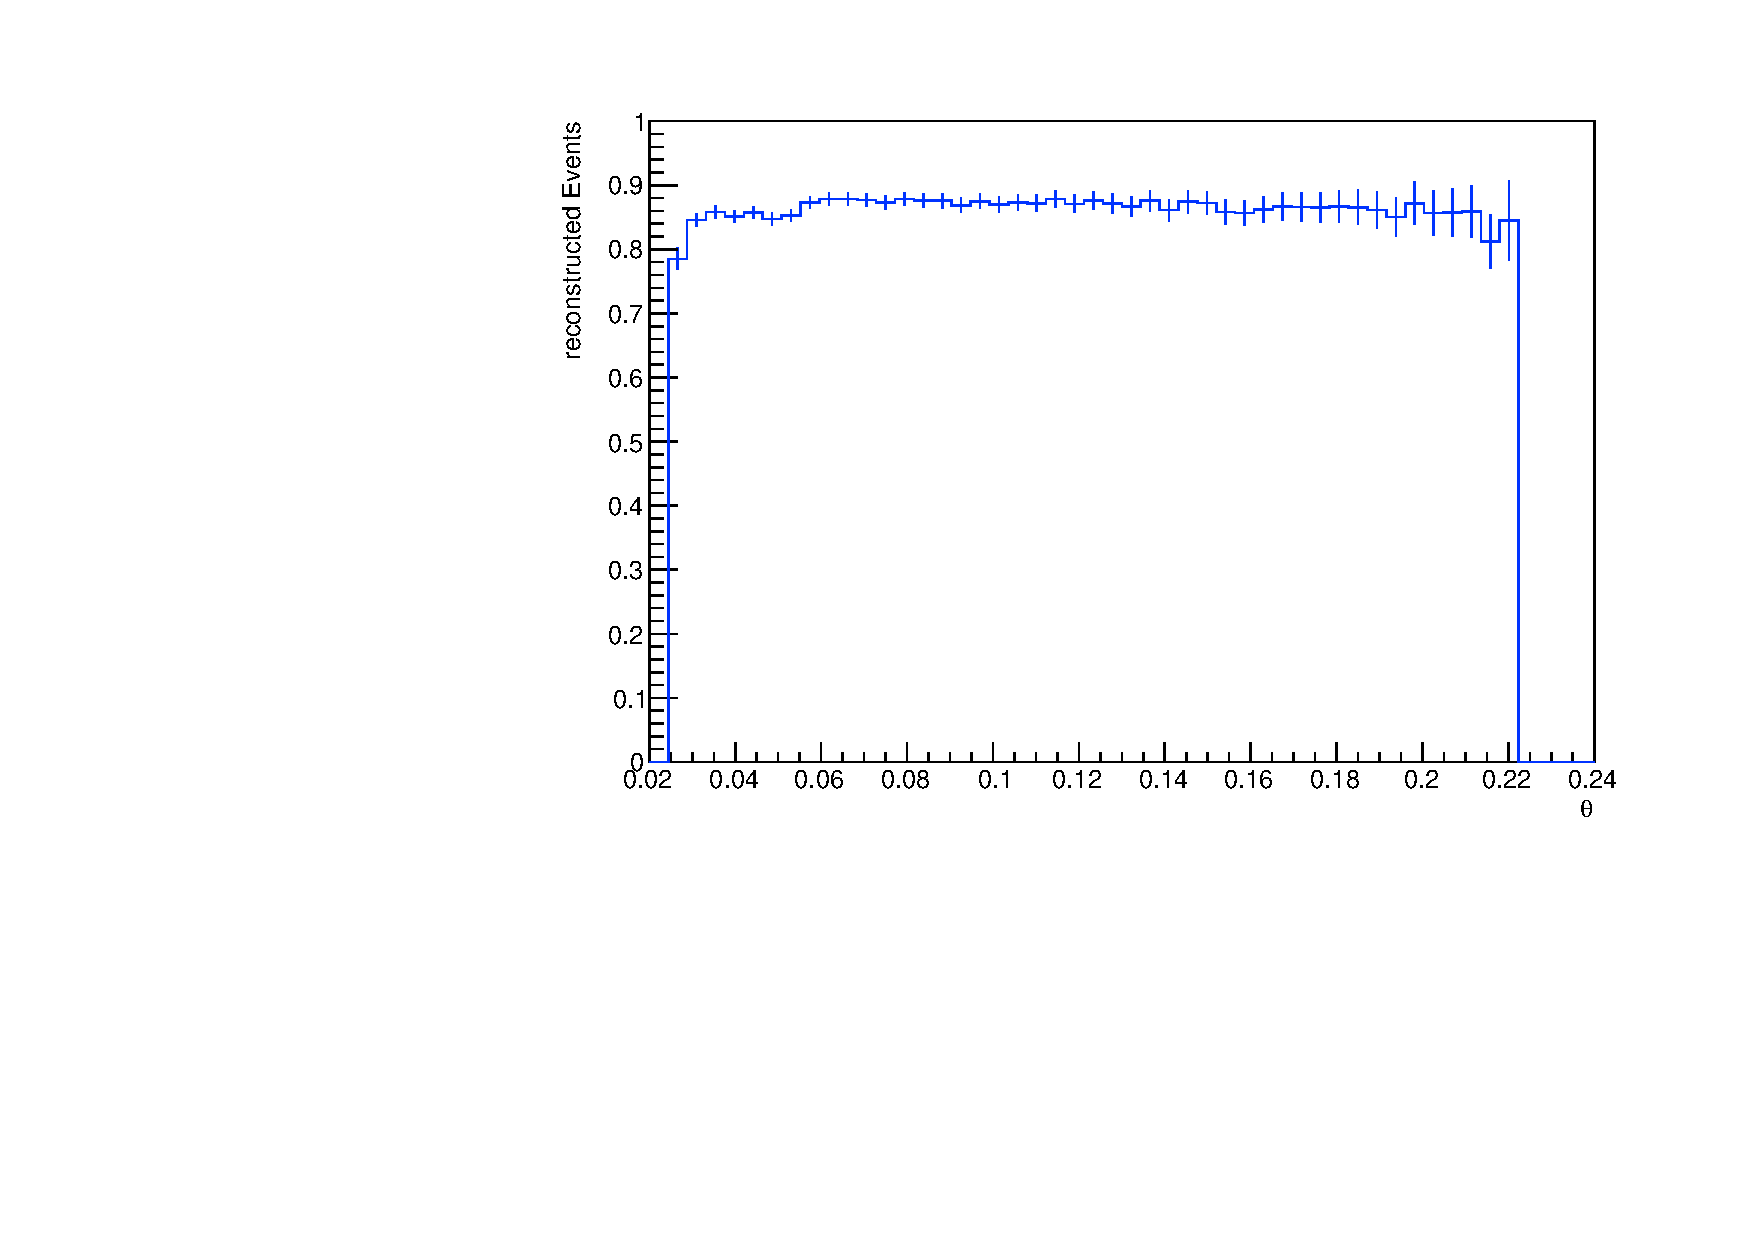
\includegraphics[width=0.9\textwidth]{up_pdf/single/neg/h_theta_reco_Pi_neg.pdf}
\end{subfigure}
\begin{subfigure}{0.45\textwidth}
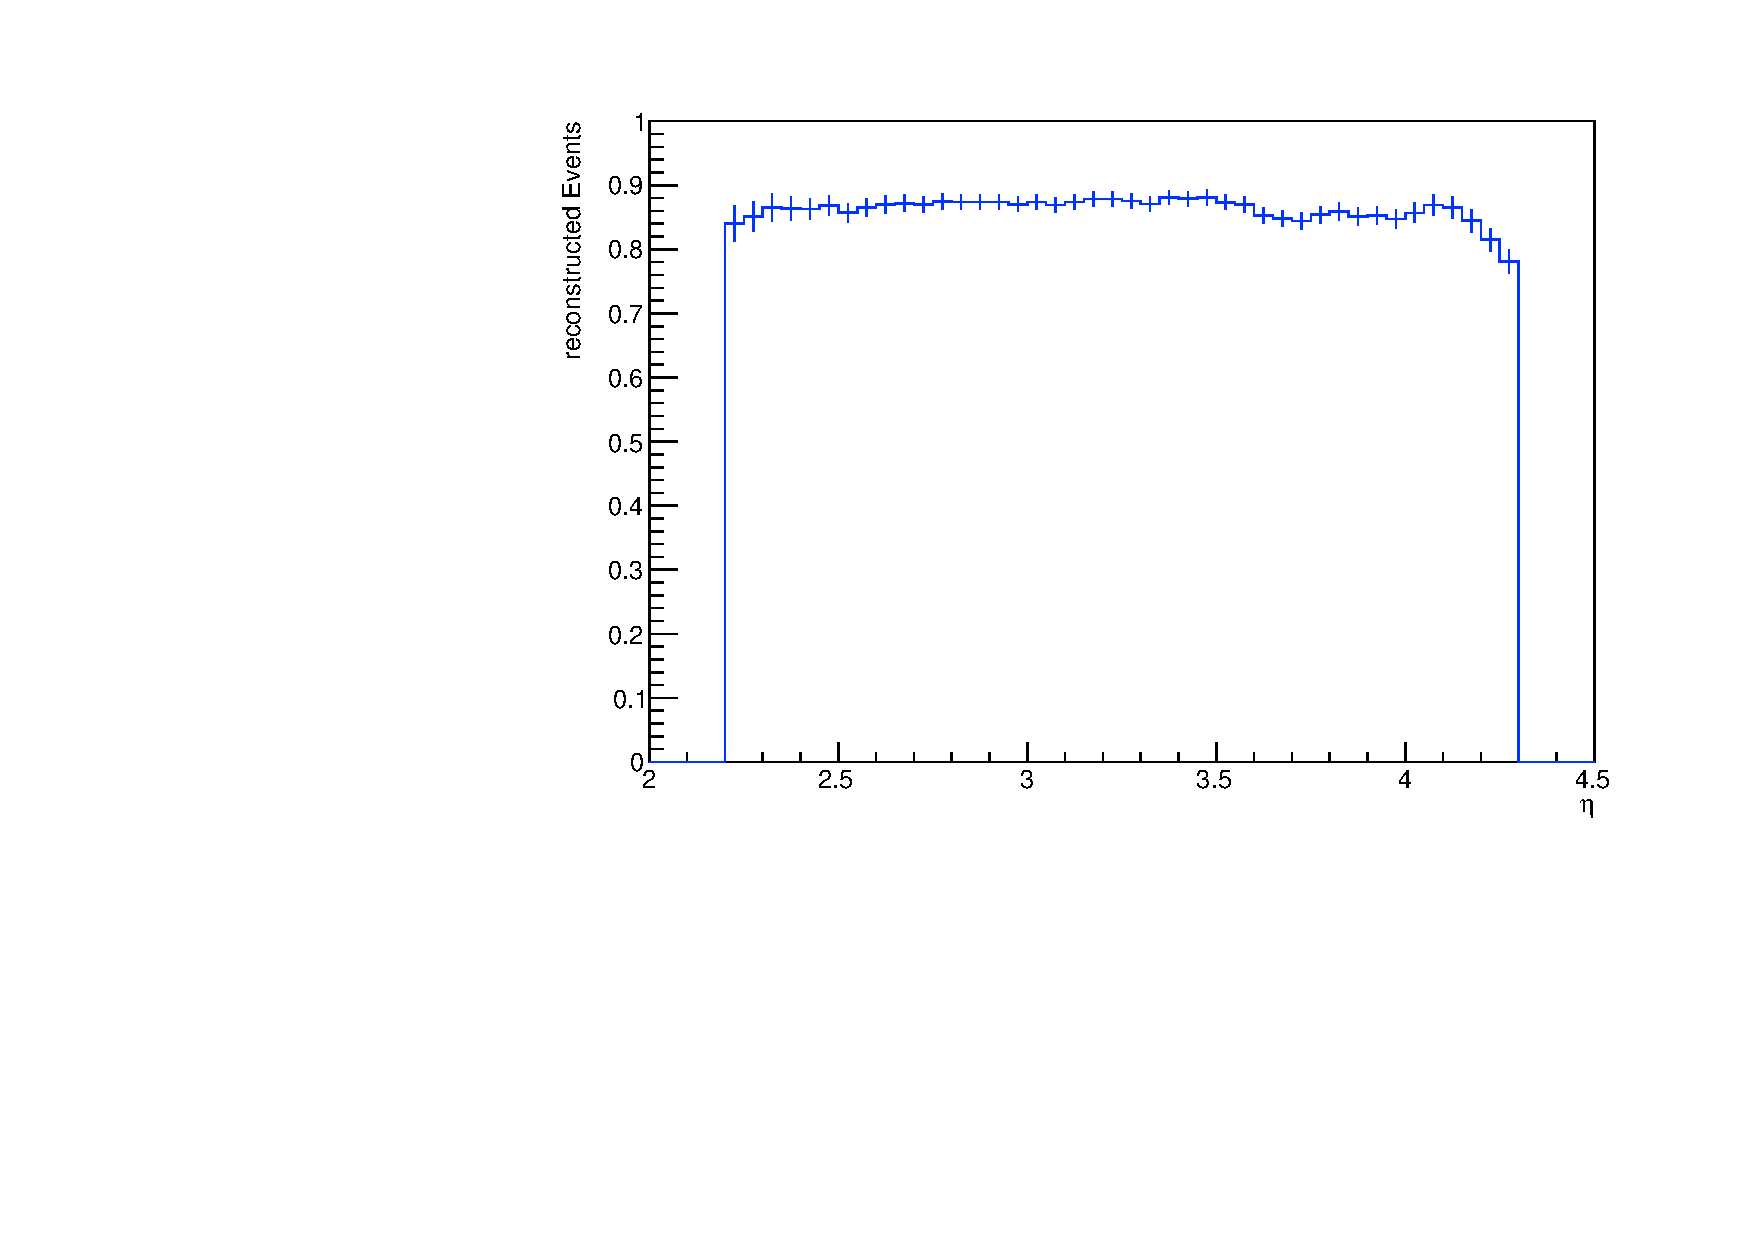
\includegraphics[width=0.9\textwidth]{up_pdf/single/neg/h_eta_reco_Pi_neg.pdf}
\end{subfigure}
\end{figure}
\end{frame}
\begin{frame}{$K$-efficiency}
\begin{figure}
\begin{subfigure}{0.45\textwidth}
\includegraphics[width=0.9\textwidth]{up_pdf/single/neg/h_pt_reco_K_neg.pdf}
\end{subfigure}
\begin{subfigure}{0.45\textwidth}
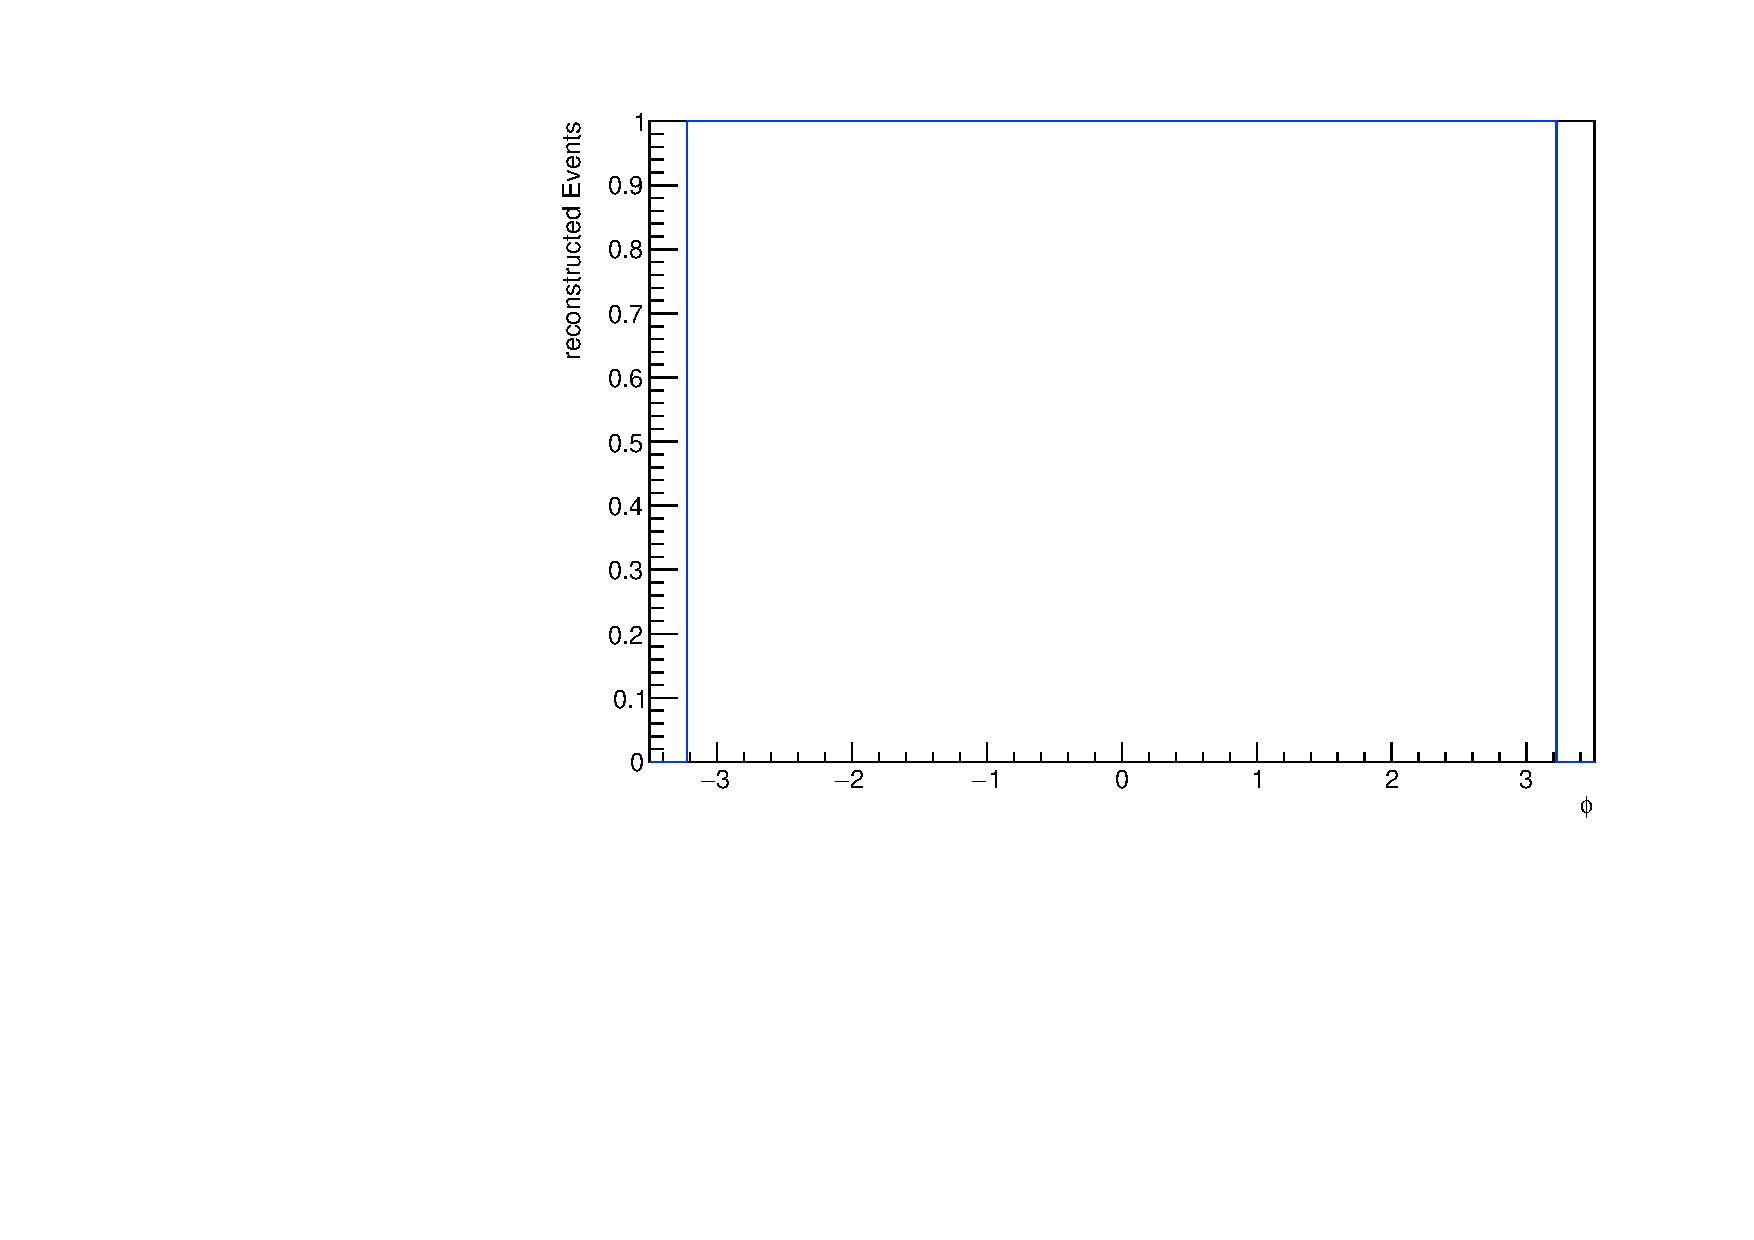
\includegraphics[width=0.9\textwidth]{up_pdf/single/neg/h_phi_reco_K_neg.pdf}
\end{subfigure}
\begin{subfigure}{0.45\textwidth}
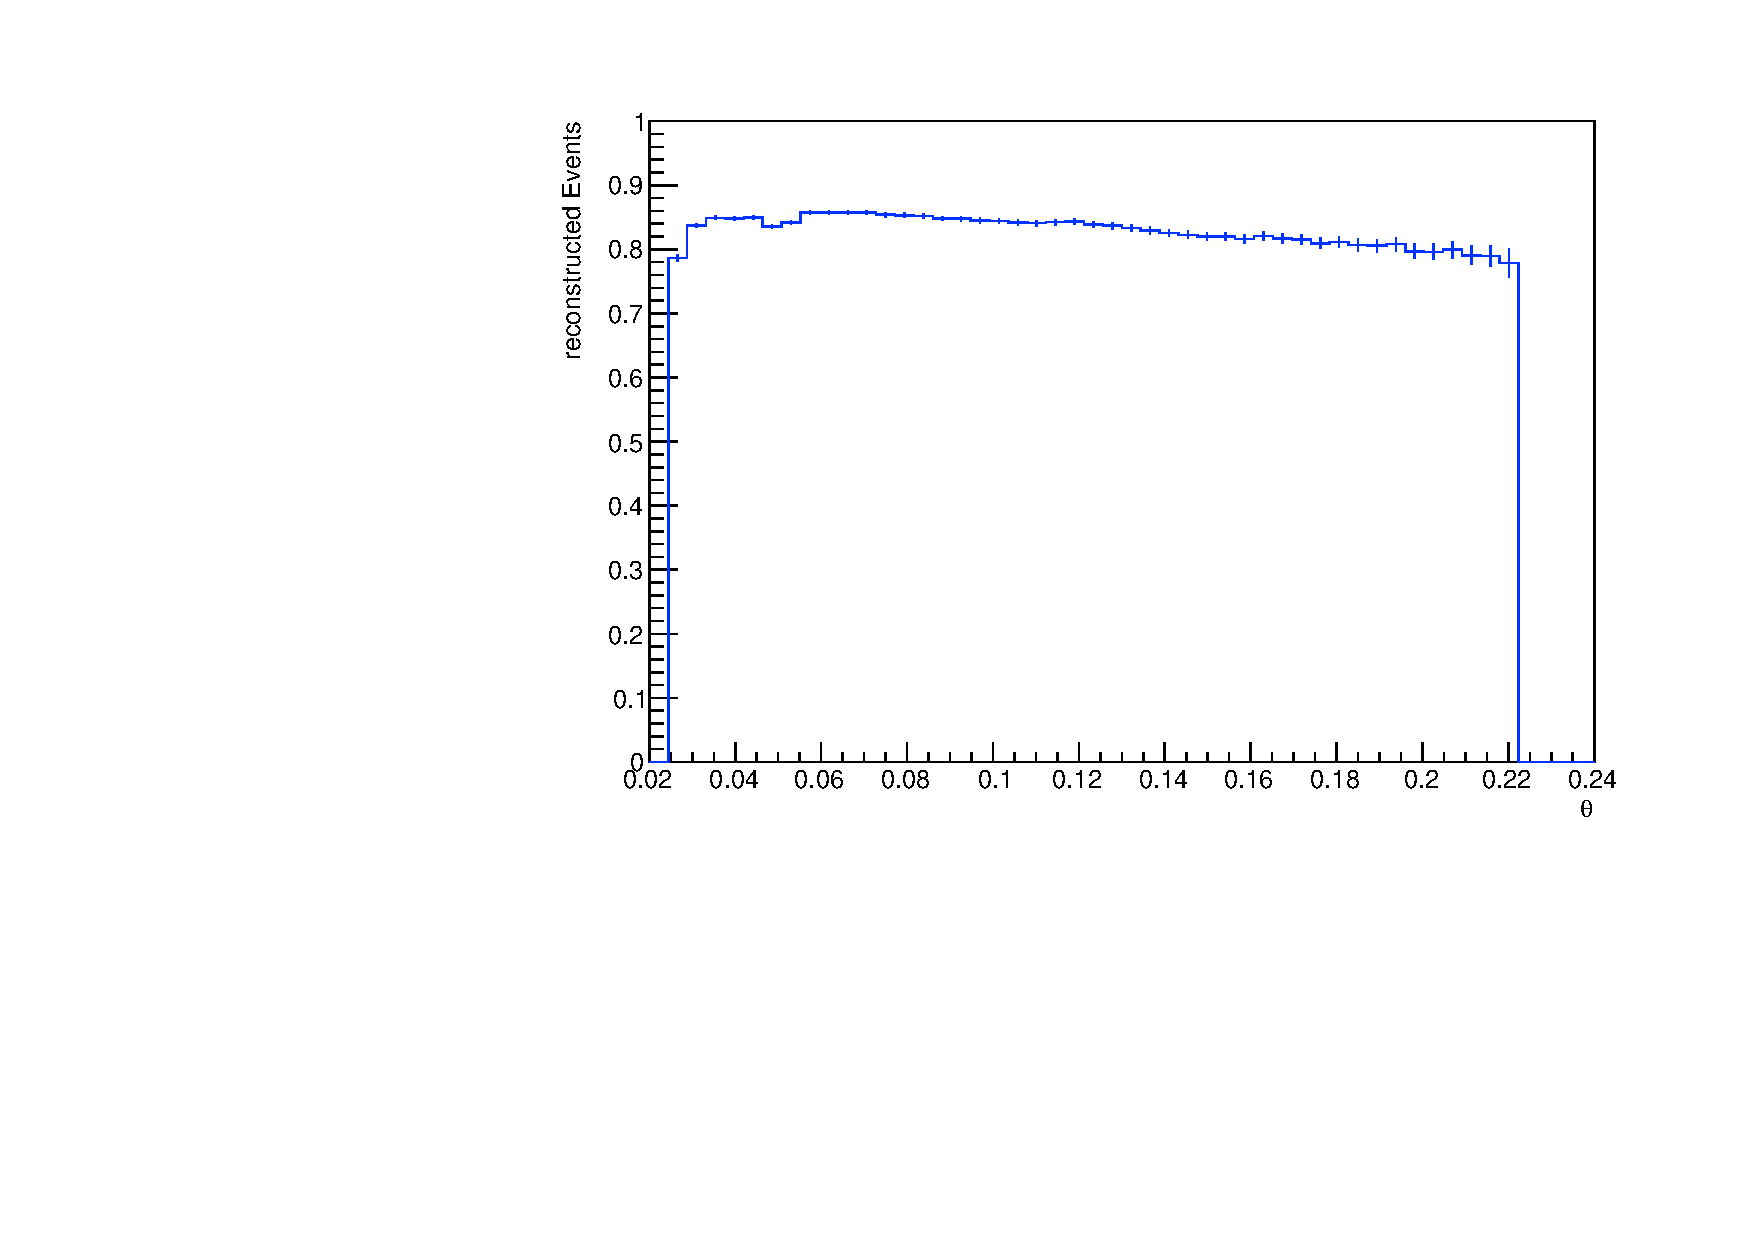
\includegraphics[width=0.9\textwidth]{up_pdf/single/neg/h_theta_reco_K_neg.pdf}
\end{subfigure}
\begin{subfigure}{0.45\textwidth}
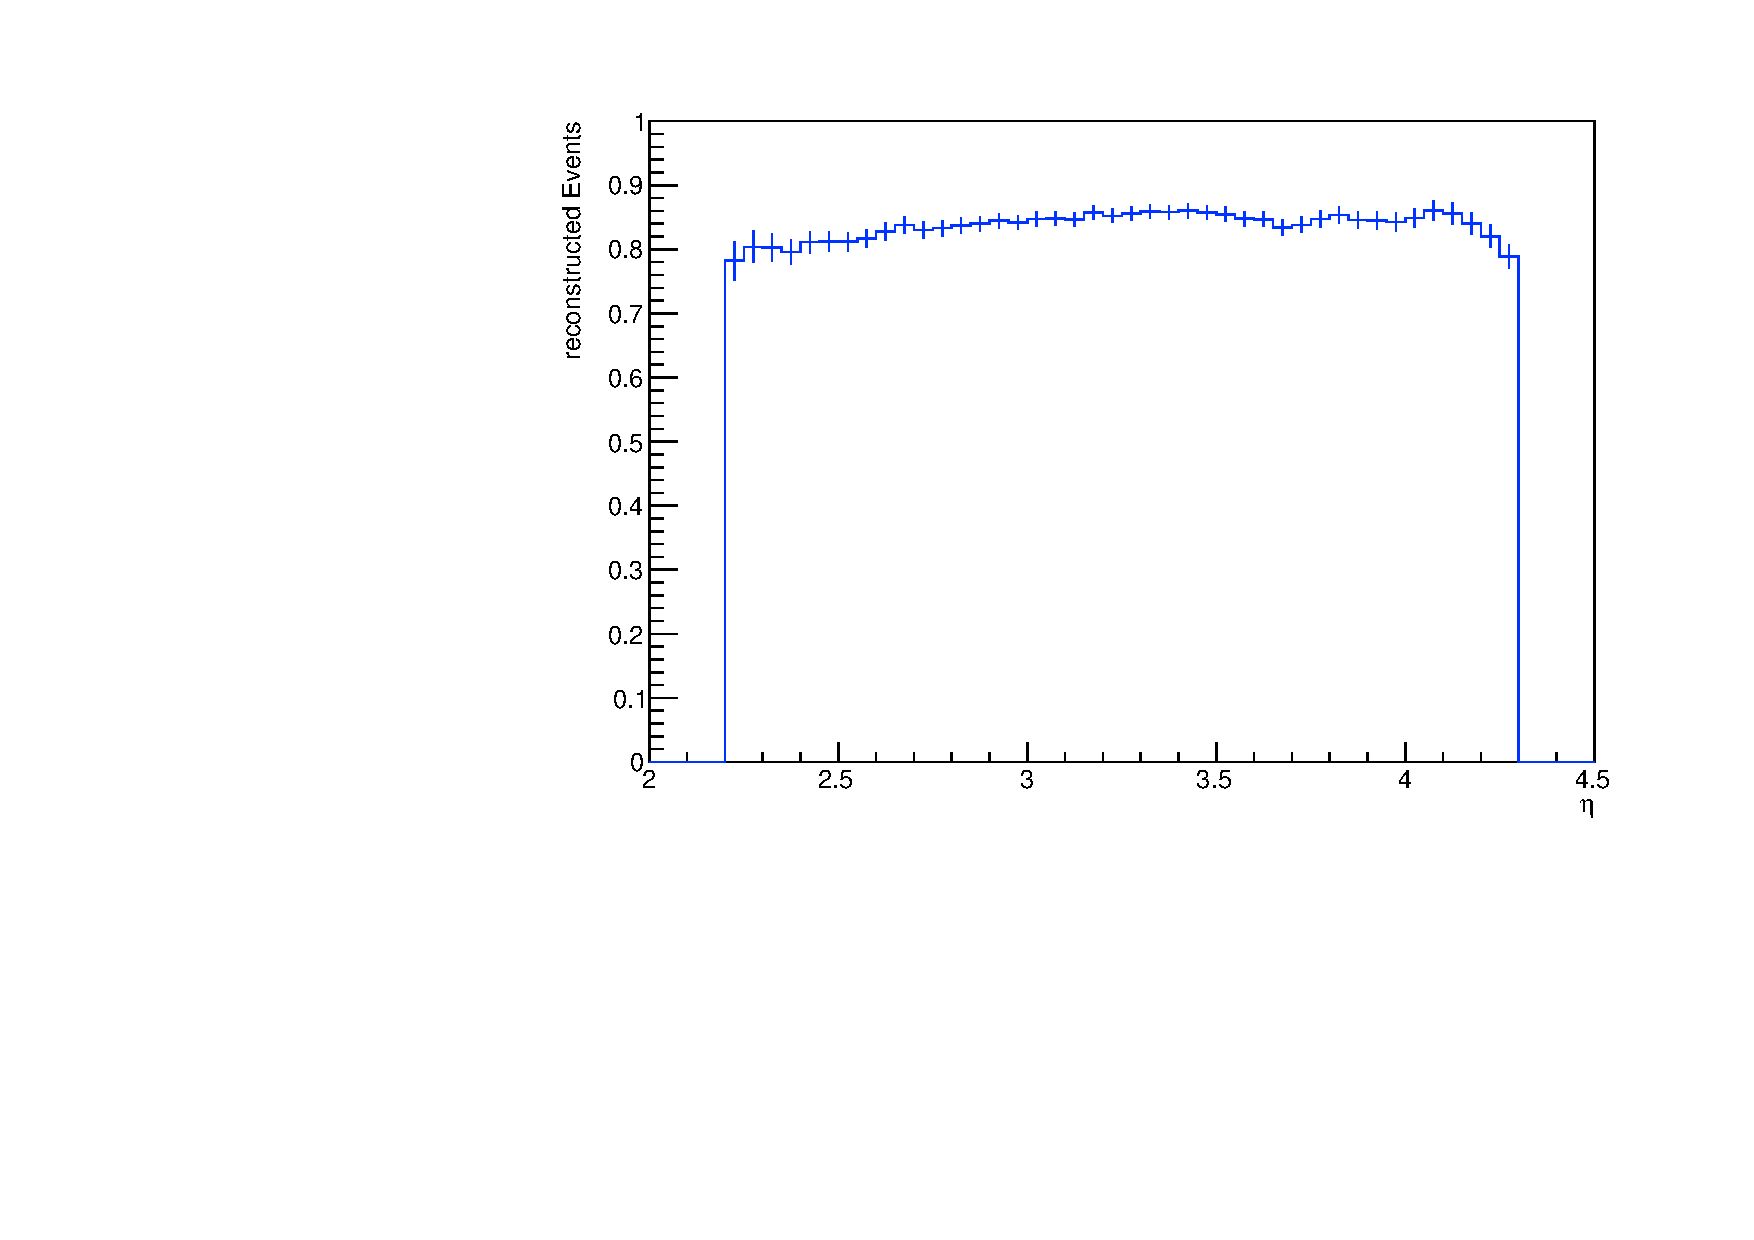
\includegraphics[width=0.9\textwidth]{up_pdf/single/neg/h_eta_reco_K_neg.pdf}
\end{subfigure}
\end{figure}
\end{frame}
\begin{frame}{soft $\pi$-efficiency}
\begin{figure}
\begin{subfigure}{0.45\textwidth}
\includegraphics[width=0.9\textwidth]{up_pdf/single/neg/h_pt_reco_SPi_neg.pdf}
\end{subfigure}
\begin{subfigure}{0.45\textwidth}
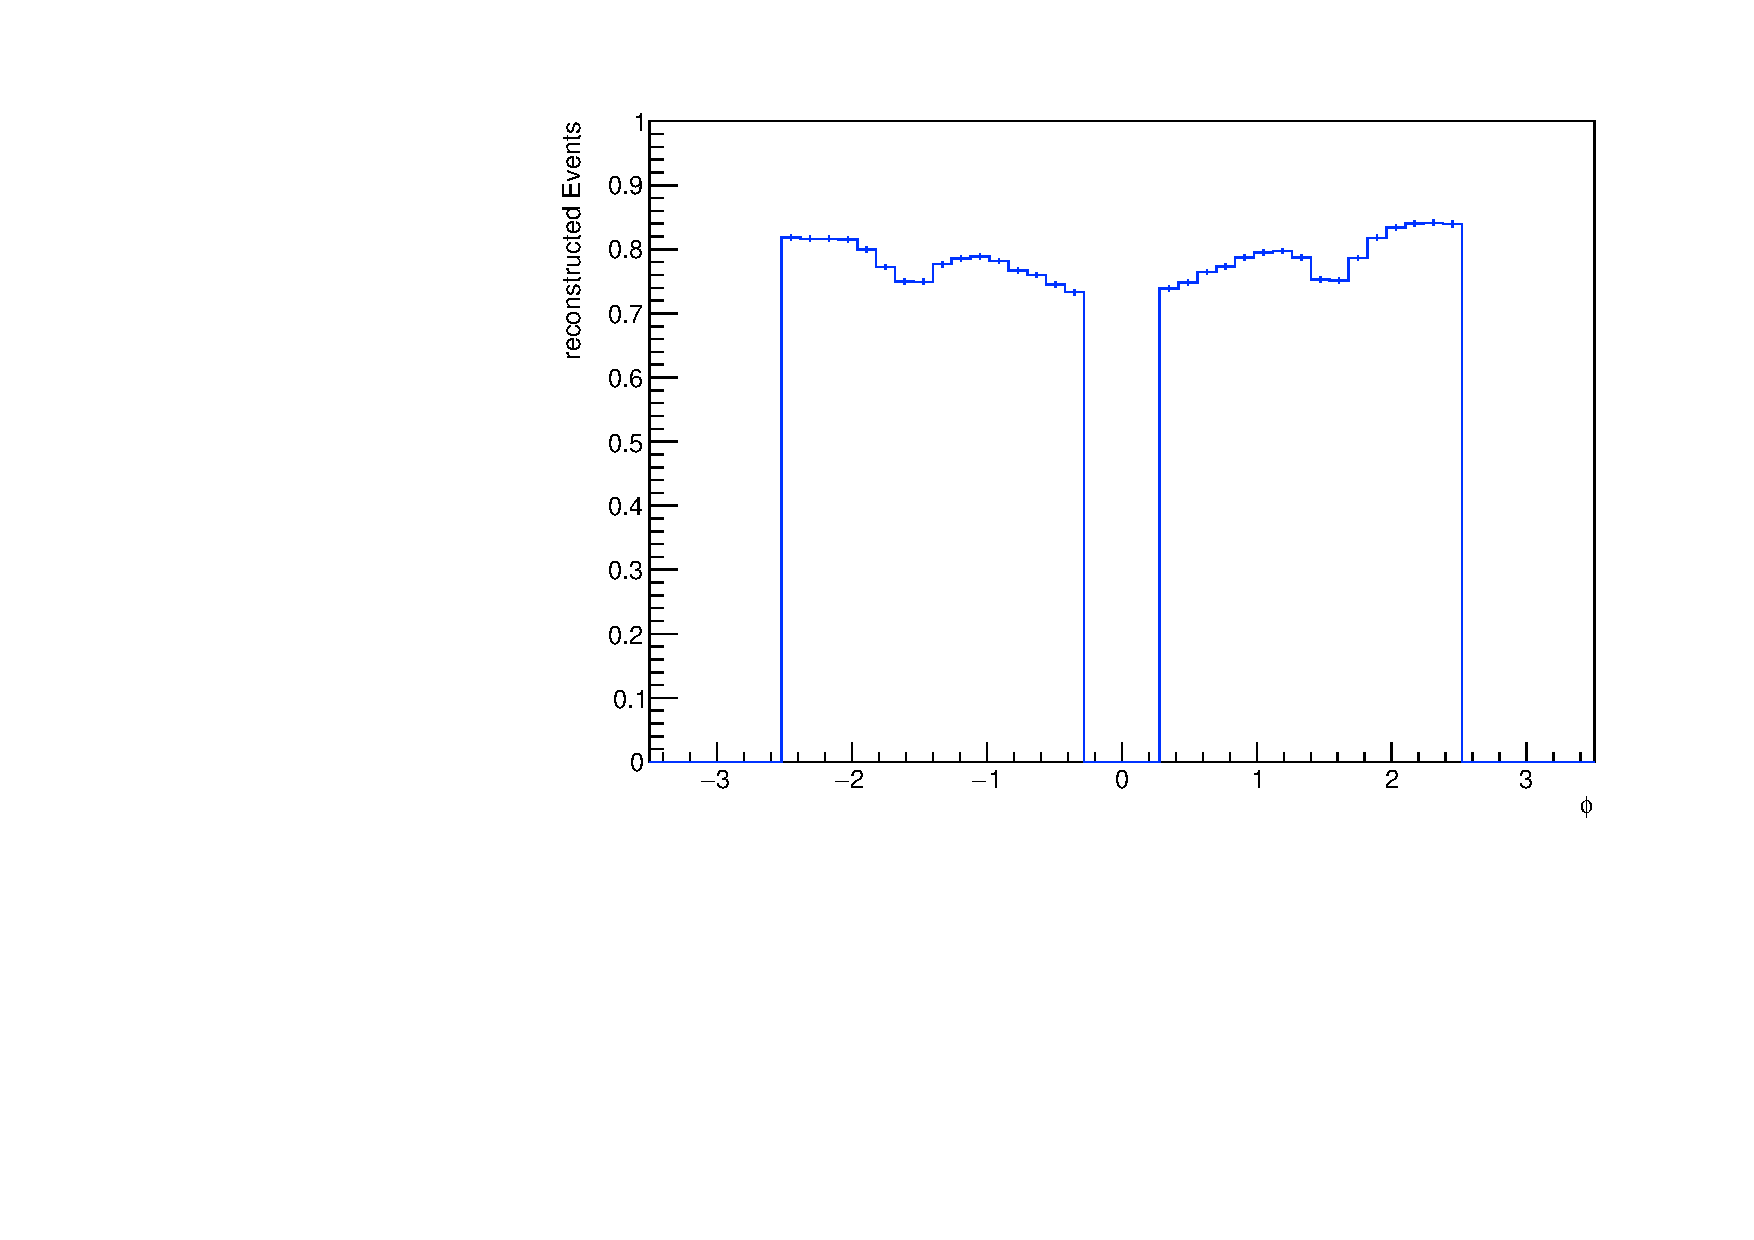
\includegraphics[width=0.9\textwidth]{up_pdf/single/neg/h_phi_reco_SPi_neg.pdf}
\end{subfigure}
\begin{subfigure}{0.45\textwidth}
\includegraphics[width=0.9\textwidth]{up_pdf/single/neg/h_theta_reco_SPi_neg.pdf}
\end{subfigure}
\begin{subfigure}{0.45\textwidth}
\includegraphics[width=0.9\textwidth]{up_pdf/single/neg/h_eta_reco_SPi_neg.pdf}
\end{subfigure}
\end{figure}
\end{frame}
\begin{frame}{$D^0$-efficiency}
\begin{figure}
\begin{subfigure}{0.45\textwidth}
\includegraphics[width=0.9\textwidth]{up_pdf/single/neg/h_pt_reco_D0_neg.pdf}
\end{subfigure}
\begin{subfigure}{0.45\textwidth}
\includegraphics[width=0.9\textwidth]{up_pdf/single/neg/h_phi_reco_D0_neg.pdf}
\end{subfigure}
\begin{subfigure}{0.45\textwidth}
\includegraphics[width=0.9\textwidth]{up_pdf/single/neg/h_theta_reco_D0_neg.pdf}
\end{subfigure}
\begin{subfigure}{0.45\textwidth}
\includegraphics[width=0.9\textwidth]{up_pdf/single/neg/h_eta_reco_D0_neg.pdf}
\end{subfigure}
\end{figure}
\end{frame}
\begin{frame}{$D^*$-efficiency}
\begin{figure}
\begin{subfigure}{0.45\textwidth}
\includegraphics[width=0.9\textwidth]{up_pdf/single/neg/h_pt_reco_Dst_neg.pdf}
\end{subfigure}
\begin{subfigure}{0.45\textwidth}
\includegraphics[width=0.9\textwidth]{up_pdf/single/neg/h_phi_reco_Dst_neg.pdf}
\end{subfigure}
\begin{subfigure}{0.45\textwidth}
\includegraphics[width=0.9\textwidth]{up_pdf/single/neg/h_theta_reco_Dst_neg.pdf}
\end{subfigure}
\begin{subfigure}{0.45\textwidth}
\includegraphics[width=0.9\textwidth]{up_pdf/single/neg/h_eta_reco_Dst_neg.pdf}
\end{subfigure}
\end{figure}
\end{frame}
\begin{frame}{Deviation}
\begin{table}
	\caption{The deviation $\frac{\epsilon_+ - \epsilon_-}{\epsilon_+ + \epsilon_-}/10^{-3}$}
	\resizebox{\textwidth}{!}{
	\begin{tabular}{cS[table-format=1.1]@{${}\pm{}$}S[table-format=1.1]S[table-format=1.1]@{${}\pm{}$}S[table-format=1.1]S[table-format=1.1]@{${}\pm{}$}S[table-format=1.1]S[table-format=1.1]@{${}\pm{}$}S[table-format=1.1]S[table-format=1.1]@{${}\pm{}$}S[table-format=1.1]}
		\toprule
		{Polarity} & \multicolumn{2}{c}{$\pi $} & \multicolumn{2}{c}{$ K $} & \multicolumn{2}{c}{$ soft \pi $} & \multicolumn{2}{c}{$ D^0 $} & \multicolumn{2}{c}{$ D^* $} \\
		\midrule
		$UP$ & 0.1 & 0.2 & 4.5 & 0.2 & -3.7 & 0.2 & -4.5 & 0.2 & -8.1 & 0.4 \\
		$DOWN$ & 0.2 & 0.2 & 4.7 & 0.2 & 4.2 & 0.2 & -4.5 & 0.2 & -0.3 & 0.4\\
		\bottomrule
	\end{tabular}}
	\caption{The deviation $\frac{N_+ - N_-}{N_+ + N_-}/10^{-3}$}
	\resizebox{\textwidth}{!}{
	\begin{tabular}{cS[table-format=1.1]@{${}\pm{}$}S[table-format=1.1]S[table-format=1.1]@{${}\pm{}$}S[table-format=1.1]S[table-format=1.1]@{${}\pm{}$}S[table-format=1.1]S[table-format=1.1]@{${}\pm{}$}S[table-format=1.1]S[table-format=1.1]@{${}\pm{}$}S[table-format=1.1]}
		\toprule
		{Polarity} & \multicolumn{2}{c}{$\pi $} & \multicolumn{2}{c}{$ K $} & \multicolumn{2}{c}{$ soft \pi $} & \multicolumn{2}{c}{$ D^0 $} & \multicolumn{2}{c}{$ D^* $} \\
		\midrule
		$UP$ & -0.1 & 0.4 & 4.7 & 0.4 & -3.8 & 0.5 & -4.7 & 0.5 & -8.2 & 0.5 \\
		$DOWN$ & -0.3 & 0.4 & 5.2 & 0.4 & 3.7 & 0.5 & -5.0 & 0.5 & -0.8 & 0.5\\
		\bottomrule
	\end{tabular}}
\end{table}
\begin{itemize}
\item calculation via $N_\text{reco}$ doesn't work, $N_\text{tot,+/-}$ different $\rightarrow$ no normalization
\item interesting: $D_{soft\,\pi} \& D_{D^0}$ cancel partially in $DOWN$,\\
but add up in $UP$
\end{itemize}
\end{frame}
\begin{frame}{Comparison of different charges with $UP$ polarity - $D^*$}
\begin{figure}
\begin{subfigure}{0.45\textwidth}
\includegraphics[width=0.9\textwidth]{up_pdf/combined/h_pt_reco_Dst.pdf}
\end{subfigure}
\begin{subfigure}{0.45\textwidth}
\includegraphics[width=0.9\textwidth]{up_pdf/combined/h_phi_reco_Dst.pdf}
\end{subfigure}
\begin{subfigure}{0.45\textwidth}
\includegraphics[width=0.9\textwidth]{up_pdf/combined/h_theta_reco_Dst.pdf}
\end{subfigure}
\begin{subfigure}{0.45\textwidth}
\includegraphics[width=0.9\textwidth]{up_pdf/combined/h_eta_reco_Dst.pdf}
\end{subfigure}
\end{figure}
\end{frame}
\begin{frame}{Comparison of different charges with $DOWN$ polarity - $D^*$}
\begin{figure}
\begin{subfigure}{0.45\textwidth}
\includegraphics[width=0.9\textwidth]{down_pdf/combined/h_pt_reco_Dst.pdf}
\end{subfigure}
\begin{subfigure}{0.45\textwidth}
\includegraphics[width=0.9\textwidth]{down_pdf/combined/h_phi_reco_Dst.pdf}
\end{subfigure}
\begin{subfigure}{0.45\textwidth}
\includegraphics[width=0.9\textwidth]{down_pdf/combined/h_theta_reco_Dst.pdf}
\end{subfigure}
\begin{subfigure}{0.45\textwidth}
\includegraphics[width=0.9\textwidth]{down_pdf/combined/h_eta_reco_Dst.pdf}
\end{subfigure}
\end{figure}
\end{frame}
\begin{frame}{Comparison - $D^* p_\text{T}$}
\centering
\includegraphics[width=0.48\textwidth]{up_pdf/combined/h_pt_reco_Dst.pdf}
\includegraphics[width=0.48\textwidth]{down_pdf/combined/h_pt_reco_Dst.pdf}
\end{frame}
\begin{frame}{Comparison - $D^* \phi$}
\centering
\includegraphics[width=0.48\textwidth]{up_pdf/combined/h_phi_reco_Dst.pdf}
\includegraphics[width=0.48\textwidth]{down_pdf/combined/h_phi_reco_Dst.pdf}
\end{frame}
\begin{frame}{Comparison - $D^* \theta$}
\centering
\includegraphics[width=0.48\textwidth]{up_pdf/combined/h_theta_reco_Dst.pdf}
\includegraphics[width=0.48\textwidth]{down_pdf/combined/h_theta_reco_Dst.pdf}
\end{frame}
\begin{frame}{Comparison - $D^* \eta$}
\centering
\includegraphics[width=0.48\textwidth]{up_pdf/combined/h_eta_reco_Dst.pdf}
\includegraphics[width=0.48\textwidth]{down_pdf/combined/h_eta_reco_Dst.pdf}
\end{frame}
\begin{frame}{$D^*$ deviation dependencies - $UP$ polarity}
\begin{figure}
\begin{subfigure}{0.45\textwidth}
\includegraphics[width=0.9\textwidth]{up_pdf/deviation/h_pt_reco_Dst_pos.pdf}
\end{subfigure}
\begin{subfigure}{0.45\textwidth}
\includegraphics[width=0.9\textwidth]{up_pdf/deviation/h_phi_reco_Dst_pos.pdf}
\end{subfigure}
\begin{subfigure}{0.45\textwidth}
\includegraphics[width=0.9\textwidth]{up_pdf/deviation/h_theta_reco_Dst_pos.pdf}
\end{subfigure}
\begin{subfigure}{0.45\textwidth}
\includegraphics[width=0.9\textwidth]{up_pdf/deviation/h_eta_reco_Dst_pos.pdf}
\end{subfigure}
\end{figure}
\end{frame}
\begin{frame}{$D^*$ deviation dependencies - $DOWN$ polarity}
\begin{figure}
\begin{subfigure}{0.45\textwidth}
\includegraphics[width=0.9\textwidth]{down_pdf/deviation/h_pt_reco_Dst_pos.pdf}
\end{subfigure}
\begin{subfigure}{0.45\textwidth}
\includegraphics[width=0.9\textwidth]{down_pdf/deviation/h_phi_reco_Dst_pos.pdf}
\end{subfigure}
\begin{subfigure}{0.45\textwidth}
\includegraphics[width=0.9\textwidth]{down_pdf/deviation/h_theta_reco_Dst_pos.pdf}
\end{subfigure}
\begin{subfigure}{0.45\textwidth}
\includegraphics[width=0.9\textwidth]{down_pdf/deviation/h_eta_reco_Dst_pos.pdf}
\end{subfigure}
\end{figure}
\end{frame}
\begin{frame}{$D^*$ deviation - $\phi$}
\centering
\includegraphics[width=0.48\textwidth]{up_pdf/deviation/h_phi_reco_Dst_pos.pdf}
\includegraphics[width=0.48\textwidth]{down_pdf/deviation/h_phi_reco_Dst_pos.pdf}
\begin{itemize}
\item left $UP$, right $DOWN$
\item clear dependency in $\phi$, inverted $UP\leftrightarrow DOWN$
\item doesn't seem to have dependency on other topological variables\\
$\rightarrow$ form of the detector is biggest source of induced CPV
\end{itemize}
\end{frame}
\begin{frame}{$D^*$ deviation UP+DOWN}
\begin{figure}
\begin{subfigure}{0.45\textwidth}
\includegraphics[width=0.9\textwidth]{up_plus_down_pdf/pT_4.pdf}
\end{subfigure}
\begin{subfigure}{0.45\textwidth}
\includegraphics[width=0.9\textwidth]{up_plus_down_pdf/phi_4.pdf}
\end{subfigure}
\begin{subfigure}{0.45\textwidth}
\includegraphics[width=0.9\textwidth]{up_plus_down_pdf/theta_4.pdf}
\end{subfigure}
\begin{subfigure}{0.45\textwidth}
\includegraphics[width=0.9\textwidth]{up_plus_down_pdf/eta_4.pdf}
\end{subfigure}
\end{figure}
\end{frame}
\end{document}


%♥